\documentclass[mres, copyrightpage]{mqthesis}
%----------------------------------------------------------
% OPTIONS
% Options you can use in the documentclass above:
%
% phd/mres/hons = set the degree text [default=phd]
% copyrightpage d= print a copyright page on the back 
%                 of the title page [default=false]
% examinerscopy = print "Examiner's Copy" of title page and 
%                 change linespacing to 1.5 [default=false]
% greychapternumbers = print large chapter numbers in grey
%                 instead of MQ corporate "sand"
%---------------------------------------------------------- 

% this shows what labels you are using for cross references
% \usepackage{showkeys} 

%---------------------------------------------------------- 
% STRUCTURE
% this document is a skeleton which pulls in the meat of the thesis
% from other files. Comment out and add lines as appropriate.
%---------------------------------------------------------- 

\usepackage{pdflscape}
\begin{document}

%---------------------------------------------------------- 
% FRONT
% Acknowledgements, titlepage, abstract, list of publications
%---------------------------------------------------------- 
\frontmatter

\title{Logic-Based Benders Decomposition applied to the Setup Assembly Line Balancing and Scheduling Problem}
\author{Kenneth Young}
\department{School of Mathematics and Statistics}  % put your department here

\titlepage

\chapter{Acknowledgements}
\label{chap:ack}

This thesis is a result of almost two years 
of research undertaken at the University of Melbourne.
As my first major step into the world of academic
research, I can say that this project has been 
extremely challenging, whilst also tremendously rewarding.
During the final semester of the research project, my life
was filled with modelling, coding, debugging,
more debugging and writing.
Each of which was thoroughly enjoyable.

All the wonderful people which I was surrounded
by deserve a non-trivial share of the credit.
Their help and encouragement throughout the project has been invaluable,
and for that I am grateful.

First and foremost, I must thank the one who deserves it the most,
Alysson Costa, my supervisor.
Without his guidance, this project may have taken numerous wrong turns
along the way.
Alysson has previously studied both the problem I tackled
and the method I have used, and so his familiarity with the
areas provided a much needed level of understanding in the early days of the project.
I really appreciate the theoretical contributions that Alysson has
made, but possibly more importantly,
I truly appreciate his kindness.
He has an uncanny ability to find the humour in life
and seems to always have an extra smile to offer when one is needed.
It has been a pleasure to work with the most enthusiastic Operations
Researcher I've met.

My friends, both old and new, have filled these days 
of my life with jokes, pranks and joy; and I cannot thank them
enough for it.
I wish to thank Ai, Anupama, Ali, Ria, Lotte, Mark, Mim, 
Shian, John, Curtis, Heather, Scott, Lachlan, 
Georgia, Ben, Constance and Vincent.
In particular, Ria's help and friendship over the whole course
of my Masters needs a special mention.
Working together on the group projects during our course
has been nothing but a pleasure.
Her drive to become the very best she can --- at anything she puts her mind to ---
has been contagious.
Even in this thesis, her contributions to extending the
formulations of the CP sub-problems were pivotal in their successful performance.

I wish to express my gratitude to my sister, Margaret.
Miraculously, all the house work that I was unable to
assist with this semester disappeared without
request or mention: for this I am thankful.
She provided an immense amount of help by taking the time
out of her life to
assist me in the proof reading process.
I thank Margaret for ensuring the reader does not need
to endure a complete butchering of the English language.

The fellow members of my research group have also provided
wonderful feedback during the course of this project.
Without fail, they have been able to find new fruitful directions to take the project,
whilst also steering me away from the directions not filled with quite so much fruit.
I wish to thank Landir, Allen, Cheng, Gala, Ashwani, Simran, Pamela and Chathranee.

The entire experience has been terrific.

And I would like to disacknowledge my mortal enemy, Anupama Pilbrow.
% \chapter{List of Publications}

\begin{itemize}
\item[$\bullet$] insert author list \emph{insert paper title}.  (submitted to
	insert journal name)
\item[$\bullet$] insert author list \emph{insert paper title}.  
        insert journal name \textbf{insert volume number}, 
        insert article or page number (insert year)
\end{itemize}

\chapter{Abstract}

Balancing the workload of an assembly line
leads to a decision problem where the aim is to
assign a set of tasks to a sequence of work stations,
whilst optimising a measure of performance, \eg maximising the production
rate.
The SetUp Assembly Line Balancing and Scheduling Problem (\sua{})
is a recent variant on the classical Assembly Line Balancing Problem (\albp{}).
This new problem introduces sequence-dependent
setup times between any pair of consecutive tasks
processed within a work station's task sequence.
Considering these setup times leads an additional layer
of complexity as the problem now involves a set
of scheduling decisions for each station along the production line.

Benders decomposition naturally suggests itself as an appropriate
approach for the \sua{} as we can divide the problem's decisions
into two distinct sets.
We propose a general logic-based Benders decomposition framework which 
leads to the assignment portion being decided by a relaxed
master problem and a number of sub-problems which together
handle the scheduling portion.
Each sub-problem is highly combinatorial in nature and so
we consider state-of-the-art solving technology from
both Operations Research and Artificial Intelligence
to solve the scheduling problem efficiently.
% We provide a detailed experimental analysis into the superior 
% sub-problem formulation
A range of Benders cuts are devised 
and their practical effectiveness
is one of our primary contributions to the 
literature.

We test the best-known exact methods to solve
the \sua{} and use these models
as a benchmark against which to scrutinise our hybrid solution methodology.
In total, 396 instances of the problem were tested and our Benders
decomposition approach vastly outperformed the best models from the literature.
Due to this variant of the \albp{} being notably under-studied,
we conclude the paper by remarking on a range of possible future directions
which the research community could investigate.


\tableofcontents
% comment out these as required for your discipline
\listoffigures
\listoftables

%---------------------------------------------------------- 
% MAIN
% include chapters as neededlmodern
%---------------------------------------------------------- 
\mainmatter

% Introduction
%!TEX root = thesis-kdyoung.tex

% \begin{savequote}%[45mm]
% If people do not believe that mathematics is simple, it is only because they do not realize how complicated life is.
% \qauthor{John von Neumann}
% \end{savequote}
\begin{savequote}%[45mm]
---Everything should be made as simple as possible, but not simpler.
\qauthor{Albert Einstein}
\end{savequote}

\chapter{Introduction}
\label{chap:intro}
Assembly lines are flow-based production systems widely used by
the manufacturing industry.
Designing these systems to meet the requirements set
by the industry gives rise to the Assembly Line
Balancing Problem (\albp{}).
An assembly line problem consists of a sequence
of \emph{stations} and a set of \emph{tasks}.
Stations are fixed points along the assembly
line which are operated by either human personnel
or autonomous machinery.
A workpiece is launched down the line and 
a subset of the tasks are performed on it at each station.
Once all required tasks are finished, the completed product
exits the assembly line.
% The construction of a single product is completed
% once all tasks have performed on it 
% To completely construct a single product
% the all tasks are performed along the line.
The workload of tasks must be divided among the stations
to optimize some performance measure,
while also respecting physical restrictions.
A standard example of such a restriction would be a
precedence relation, which can require
one task to be completed before another can begin
processing on the product.
The line itself is a mechanism used to
transport the products between stations;
most commonly the line is a conveyor belt.

There are two common objectives when designing an assembly
line, which each lead a distinct problem.
The first is called the type-1 problem and is concerned with
the design of a new assembly where the production rate
of the product is predefined and the aim is to construct the line
with as few stations as possible, in-order to meet this demand.
The second problem, called type-2, considers the redesign of an existing
assembly line where the number of stations is fixed and the rate
of production is optimized.
The second case can arise when a manufacturing company alters their
production process or changes the products they offer.
Our thesis focuses on solving the type-2 problem.

The \emph{cycle time} of an assembly line defines the time each station
is given to perform its assigned tasks.
As such, finding the minimal possible cycle time 
is the primary aim when optimizing the production
rate of an assembly line.
Since all stations are connected by a single line,
the station with the largest workload will define the
overall cycle time of the line.
To achieve the minimal cycle time value,
we aim to balance the workload of the tasks
as evenly as possible among the stations.

The structure of the paper is as follows.
The remainder of Chapter \ref{chap:intro}
provides illustrative examples of the problem
and closes with some motivation.
In Chapter \ref{chap:theory} we detail a selection
of the relevant theory for our problem, spanning
the fields of Operations Research and Artificial Intelligence.
Chapter \ref{chap:mip} presents the mixed-integer
programs which were used to compare our
solution methodology against.
The construction of our logic-based Benders
decomposition is presented in Chapter \ref{chap:benders},
together with many possible modelling choices.
The results of our computational experiments are 
given in Chapter \ref{chap:exp}.
We conclude in Chapter \ref{chap:conc}
with some remarks on the performance of our
method and finally note a range of possible directions
for future research on this topic.

\section{Preliminaries and Examples}
\label{sec:intro:prelim}
The fundamental problem in this area is called the
Simple \albp{}, or \sab{}; we denote
the type-2 version by \sab{2}.
We now detail some straightforward examples
to illustrate how the workload
of an assembly line can be balanced.
In Example \ref{ex:intro:simple} we provide an instance
of the \sab{2} with a possible feasible solution and the optimal solution given
in Figures \ref{fig:intro:exSchedFeas} and \ref{fig:intro:exSchedOpt}
respectively. Note, that $t_i$ denotes the processing time of task $i$ and
$c$ denotes the cycle time of the assembly line.

\begin{example}\label{ex:intro:simple}
	Consider an instance of the problem with four tasks $T_1,\ldots,T_4$,
	and three stations $S_1,\ldots,S_3$,
	along the assembly line.
	The aim is to find an assignment of the tasks to the stations
	which minimizes the cycle time.
	This assignment must respect the precedence relations listed in Figure \ref{fig:intro:exPrec}, 
	\eg task $T_1$ must be completed before task $T_2$.
	The processing time of each task is included in Figure \ref{fig:intro:exPrec}
	next to each task.

	A feasible solution to this problem is given in Figure \ref{fig:intro:exSchedFeas},
	where the stations are spaced along the horizontal axis.
	Each station's workload begins at the horizontal axis and proceeds
	upward through time until all assigned tasks are completed.
	In this solution, the workload of $S_3$ is the largest
	and as such defines the cycle time as $t_3+t_4=2+9=11$.

	This feasible solution can be improved by moving task $T_3$ from station
	$S_3$ to $S_2$.
	For this assignment to remain feasible, $T_3$ must be processed
	after $T_2$, due to the precedence relations.
	This new assignment leads to the optimal solution listed in
	Figure \ref{fig:intro:exSchedOpt} with a cycle time of nine.	\qed
\end{example}

\begin{figure}[tpb]
	\centering
	\caption{Precedence graph}
	\vspace{2mm}
	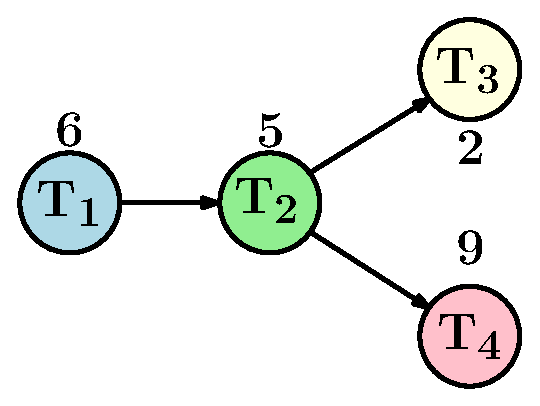
\includegraphics[width=0.45\textwidth]{images/precgraphSimple.eps}
	\label{fig:intro:exPrec}
\end{figure}

\begin{figure}[tpb]
	\centering
	\begin{minipage}{0.45\textwidth}
		\centering
		\caption{Feasible solution}
		\vspace{2mm}
		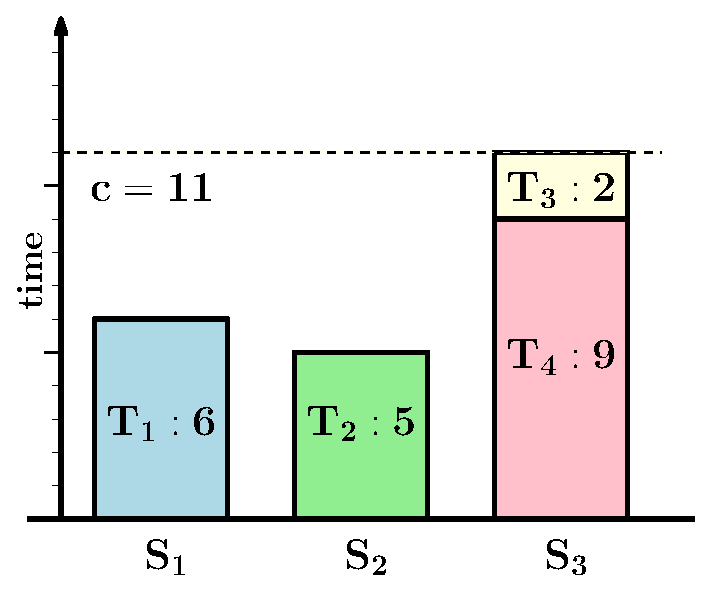
\includegraphics[width=\linewidth]{images/exSimpleFeas.eps}
		\label{fig:intro:exSchedFeas}
	\end{minipage}
	\hfill
	\begin{minipage}{0.45\textwidth}
		\centering
		\vfill
		\caption{Optimal solution}
		\vspace{2mm}
		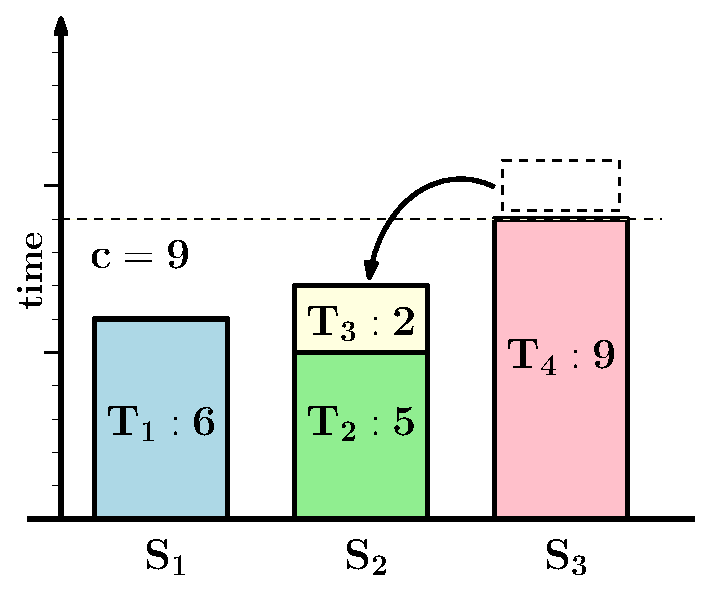
\includegraphics[width=\linewidth]{images/exSimpleOpt.eps}
		\label{fig:intro:exSchedOpt}
	\end{minipage}
\end{figure}

The variant of the \albp{} which we are concerned with adds the consideration
of sequence-dependent setup times between consecutive tasks
within a station's workload.
Theoretical approaches to the \albp{} usually assume that the assembly
line workers can decide on an arbitrary precedence-feasible sequence
to execute their assigned tasks, which will not affect the station's total
processing time.
However, in practice there can be non-trivial setup costs, due
to walking times or tool changes, which can account for a considerable amount
of a station's processing time.
Adding this consideration to the problem
leads to a scheduling problem arising within each station.
This variant of the problem is called the SetUp Assembly Line Balancing and
Scheduling Problem (\sua{}).

To realistically model the setup costs that occur
in assembly lines, two types of setups are introduced;
\emph{forward} and \emph{backward} setups.
A forward setup time, denoted by $\phi$, occurs between two consecutive
tasks within a station's task sequence if both tasks
are performed on the same product.
Whereas a backward setup time, denoted by $\beta$, occurs between the last task
performed on a product and the first task performed on
the next product along the line.

\begin{figure}[tpb]
	\centering
	\caption{Cyclic task sequence of a station (adapted from \cite{Scholl2013})}
	\vspace{2mm}
	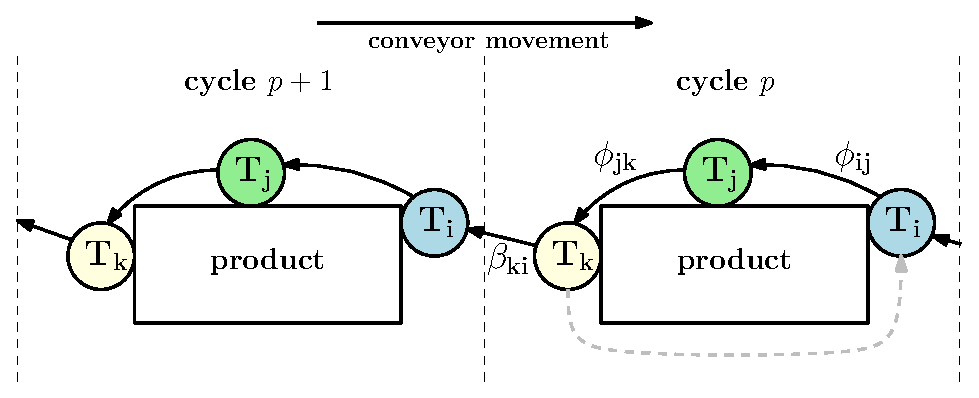
\includegraphics[width=0.8\textwidth]{images/IntroForwBackSetupEx.eps}
	\label{fig:intro:forwBackDifference}
\end{figure}

To see how these setups are differentiated, 
Figure \ref{fig:intro:forwBackDifference} depicts the sequence of tasks 
$T_i,\:T_j,\:T_k$ which are performed in a cyclic manner on consecutive
products.
The execution of tasks proceeds chronologically from right to left,
\ie $T_1$ is the first task performed in cycle $p$.
Forward setups arise between consecutive tasks operating
on the same product.
A backward setup cost is incurred between the last
task of cycle $p$ and the first task of the next cycle, $p+1$.
Each cycle begins at time zero with the execution of task $T_i$
taking $t_i$ time units to process.
Then after performing the forward setups $\phi_{ij}$ and $\phi_{jk}$
together with processing times $t_j$ and $t_k$,
the station operator must perform the necessary backward
setup operation before moving to the next
workpiece along the line. 
Thus, when including this backward setup time $\beta_{ki}$,
the following condition must be satisfied to have a 
feasible cycle time
$t_i+\phi_{ij}+t_j+\phi_{jk}+t_k+\beta_{ki} \leq c$.
In Figure \ref{fig:intro:forwBackDifference}, the gray arrow  from $T_k$ to $T_i$ implies
the cyclic nature of the sequence.

% Example \ref{ex:intro:simpleSetup} alters the previous
% example into an instance of the \sua{2}.

\begin{example}\label{ex:intro:simpleSetup}
	Again consider the instance from Example \ref{ex:intro:simple},
	but now with sequence-dependent setup times
	between tasks.
	The arrays of forward and backward setup costs
	can be found in Tables \ref{tab:intro:forwSetupTimes}
	and \ref{tab:intro:backSetupTimes} respectively.
	Note, that some of the entries in these arrays are
	omitted as the corresponding sequence of tasks is not 
	possible due to the precedence relations or
	logical restrictions.

	The previous optimal solution is amended
	to include the required setup costs and is given in Figure 
	\ref{fig:intro:exSchedSetupFeas}.
	Note that the setup cost of any task to itself is 
	defined as zero.
	% This results in a large forward setup, $\phi_{23}$,
	% occurring on station $S_2$.
	To reach the optimal solution we must now consider
	the sequence of tasks within each station.

	By moving task $T_3$ to station $S_3$ and considering
	the sequencing of $T_3$ and $T_4$, we find the optimal
	solution to this problem, given in Figure \ref{fig:intro:exSchedSetupOpt}.
	The optimal cycle time is 13 in this case.	\qed
\end{example}

\begin{table}[tpb]
	\centering
	\begin{minipage}{0.45\textwidth}
		\def\arraystretch{1.1}
		\centering
		\caption{Forward setup times}
		\vspace{2mm}
		\begin{tabular}{lllll}
			\toprule
			$\phi$ & $T_1$ & $T_2$ & $T_3$ & $T_4$ \\\midrule\midrule
			$T_1$ & -- & 3 & 3 & 3 \\
			$T_2$ & -- & -- & 2 & 3 \\
			$T_3$ & -- & -- & -- & 1 \\
			$T_4$ & -- & -- & 2 & -- \\
			\bottomrule
		\end{tabular}
		\label{tab:intro:forwSetupTimes}
	\end{minipage}
	\hfill
	\begin{minipage}{0.45\textwidth}
		\def\arraystretch{1.1}
		\centering
		\caption{Backward setup times}
		\vspace{2mm}
		\begin{tabular}{lllll}
			\toprule
			$\beta$ & $T_1$ & $T_2$ & $T_3$ & $T_4$ \\\midrule\midrule
			$T_1$ & 0 & -- & -- & -- \\
			$T_2$ & 3 & 0 & -- & -- \\
			$T_3$ & 3 & 5 & 0 & 3 \\
			$T_4$ & 3 & 3 & 1 & 0 \\
			\bottomrule
		\end{tabular}
		\label{tab:intro:backSetupTimes}
	\end{minipage}
\end{table}

\begin{figure}[tpb]
	\centering
	\begin{minipage}{0.47\textwidth}
		\centering
		\caption{Feasible solution with setup}
		\vspace{2mm}
		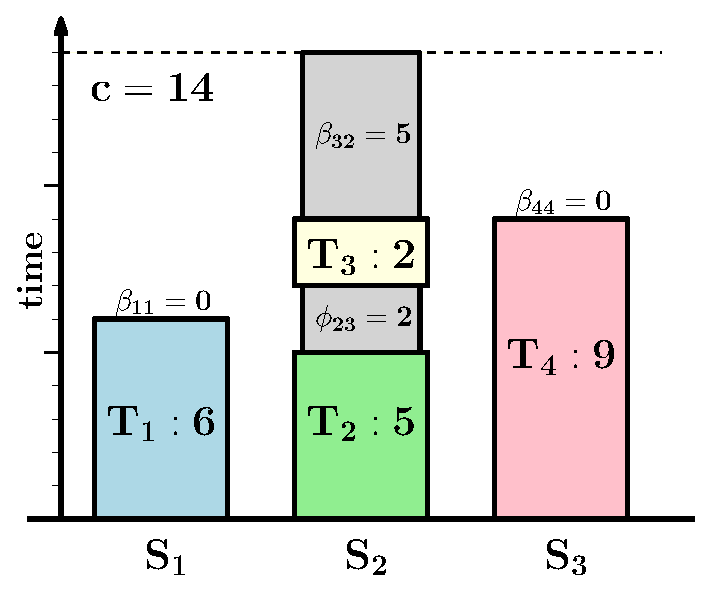
\includegraphics[width=\linewidth]{images/exSimpleSetupFeas.eps}
		\label{fig:intro:exSchedSetupFeas}
	\end{minipage}
	\hfill
	\begin{minipage}{0.47\textwidth}
		\centering
		\caption{Optimal solution with setup}
		\vspace{2mm}
		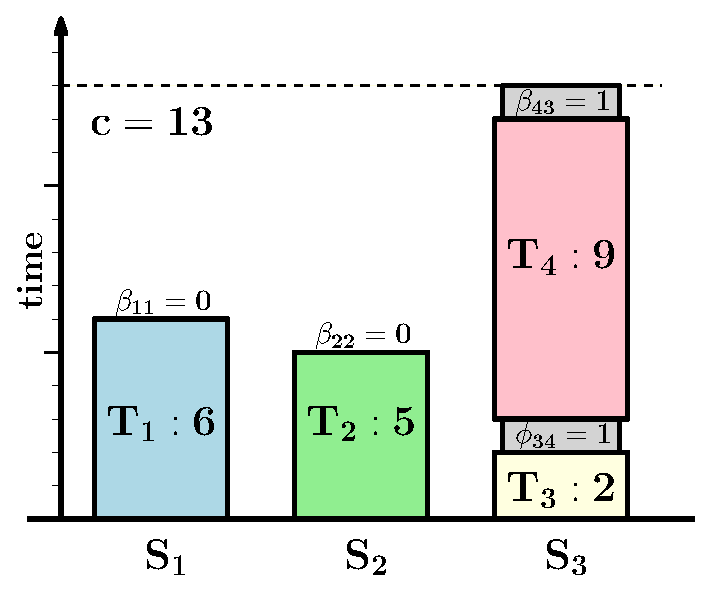
\includegraphics[width=\linewidth]{images/exSimpleSetupOpt.eps}
		\label{fig:intro:exSchedSetupOpt}
	\end{minipage}
\end{figure}

\section{Motivation}
\label{sec:intro:motiv}
In this section we provide motivation for why the \albp{}
with setup costs
is an important problem to be solved and why the approach we
chose to utilize is well-suited to the problem.

\subsection{Why the SUALBSP?}
Assembly lines were originally designed for the production
of a single type of product in high volumes.
Although, assembly lines able to produce only a single
product are not suitable for consumer-centric markets, 
where there is a need to tailor the products
more closely to the user's needs.
Sequence-dependent setup times are commonly considered
in job shop scheduling problems and a range of other
production problems (\cf \cite{Allahverdi2008a,Allahverdi2008b,Allahverdi2015}).
In those problems, the setup times arise because the products
are typically assumed to be highly diverse,
leading to additional configuration effort being required
between any two tasks.
In the context of operational planning of assembly lines,
sequence-dependent setup times have been sparsely
considered by the literature.
\authciteb{Scholl2013} list a number of possible
practical settings where setup times between tasks should not
be taken as negligible. Some include the following:
\begin{itemize}
	\item In automotive assembly lines where large workpieces (vehicles)
	need to be constructed, work can be performed at numerous
	mounting positions on the item.
	The size of the car body can result in walking distances
	between mounting positions being non-trivial.
	Thus, the preparation time (setup) can 
	be a critical aspect when sequencing the required tasks.
	\item Fixed material containers can be placed along the moving 
	conveyor system to allow workers to collect parts or tools needed.
	Further to walking times between these containers and the workpiece,
	the time taken to retrieve what is required from the container
	must also be accounted for.
	At a major German car manufacturer, these times contributed $10-15\%$
	of the total cycle time \cite{Scholl2013}.
	\item Specific tools are often required to perform a task.
	If consecutive tasks need different tools for their
	execution a tool-change between tasks will be necessary.
	Robotic assemblers used to perform the tasks of a station
	can be built to be highly flexible in the types of tasks
	they can perform.
	However, this flexibility can mean that numerous tool changes
	are required to switch from one task to another
	in a sequence.
	Thus, these sequence-dependent setup costs from tool-changes
	are typical in robotic assembly lines.
\end{itemize}
Consequently, accurately modelling the setup costs incurred
can be an important aspect when balancing an assembly line.

In practice, setup times are accounted for in simpler ways, such as
using an approximation or incorporating the setup time
into the task's processing time.
\citeauthor{Scholl2013} note that by using such approximations
``the planning team need to strike a fragile balance between an underestimation
of setups, which lead to infeasible line balances, and an overestimation
of setups, which leads to an allocation of excessive resources.''
The procedure used to estimate the cost of setups
can be time consuming and is prone to getting stuck in sub-optimal solutions.

For these reasons we feel that further research into the 
effect of setup times on the \albp{} is of interest to the
academic community and the manufacturing industry.

\subsection{Why Benders Decomposition?}
Benders decomposition is a well-known approach
to optimization problems.
It is naturally suited
to problems where the decisions can be separated into
two distinct sets.
Advances in the past few decades to the theory of
this method has broadened its applicability to a 
wider array of problems.
In our case, a solution to the \sua{2} can naturally
be divided into the assignment portion, which
assigns each task to a station, and the scheduling
portion, which decides on the time that each task
begins execution within a station.

We can view this separation of concerns in the following
way.
The manager of an assembly line needs a new item
to be put into production and so assigns the required
set of tasks to the stations along the line.
When calculating the line's cycle time the manager only estimates the setup times
within each station.
Each station operator must then decide if a possible sequencing
of their assigned tasks exists which can respect the manager's cycle time;
or if a precedence-feasible sequence exists at all.
% The worker at each station must then decide if there exists
% a possible sequencing of their assigned tasks which can
% respect the manager's cycle time; or if there a
% precedence-feasible sequence exists at all.
If at least one worker cannot find a feasible task-sequence
that respects the manager's cycle time
estimate, then a revision
may need to be made to the assignment of tasks.
The give-and-take between the assignment and scheduling portions
continues until a mutually satisfactory solution is found.
This informal process of communicating information between
the station workers and the assembly line manager could be time
consuming and not guarantee optimality.

The informal feedback loop between the two halves of the
decision problem suggests that Benders decomposition could be
employed to mimic this process.
The decision making process can naturally be divided
into a master problem, which assigns the tasks
to the stations along the line,
and several independent scheduling problems.
In total, there is a sub-problem
for each of the $m$ stations, which needs to
decide the exact execution time of all tasks
that station has been assigned.
Each sub-problem is similar to the asymmetric
Travelling Salesperson Problem (TSP)
with some forbidden paths due to the precedence
relations.
With this interpretation, the tasks are viewed as the 
cities and distances between them are the setup times.
To complete the iterative loop, the sub-problems
relay their information back to the master as
Benders cuts and the assignment problem is re-optimized.
In the words of J. N. Hooker,
``the Benders cuts added to the master problem are
the mathematical equivalent of telephone calls''
from the station workers to the line manager \cite{Hooker2007}.

The reader may be familiar with the classical version
of the Benders decomposition method due to the 
work of \authciteb{Benders1962} and \authciteb{Geoffrion1972},
however for the \sua{}, this approach is inappropriate.
Due to the sub-problems being highly-combinatorial discrete scheduling
problems, formulating them as a linear or non-linear program
will not be practical.
We instead explore how the more general method of \emph{logic-based}
Benders decomposition can be used to solve the \sua{2}.

By employing this approach we are able to exploit the comparative
advantages of multiple solving technologies to tackle each
portion of the problem.
Mixed-Integer Programs (MIPs) are well-suited to the assignment
problem of the master and Constraint Programming (CP), from 
the Computer Science discipline, is an effective solving technology
for scheduling problems.

\section{Problem Definition}
\label{sec:intro:probDef}
Here we present the core notation that will be used for the
remainder of the thesis.
Along the conveyor belt of the assembly line
there are \emph{work stations} $K=\{1,2,\ldots,m\}$.
Workpieces (or products/items) move down the 
conveyor belt from station to station.
A workpiece remains at each station for 
one cycle, which has a duration given by the \emph{cycle time}.
The objective of the \albp{} is to optimally partition
the total work required among the stations with respect to
a performance measure.

The work required to complete a single piece is separated into
a set of \emph{non-preemptive tasks} $V=\{1,2,\ldots,n\}$,
each with a discrete processing time $t_i$.
Physical and technical conditions impose a set of 
\emph{precedence relations} $E\subseteq V\times V$,
which prevent some non-allowed task orderings from occurring.
If we consider the graph $G=(V,E)$ with tasks as the vertex set
and directed edges defined by the precedence relations,
then $G$ is a directed acyclic graph (DAG).	
Without loss of generality, we may assume that the vertices
are numbered topologically so that the following holds:
$(i,j) \notin E$ if $i>j$.

Between each pair of tasks, discrete
\emph{forward} and \emph{backward setup} times
are predefined.
We denote the forward setup time between $i$ and $j$
by $\phi_{ij}$ and the backward setup time
by $\beta_{ij}$.
When $i=j$, the forward setup time is undefined
as a task can never follow itself in a station's
forward work load.
The backward setup $\beta_{ii}$, \ie the setup cost
of a task to itself, is defined as zero.

To fully specify a feasible solution to the \sua{2},
one must give the following:
an assignment of tasks to the stations
and the execution time window of each task within
its assigned station.
From this specification, the cycle time is calculated by
the total processing time of the station with the
largest workload.



%!TEX root = thesis-kdyoung.tex

\chapter{Theoretical Background} \label{chap:theory}
In this chapter we provide the theoretical background needed
for the work presented in the following chapters.
As such, we give summaries of the relevant literature from
four fields spanning mathematics and computer science.
These include background knowledge of the problem of assembly
line balancing (Sect. \ref{sec:lit:ALB}); modelling and solving technology from the areas
of linear programming (Sect. \ref{sec:lit:mip}) and constraint programming (Sect. \ref{sec:lit:cp});
and lastly we delve into some of the recent
advances into the theory of Benders decomposition (Sect. \ref{sec:lit:bend}).

\section{Assembly Line Balancing}
\label{sec:lit:ALB}
Optimizing the construction of an assembly line to maximize or minimize 
some performance measure has been a problem of great interest to the 
research community since its introduction by Henry Ford
in 1915 \cite{Ford1922}.
Simply, it can be stated as a decision problem
where we seek optimal partition of work to assemble
a product.
The work must be divided
among discrete stations along a line (\eg conveyor belt),
while respecting a series of restrictions imposed by physical
limitations.
All variants of the \albp{} begin from this common starting point
and add further restrictions or considerations which
results in a range of generalizations.
We refer the interested reader to one of the surveys
of \authciteb{Baybars1986},
\authciteb{Becker2006} or
\authciteb{Boysen2007} for a detailed snapshot of
the problem's various extensions.

In this section we detail the basic version of the 
problem and the particular variant which
is relevant to our work.

\subsection{Simple Assembly Line Balancing Problem}
\label{sec:lit:SALBP}
The Simple Assembly Line Balancing Problem is the basic
type of the \albp{} \cite{Baybars1986,Scholl1999}.
It consists of a serial production line which produces a 
single product.
The tasks which need to be executed to achieve a product's completion
all have fixed processing times and all stations
along the line are uniform, \ie each is equivalently equipped
and manned by homogeneous workers or machines.

There are two primary parameters of the assembly line
which dictate the aim when solving the problem; these parameters
are the \emph{cycle time} and the number of stations, denoted
by $c$ and $m$ respectively.
We denote the \emph{load} of station $k$ by $l_k$, which is
defined as the sum of all processing times of tasks assigned to station
$k$.
The cycle time of an assembly line is defined as follows,
\[
	c=\max\{ \: l_k \:|\: k \in K \:\},
\]
\ie the largest load among all stations.
Physically, the cycle time of an assembly
line can be interpreted as how much time each station is given to work on a product,
before the product moves to the next station.
A lower cycle time means the conveyor belt can move faster and
products are output at a higher rate.

From the parameters $c$ and $m$, the \albp{} can be formulated as three 
different but highly related problems: type-1, type-2 and
type-E.
We now summarize each variety and its particular qualities in turn,
\begin{itemize}
	\item Type-1: Fixed $c$, variable $m$.\\[1pt]
	The type-1 variety, abbreviated as \sab{1} in the simple case, considers the
	cycle time to be fixed and the number of stations to be decided.
	This most commonly occurs when constructing a new assembly line.
	As an example, the \sab{1} is characterized using the classification
	scheme of  \authciteb{Boysen2007} by $[-|-|m]$.
	\item Type-2: Variable $c$, fixed $m$.\\[1pt]
	For the type-2 variety, the aim is to find the optimal cycle time given 
	that the number of stations along the line is fixed.
	In practice, this variety commonly corresponds to adapting an existing assembly line
	for a new purpose.
	\item Type-E: Variable $c$, variable $m$.\\[1pt]
	This variety deals with the case when both $c$ and $m$ are considered
	to be decision variables of the problem. Here, the objective
	is to optimize some measurement of line efficiency.
\end{itemize}

\subsection{Setup Assembly Line Balancing and Scheduling Problem}
\label{sec:lit:SUALBSP}
In this document, we are concerned with the SetUp Assembly Line Balancing and Scheduling Problem.
This variant differs from the basic \sab{} by introducing
sequence-dependent setup times between pairs of tasks
within a station's workload.
This type of consideration was first made in the literature by \authciteb{Andres2008}
in an attempt to reduce the gap between the existing academic theory
and the realities of assembly line problems posed by the industry.
In the problem tackled by \citeauthor{Andres2008},
they considered a setup time to exist between
a pair of consecutive tasks inside a station's sequence.
As such, it needed to be added to that station's
global processing time
and so these setup times directly affected
the cycle time of the line.
The authors considered heuristic rules and employed a Greedy
Randomized Adaptive Search Procedure (\grasp) to tackle the
type-1 version of the problem.
They also developed a lower-bound which was used
to estimate the quality of their solutions found.

Later, some of the same authors continued this work in
\authciteb{Martino2010}, where over 50 priority-rules were considered
for a heuristic procedure designed for the type-1 version.
All results found for the problem at this point in the 
literature indicated that adding these sequencing considerations
for the tasks made the problem much more difficult to solve.
This is demonstrated by only very small instances of the problem
being able to be optimally solved.

More recently, the work of \authciteb{Scholl2013} extended the previous
work on this problem and formally named it the \sua{}.
The \sua{} differs slightly from the problem tackled previously
by introducing a distinguishment between \emph{forward} and \emph{backward}
setup times.
The motivation for this differentiation is so the theoretical
problem can more accurately capture the physical aspects
of sequencing tasks.
A forward setup time occurs between two consecutive tasks assigned the same station,
if each task is processing the same item.
A backward setup time occurs between two consecutive tasks assigned the same station,
if each task is operating on different items on the assembly line.
Physically, a backward setup time captures the setup cost between the last task on the current
product and the first task on the next product.
We demonstrate this idea using 
a possible task sequence within two stations in Figure \ref{fig:lit:forwBackSetupExAbstractB}.
Forward setup times are denoted by $\phi$ and backward setup times
by $\beta$.

% \begin{figure}[H]
% 	\centering
% 	\caption{Setup times of a station's sequence (test A)}
% 	\vspace{2mm}
% 	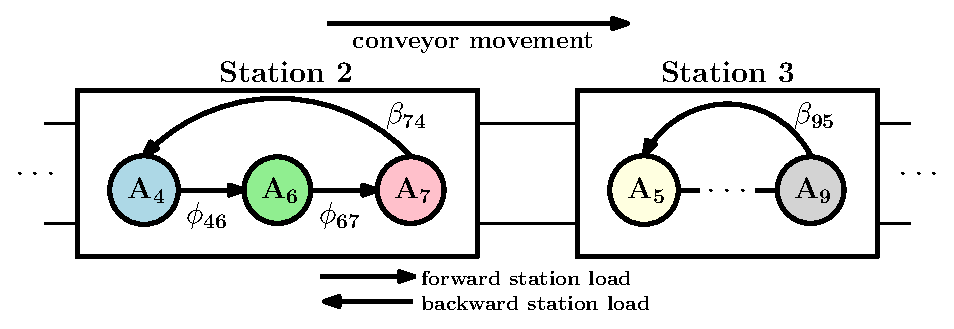
\includegraphics[width=0.9\textwidth]{images/forwBackSetupExA.eps}
% 	\label{fig:lit:forwBackSetupExAbstractA}
% \end{figure}

\begin{figure}[tpb]
	\centering
	\caption{Setup times of a station's sequence}
	\vspace{2mm}
	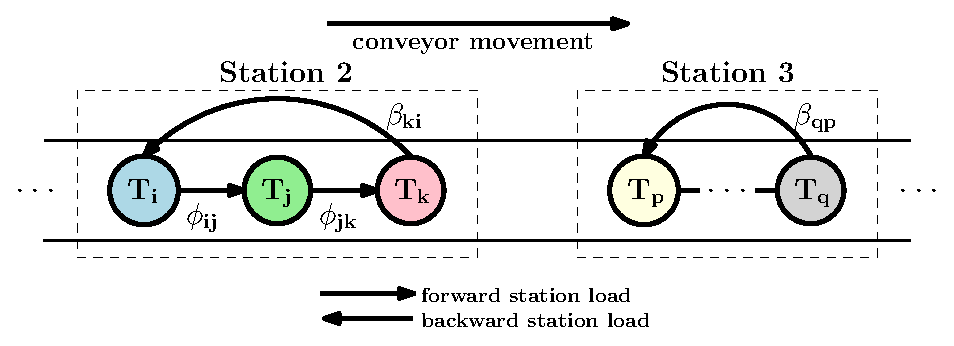
\includegraphics[width=0.9\textwidth]{images/forwBackSetupExB.eps}
	\label{fig:lit:forwBackSetupExAbstractB}
\end{figure}

% \begin{figure}[H]
% 	\centering
% 	\caption{Setup times of a station's sequence (test C)}
% 	\vspace{2mm}
% 	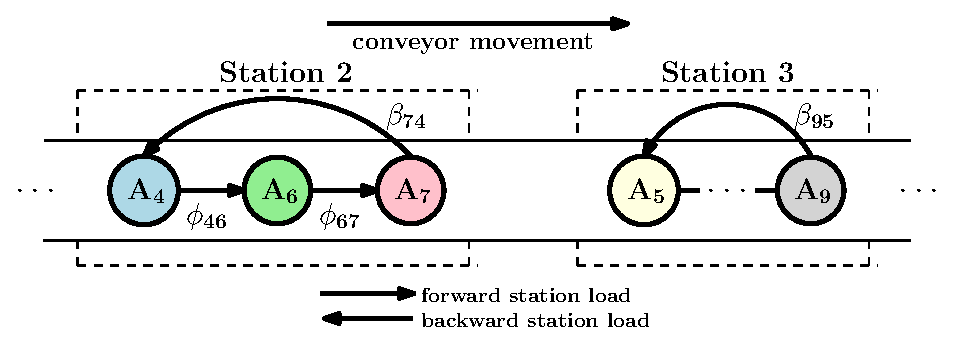
\includegraphics[width=0.9\textwidth]{images/forwBackSetupExC.eps}
% 	\label{fig:lit:forwBackSetupExAbstractC}
% \end{figure}

\authciteb{Scholl2013} proposed an exact solution approach by a
mathematical formulation of the type-1 problem as a mixed integer program.
Using the scheme of \authciteb{Boysen2007},
the \sua{1} can be formally classified as,
\[	\text{\sua{1}: }[\Delta t_{dir}|-|m].	\]
Further to their mathematical model, a range of tools were proposed which could be composed
in a number of ways to create new heuristic approaches for the problem.

\authciteb{Esmaeilbeigi2016} give the most recent contribution of the literature
to the study of the \sua{}.
In their paper, three new mixed-integer formulations are presented of the \sua{1}
which are based on different ways of representing the decisions.
Their first two formulations are station-based and the last is a purely
scheduling-based formulation which has abstracted the
assignment decisions away from the problem.
Each of the three models presented are also modified to be suited
to the type-2 version of the \sua{}.
Although these models were presented, the type-2 problem
was not the authors primary concern and as such the models were not tested.

In the literature there have been few attempts to tackle the type-2 variety of the \sua{}.
The first was by \authciteb{Yolmeh2012} who use a Genetic Algorithm
which is applicable to either the type-1 case or type-2 case.
The only other approaches to the type-2 problem
which have been explored are the three mixed integer programs
mentioned earlier from \authciteb{Esmaeilbeigi2016}.

\section{Mixed Integer Programming}
\label{sec:lit:mip}
A Mixed Integer Program is a common extension of the fundamental
Linear Program (LP) of the Operations Research discipline.
MIPs present the additional constraint on some of their decision
variables that restrict their domain to exclusively integer values.
Problems which require integer valued solutions occur in many
real-world scenarios.
Example \ref{ex:lit:simpleMIP} presents a simple but quite
useful application of a problem with integer variables.

\begin{example}\label{ex:lit:simpleMIP}
	Consider assigning staff members to complete
	a given set of tasks.
	For a solution of this problem to be feasible we require that
	no fraction of any staff member is split across multiple tasks.
	Using continuous variables to model
	this problem will lead to invalid solutions and thus integer-valued
	variables are required. \qed
\end{example}

The flexibility of the mixed integer programming approach to modelling
problems has allowed MIPs to model a wide-range of optimization
problems.
A typical solution methodology when approaching a MIP is to
consider its linear relaxation.
This presents a much simpler problem to solve, but 
recovering a feasible integer solution from this relaxed problem
can prove challenging.

\subsection{Branch and Bound}
\label{sec:lit:mipBB}
The Branch and Bound (\bab) algorithm is a general tool which can
be applied to solve optimization problems which was first proposed by \authciteb{land1960}.
The structure of the method is general enough that it can be used
as a design paradigm for more involved ways of exploring the
solution space. As a result, it has spawned 
a variety of adaptations in the field of operations research since its
inception. Some of these include branch-and-cut (\authcite{Padberg1991}),
branch-and-price (\authcite{Savelsbergh1997})
and branch-and-infer (\authcite{Bockmayr1998}).
A procedure based on the \bab algorithm is the typical way of
approaching MIPs and so we now give an overview of
how this method operates.

The \bab method constructs a rooted tree used to explore the set of
all feasible solutions.
At a node of the tree, a decision variable is chosen as
the branching variable and the domain
of possible values for that variable is divided
between two child nodes.
The solution space of the current node is split
into two smaller disjoint subsets in these child nodes.
At the root of the tree, the solution space corresponds to all
possible feasible solutions to the original LP relaxation of the problem.
For each new node created by branching, the corresponding
relaxed LP is solved to determine the optimal
value at each node.
When each node is processed, a procedure called \emph{fathoming},
its optimal value is checked for both
integrality and feasibility.
If the node's solution is optimal and integer then it is compared to
the current best integer solution.
In a minimization (maximization) problem, if the new solution 
is less (more) than the current best, then 
the current best is replaced with the new optimal integer solution.
This new solution is called the incumbent.
Branching on the feasible solution space and solving each
relaxed sub-problems continues until all branches have been either
explored or are deemed unnecessary to explore, \ie \emph{pruned}.
At termination, the current incumbent solution is the optimal solution
to the original non-relaxed MIP, and thus the original problem
is solved.
We provide some pseudo-code of the \bab algorithm
for a minimization MIP in Algorithm \ref{alg:lit:bab}
in the Appendices.

\subsection{MIP Solver: \gurobi}
\label{sec:lit:mipGurobi}
\gurobi is a commercial solver designed for mathematical optimization problems including
LPs, quadratic programs (QPs) and MIPs.
Significant advances have been made to Gurobi's capabilities and other MIP solvers
during the last few decades due to a number of improvements
in the theory and computational hardware available \cite{Bixby2002}.
Some of the most important improvements in this area
are detailed in \authciteb{Lodi2010}.
These factors have given MIP solvers the ability to 
solve highly complex optimization problems while providing
a relatively easy to use interface for doing so.

To solve a MIP, Gurobi uses the branch-and-cut version
of the \bab algorithm.
Preprocessing is a common procedure implemented by solvers
where the problem's input to the solver is altered 
to remove obviously sub-optimal solutions from 
the solution space without removing any possibly optimal solution.
Further to this pre-solving step, there are numerous 
improvements made to the procedure of the \bab also.
Additional constraints called \emph{cutting planes}, or
simply \emph{cuts}, are added to the model
which do not remove any feasible solution but result in the linear relaxation
being closer to the non-relaxed problem's feasible solution space.
The feasible solution space of the original problem is
called the \emph{convex hull}.

Advances in the hardware over the past few decades
has been the other main source of improvement to solvers such as Gurobi.
Utilizing an algorithm which depends on branching the solution space
into disjoint subsets, has naturally favoured solvers such as Gurobi
by allowing them to take full advantage of parallel computing.
Currently, \gurobi can concurrently solve 1024 branches of
a \bab tree.
Taking advantage of this parallelization can provide
more than just a 1024-fold increase is computational power
due to the communication of solutions between branches.
For example, if one branch finds a high-quality integer feasible solution
then all other branches can immediately reap the benefits
by getting access to more effective pruning.

\section{Constraint Programming}
\label{sec:lit:cp}
Constraint Programming (CP) is a framework for modelling and solving optimization problems.
This framework has its roots in the field of Artificial Intelligence and the initial
conception of the idea is due to \authciteb{Jaffar1987},
who pointed out that the language PROLOG II is a special
case of a more general scheme: Constraint Logic Programming. 
CP uses a declarative descriptive of the problem by defining a set of decision variables
each with a set of possible values, \ie domains;
and a set of constraints which restrict the possible combinations of values for the
decision variables.

Over the past two decades, CP has been used extensively
to tackle a variety of combinatorial optimization problems.
The success of constraint programming can generally be attributed
to two of its unique features
\begin{enumerate}
	\item \emph{heterogeneous global constraints} which allow the user to write a high level
	model using the global constraints to capture important combinatorial structures.
	In most cases these constraints are formulated in such a way to be abstracted 
	away from the specific properties of any one problem.
	\item \emph{user-defined search} which allows the user to specify a structured
	search procedure for exploring the solution space, using their familiarity
	with the problem.
\end{enumerate}

CP has proven itself to be an effective solving technology
for many scheduling problems such as project \cite{Berthold2010}, 
train \cite{Rodriguez2007} and 
employee scheduling \cite{Demassey2005}
as well as other types of combinatorial problems such as bin packing \cite{Pisinger2007}.

We now provide short explanations of the features of CP mentioned above
and a description of the CP solver we chose to use, \chuffed.
To communicate with the solver, we chose to write our constraint
programs using the solver-independent CP language 
MiniZinc \cite{Nethercote2007}.
MiniZinc provides a vast library of global constraints
as well as an adequate search language.

\subsection{Global Constraints}
\label{sec:lit:cpGlob}
Global constraints are one of the powerful tools made available to us
when formulating constraint programs. They allow us to succinctly encode
complicated combinatorial structures that commonly occur among
discrete problems. One of the simpler, 
but highly applicable, global constraints is given in
Example \ref{ex:globCons}.

\begin{example}\label{ex:globCons}
	\aldif is a global constraint that takes an array of integer
	variables, each with a possibly different domain of possible values. This constraint
	simply requires all given variables to take different values in the solution. \qed
\end{example}

One drawback of global constraints is that each one must be individually
implemented in the solver. When posed by a problem with inherent combinatorial
structures, your choice of solver can be restricted as some solvers may
only partially support, or not support at all, the needed global constraints.
However the benefits of this type of constraint are not to be understated.
The fact that global constraints are formulated to be problem-agnostic can
provide users with much easier access to advances in the state-of-the-art solving technology.
To illustrate this point we consider the global constraint \cumu.

The \cumu global constraint was first introduced by \authciteb{Aggoun1993}
to efficiently solve and succinctly model a complex scheduling
problem.
Since then, the \cumu constraint has been widely used in a variety of problems
due to the fact that resources which are cumulatively restricted occur in many real-world problems.
A cumulatively restricted resource could represent a limited work force needed to execute a set
of tasks or a machine with a restriction on the number
of tasks it can run in parallel \cite{Schutt2011a}.

The \cumu constraint has commonly been applied to the Resource Constrained
Project Scheduling Problem (\RCPSP), which has many variants that 
are well-disposed to utilize the benefits of this global constraint.
Since its introduction, the \cumu constraint has had a number of improvements
proposed, some of these were by \authciteb{Caseau1994}, \authciteb{Nuijten1994},
\authciteb{Baptiste2000} and \authciteb{Carlier2004}. Each time an improvement
is made to \cumu~--- either by strengthening its propagation or by allowing it
to capture more varied and complex structures --- the results of all
problems where \cumu has previously been applied are improved as well.

% \begin{figure}[tbp]
% 	\centering
% 	\caption{Example of \cumu applied to a small cumulative resource problem {\color{red} (not complete)}}
% 	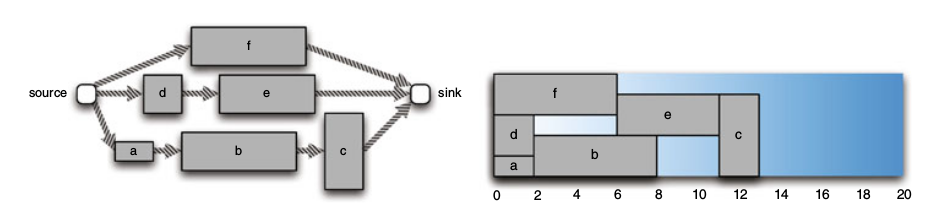
\includegraphics[width=0.95\textwidth]{images/cumu.png}
% 	\label{fig:examplePrecGraph}
% \end{figure}

By encoding the combinatorial nature of a problem using the global
constraints made available to us by CP, we are able to not
only take advantage of all the previous theoretical improvements to a global
constraint, but all future advances as well.

\subsection{User-Defined Search Procedures}
\label{sec:lit:cpSearch}
MiniZinc is a powerful modelling language for constraint programming
which is capable of concisely specifying complex models.
One of the reasons it was the language we chose to write
our constraint programs with was its ability to define relatively
structured search procedures with ease \cite{Schrijvers2013a,Schrijvers2013b,VanHentenryck2000}.

The current search facilities provided by MiniZinc can be 
separated into two types: basic searches and compositional searches.
To demonstrate the features of a basic search we present
a simplification of MiniZinc code here in 
Listing \ref{lst:intsearch}. This basic search specifies a
search procedure over an integer variable, namely \intser,
\begin{lstlisting}[caption={Basic integer search procedure},label={lst:intsearch},language=minizinc]
int_search(array[int] of var int, ann, ann);
\end{lstlisting}\vspace{5mm}

The declaration of the basic integer search, requires 3 inputs to fully
define how it divides the set of feasible solutions
and chooses which variables to branch on. Let the declaration be defined by input 
$(x,varselect,varsplit)$. The decisions variables which need to have 
their values fixed are given by $x$. The annotation $varselect$ specifies
the order in which to select the variables depending on some selection criteria.
Lastly, $varsplit$ defines how to branch on the chosen variable's 
possible values. During this branching process, variables which have their
domains reduced to a singleton value are fixed and removed from
later consideration.

There are many variable selection strategies which MiniZinc's search language
offers. The simplest selection criterion is {\tt input\_order} which selects
the variables in the order given.
Some of the possible selection criteria which
are offered by MiniZinc are presented in Table \ref{tab:selectCrit}.

MiniZinc also offers a multitude of value splitting methods to allow
the user to specify application tailored branching strategies.
The branching of any search procedure is characterized by
creating one branch satisfying the specified splitting
property and another branch satisfying its negation.
For example, using the splitting method {\tt indomain\_min}
will create one branch in the search tree where the chosen variable's
domain is reduced to its minimum value --- \ie this variable is fixed
--- and another branch where the minimum value of the variable
is removed from the domain.
Some of the possible branching methods MiniZinc
has implemented are presented in Table \ref{tab:valueSplit}.
Example \ref{ex:lit:basicSearch} presents a simple
use of the \intser procedure on an array of integer
variables.

\begin{table}[tpb]
	\def\arraystretch{1.2}
	\centering
	\caption{Examples of MiniZinc's variable selection criteria}
	\vspace{2mm}
	\begin{tabular}{p{0.25\textwidth}p{0.65\textwidth}}
		\toprule
		Selection Criteria & Definition \\
		\midrule\midrule
		{\tt input\_order} & Choose variables in the order given \\
		{\tt smallest} & Choose the variables with the smallest possible value in their domain \\
		{\tt smallest\_largest} & Choose the variables with the smallest largest possible value in their domain \\
		{\tt first\_fail} & Choose the variables with the smallest domain \\
		\bottomrule
	\end{tabular}
	\label{tab:selectCrit}

	\caption{Examples of MiniZinc's variable splitting methods}
	\vspace{2mm}
	\begin{tabular}{p{0.25\textwidth}p{0.65\textwidth}}
		\toprule
		Variable Splitting & Definition \\
		\midrule\midrule
		{\tt indomain\_min} & Branch on the minimum value of the chosen variable \\
		{\tt indomain\_max} & Branch on the maximum value of the chosen variable \\
		{\tt indomain\_random} & Branch on a random value in the  chosen variable's domain \\
		{\tt indomain\_split} & Branch on the chosen variable such that the domain is split in half \\
		\bottomrule
	\end{tabular}
	\label{tab:valueSplit}
\end{table}

\begin{example}\label{ex:lit:basicSearch}
	For example, consider a search annotation 
	$${\tt int\_search([x,y,z],~smallest,~indomain\_min)},$$
	with current domains of the variables $x\in\{5\},\:y\in\{7,\ldots,12\},\:z\in\{2,\ldots,9\}$.
	As we have the {\tt smallest} variable selection strategy, the variable $z$ will be chosen
	as the branching variable. Using {\tt indomain\_min} will result in one branch were $z$'s value
	is fixed to 2 and another branch where its domain is reduced to $\{3,\ldots,9\}$. \qed
\end{example}

Further to the search strategy for arrays of integer variables, MiniZinc also has
similar search structures available for arrays of boolean variables ({\tt bool\_search}) and 
arrays of float variables ({\tt float\_search}).

The most important feature in MiniZinc's search language is its ability to compose
primitive searches to create complex application-tailored search procedures.
This is done through the use of search combinators developed in \cite{Schrijvers2013b}
and \cite{Schrijvers2013a}.
We briefly detail here how MiniZinc's sequential search
combinator, {\tt seq\_search}, can be used. MiniZinc's sequential search definition
is given in Listing \ref{lst:seqsearch} and we show how it
can be used in Example \ref{ex:lit:seqSearch}.

\begin{lstlisting}[caption={Sequential search procedure},label={lst:seqsearch},language=minizinc]
seq_search(array[int] of ann);
\end{lstlisting}\vspace{5mm}

\begin{example}\label{ex:lit:seqSearch}
	Consider the sequential search annotation in Listing \ref{lst:seqsearchEx},
	which first will decide all boolean variables $b1,\:\ldots,\:b3$, by branching on
	a random variable in each one's domain.
	After all boolean variables are fixed, the procedure will search over
	possible values for the $x$ variables choosing to branch on the one with the smallest value in its domain. \qed
\end{example}
\begin{lstlisting}[caption={Example of a sequential search annotation},label={lst:seqsearchEx},language=minizinc]
seq_search( [bool_search([b1,b2,b3], input_order, indomain_random), 
             int_search( [x1,x2,x3], smallest,    indomain_min)    ] );
\end{lstlisting}\vspace{5mm}

Later in Section \ref{sec:bend:cpSearch}, we formulate specific
search strategies to effectively tackle our problem.
To achieve this, we will provide 
a more in-depth look into some of the recent developments in
MiniZinc's search language and how we have employed them.

\subsection{CP Solver: \chuffed}
\label{sec:lit:cpChuffed}
To solve the constraint programs that arise in our solution 
methodology, we chose to use the CP solver \chuffed which
was initially developed in the Ph.D thesis of \authciteb{Chu2011}.
In this section we will note the advantages that this solver
provides and also the solver's drawbacks.

What sets \chuffed apart from other competing CP solvers 
are its two main features:
lazy clause generation (\LCG) and boolean satisfiability solving (\SAT).
Since the introduction of \LCG to solving technology, CP solvers
which have integrated it into their procedures
have become very well suited to scheduling problems \cite{Ohrimenko2009}.
Their ability to learn nogood clauses 
has allowed this type of solver to effectively prune the search space,
using conflict-driven search to guide the branching strategy \cite{Szeredi2016,Schutt2015,Schutt2011b,Schutt2013b}.

An important feature of CP solvers is their Finite Domain (FD) propagation.
A propagator can be thought of as an `explanation' of a truth. Generally
this can be represented by $a_1\wedge a_2 \wedge \ldots\wedge a_n \rightarrow d$,
where each $a_i$ represents an existing domain restriction and $d$ represents
the implied domain restriction. This is demonstrated by Example \ref{ex:lit:domProp}.
CP solvers which have access to \SAT solving technology extend their ability
to use FD propagation on clauses of literals, rather
than being restricted to propagation of variable domains.
\begin{example}\label{ex:lit:domProp}
	Suppose our problem has three decision variables with domains
	$x\in\{3,10\}$, $y\in\{2,10\}$ and $z\in\{0,10\}$. Given the constraint
	$z\geq x+y$, we can use finite domain propagation to add the following
	propagator to our model $(x\geq3)\wedge(y\geq2) \rightarrow (z\geq5)$.\qed
\end{example}

Later in Section \ref{sec:bend:cpGlob}, we make use of
the global constraint \cumu to encode some of the combinatorial
nature of our problem.
Recent additions in the propagation qualities of \cumu, such as
time-table filtering \cite{Schutt2011a} and 
time-table-edge-finding filtering \cite{Schutt2013c},
are all readily available in \chuffed.

The final advantage of \chuffed is that all
search capabilities offered by the language MiniZinc
have been fully implemented.
Perhaps most importantly, \chuffed
is the only available solver that supports a recent
addition to MiniZinc's search language,
which will be detailed further in Section \ref{sec:bend:cpPriSearch}.
This together with our familiarity with \chuffed and 
it being a state-of-the-art solver for numerous scheduling
problems, which are closely related to the constraint programs we encountered,
made it the obvious choice of solver.

One significant disadvantage of \chuffed which must be mentioned,
is its inability to be run in parallel.
The most common way to 
parallelize CP solvers is by splitting the search space into disjoint
subspaces and running independently on each branch.
Although \chuffed being a \LCG solver with nogood learning has presented some unique
difficulties in achieving an effective parallelization.
Communicating learnt clauses  between parallel solvers is advantageous to reduce 
the amount of repeated work, but the ability to communicate complex clauses is quite limited.
Recent work by \authciteb{Ehlers2016} has shown that it is
possible to achieve an effective parallelization of \chuffed, 
but unfortunately this technology is still in development and
we were not able to make use of it for our computational tests.

\section{Benders Decomposition}
\label{sec:lit:bend}
Benders decomposition is a method for solving optimization problems
which was original proposed in the seminal paper
by J. F. Benders in \citeyear{Benders1962}.
The method is loosely based on the notion of
``learning from one's mistakes'';
which is achieved through intelligently
partitioning the problem and delayed constraint generation.
This approach is well-suited to problems where the
decision variables can be divided into a set of primary
and secondary decisions.
When the secondary variables, also called \emph{complicating} variables,
are fixed the original problem becomes substantially
simpler to solve.
Fixing the complicating variables either partitions the problem
into two easier problems, namely the \emph{master}
and the \emph{sub-problem}, or results in such a structure
where the solution is straightforward.
This idea is demonstrated in the following linear program,
\begin{IEEEeqnarray}{RcRcRcRCl}
	\IEEEeqnarraymulticol{9}{c}{\text{Min }~ x_1+x_2+x_3 ~{\color{red} +~y}}  \label{eq:lit:compVars1}\nonumber\\[\eqnv]
	\text{subject to }\quad 2 x_1 &\hspace{1mm}& +~x_2 &\hspace{1mm}& &\hspace{1mm}& {\color{red} +~3y} &\geq& 8  \label{eq:lit:compVars2}\nonumber\\[\eqnv]
	 &\hspace{1mm}& x_2 &\hspace{1mm}& -~2x_3 &\hspace{1mm}& {\color{red} -~2 y} &\geq& 3  \label{eq:lit:compVars3}\nonumber\\[\eqnv]
	 &\hspace{1mm}& &\hspace{1mm}& x_3 &\hspace{1mm}& {\color{red} +~7 y}  &\geq& 2.  \label{eq:lit:compVars4}\nonumber
\end{IEEEeqnarray}
We have a set of complicating variables, $y$,
occurring in all constraints
and a set of primary variables, $x$, whose solution would be straightforward
if $y$ were fixed.

% \begin{figure}[tbp]
% 	\centering
% 	\caption{Simple example of complicating variables in a LP {\color{red} (not complete)}}
% 	\label{fig:lit:compVarsEx}
% 	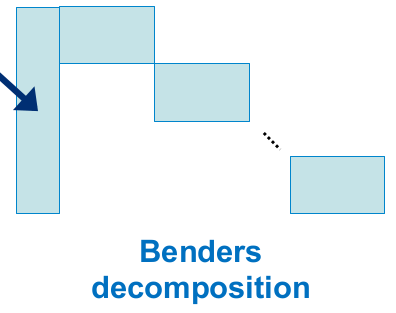
\includegraphics[width=0.5\textwidth]{images/compVarsExample.png}
% \end{figure}

Once the problem is divided into the master and sub-problems, the 
Benders algorithm iterates between them; solving each one in turn and uses
these solutions to gradually learn where the most
important infeasibilities of the problem exist.
A top-level view of how the Benders decomposition procedure
iterates is given in Figure \ref{fig:lit:topLevelBenders}.
In the case of minimization, the solution to the relaxed master 
problem, or RMP, provides a lower bound on the optimal value.
This trial solution of the RMP is then passed to the sub-problem
and, if possible, the sub-problem is solved to optimality.
If the solution to the sub-problem is infeasible or sub-optimal,
we find out why and then use this information to design
a constraint to pass back to the master, which will rule out
the current trial solution.
This constraint is called a \emph{Benders cut}.
It is preferable
to formulate these cuts such that not only the current trial solution
is removed from the relaxed master's feasible region, but also
a large class of other solutions which are infeasible/sub-optimal for
similar reasons.

\begin{figure}[tbp]
	\centering
	\caption{High level structure of the Benders decomposition method}
	\vspace{2mm}
	\label{fig:lit:topLevelBenders}
	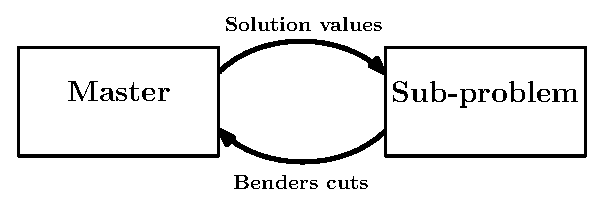
\includegraphics[width=0.6\textwidth]{images/bendersAbstract.eps}
\end{figure}

Since its introduction by \citeauthor{Benders1962},
this approach has been generalized to be applicable to a wider range of problem
structures. We now provide a review of the classical version of the method
as well as some of its recent adaptations.

\subsection{Classical Benders}
\label{sec:lit:clasBend}
The initial decomposition method proposed by \citeauthor{Benders1962}
was used to find the solutions of MIPs via partitioning
the problem into two simpler linear programs.
We refer the interested reader to the surveys by
\authciteb{Costa2005} and \authciteb{Rahmaniani2017}.
We now present how this decomposition could be applied
to a general minimization problem, based on the work
of \authciteb{Saharidis2010}.

Consider a problem where the set of decision variables
can be divided into two sets, $x$ and $y$, where
$y$ is a set of complicating variables.
The problem can be modelled by the following program
\begin{IEEEeqnarray}{rCl}
	\IEEEeqnarraymulticol{3}{c}{\text{Min }~ c^T x+d^T y}  \label{eq:lit:bendSimple1}\\[\eqnv]
	\text{s.t. }\quad Ax+By &\leq& b  \label{eq:lit:bendSimple2}\\[\eqnv]
	Fy &\leq& p    \label{eq:lit:bendSimple3}
\end{IEEEeqnarray}
By applying Benders decomposition here we receive
two simpler problems: a master deciding the $y$ variables with
all constraints involving $y$,
and a sub-problem deciding the $x$ variables with all
constraints involving $x$.
So by considering a trial solution, $y=\bar{y}$, of the complicating variables,
we can pass this information to the sub-problem
which is formulated as follow,
\begin{IEEEeqnarray}{rCl}
	\IEEEeqnarraymulticol{3}{c}{\text{Min }~ c^T x+d^T \bar{y}}  \label{eq:lit:bendSP1}\\[\eqnv]
	\text{s.t. }\quad Ax &\leq& b - B\bar{y}  \label{eq:lit:bendSP2}
\end{IEEEeqnarray}
Using the duality properties of LPs we can instead consider the
dual variables $u$ and represent this sub-problem by its dual as follows,
\begin{IEEEeqnarray}{rCl}
	\IEEEeqnarraymulticol{3}{c}{\text{Max }~ (b-B\bar{y})u } \label{eq:lit:bendSPdual1}\\[\eqnv]
	\text{s.t. }\quad A^T u &\leq& c  \label{eq:lit:bendSPdual2}
\end{IEEEeqnarray}
This is the sub-problem which is solved to optimality or
proven infeasible.
The objective function of the sub-problem varies with
$y$ but the feasible set of solutions is independent
of these complicating variables.

If the solution of the master problem is feasible
then the dual of the sub-problem will find optimality at 
an extreme point, while if the master's solution was
infeasible, the sub-problem is unbounded indicating the
existence of an extreme ray in its solution space.
In either case, we can formulate a Benders cut to add
back into the master problem to remove the current solution
from the feasible set.

When the sub-problem's solution is bounded and optimal
we can add what are called \emph{optimality} cuts to the master problem
\begin{IEEEeqnarray}{rCl}
	z&\geq& (b-By)\bar{u}_i^T + d^T y,\quad i=1,2,\ldots \label{eq:lit:bendExtPt}
\end{IEEEeqnarray}
where each $u_i$ corresponds to an extreme point. When the solution is unbounded
we can create \emph{feasibility} cuts for each extreme ray
\begin{IEEEeqnarray}{rCl}
	(b-By)\bar{v}_j^T &\leq& 0,\quad j=1,2,\ldots \label{eq:lit:bendExtRay}
\end{IEEEeqnarray}
where each $v_j$ corresponds to an extreme ray. After these cuts are created
we add them into the master problem and re-solve to find a new trial solution
for $y$. The new RMP is formulated as follows
\begin{IEEEeqnarray}{rClCl}
	\IEEEeqnarraymulticol{3}{c}{\text{Min }~ z} &\hspace{4mm}& \label{eq:lit:bendSimpleMast1}\\[\eqnv]
	\text{s.t. }\quad Fy &\leq& p & & \label{eq:lit:bendSimpleMast2}\\[\eqnv]
	z &\geq& (b-By)\bar{u}_i^T + d^T y & & i=1,2,\ldots   \label{eq:lit:bendSimpleMast3}\\[\eqnv]
	(b-By)\bar{v}_c^T &\leq& 0 & & j=1,2,\ldots   \label{eq:lit:bendSimpleMast4}
\end{IEEEeqnarray}

\authciteb{Geoffrion1972} generalized the classical approach to a broader class
of optimization problems which meant the sub-problems no longer needed
to be formulated as a linear program but could also be nonlinear.
Further to this improvement, \authciteb{Magnanti1981} investigated 
ways to generate Pareto-optimal Benders cuts to produce a tighter
relaxation in the master problem.
Other possible enhancement methods for Benders decomposition
exist including two- and three-phase heuristic approaches devised by \authciteb{Cordeau2001};
trust regions to significantly reduce the runtime considered by \authciteb{Santoso2005}
and \authciteb{Maher2014};
and parallelized solving of the decomposed problem studied by \authciteb{Dempster1998}
and \authciteb{Nielsen1997}.

\subsection{Logic-Based Benders}
\label{sec:lit:logicBend}
\citeauthor{Hooker2003}'s seminal paper from \citeyear{Hooker2003}
propose another generalization of Benders decomposition
to a much wider context while maintaining the strategy of
``learning from ones mistakes''.
One of the central ingredients in Benders decomposition
is the Benders cuts which allow information to be
communicated between the partitions of the problem.
In the classical case, the formulation of the sub-problems
is restricted to linear and non-linear programs.
However, this requirement hinders the ability of
Benders decomposition to be applied to problems
which are highly combinatorial in nature, such as scheduling,
as it can be impractical to formulate combinatorial problems
using a linear or non-linear model.

\citeauthor{Hooker2003} note that ``the key to generalizing Benders decomposition
is to extend the class of problems for which a suitable dual can be formulated''.
To this end, they introduced the concept of an \emph{inference dual} of any
optimization problem to the literature.
We note that this dual is different to the traditional LP dual
that the reader my be familiar with.
The inference dual is a proof of optimality which allows us to formulate
Benders cuts purely through logical reasoning.
This adaptation of the classical method proposed in \cite{Benders1962}
is named \emph{logic-based} Benders decomposition.

A formal description of logic-based Benders decomposition
applied to a minimization problem, based on the work
of \authciteb{Hooker2007}, is presented as follows.

Logic-based Benders decomposition applies to problems of the form
\begin{IEEEeqnarray}{rCl}
	\IEEEeqnarraymulticol{3}{c}{\text{Min }~ f(x,y)}  \label{eq:lit:bendLogicFormal1}\\[\eqnv]
	\IEEEeqnarraymulticol{3}{c}{\text{s.t. }\quad C(x,y)}   \label{eq:lit:bendLogicFormal2}\\[\eqnv]
	x &\in& D_x \label{eq:lit:bendLogicFormal3}\\[\eqnv]
	y &\in& D_y \label{eq:lit:bendLogicFormal4}
\end{IEEEeqnarray}
where $C(x,y)$ is a set of constraints depending on both the $x$ and $y$ variables.
General domains of $x$ and $y$ are denoted by $D_x$ and $D_y$ respectively.
If we consider fixing the value of $y$ to $\bar{y}\in D_y$, then
the following sub-problem arises
\begin{IEEEeqnarray}{rCl}
	\IEEEeqnarraymulticol{3}{c}{\text{Min }~ f(x,\bar{y})}  \label{eq:lit:bendLogicFormalSP1}\\[\eqnv]
	\IEEEeqnarraymulticol{3}{c}{\text{s.t. }\quad C(x,\bar{y})}   \label{eq:lit:bendLogicFormalSP2}\\[\eqnv]
	x &\in& D_x \label{eq:lit:bendLogicFormalSP3}
\end{IEEEeqnarray}
where $C(x,\bar{y})$ is the set of constraints that result by fixing $y=\bar{y}$.

The inference dual of the program (\ref{eq:lit:bendLogicFormalSP1}--\ref{eq:lit:bendLogicFormalSP3})
is the problem of inferring the tightest possible lower bound on $f(x,\bar{y})$ from $C(x,\bar{y})$.
Using the symbol ``$\Rightarrow$'' to denote logical implication, the
inference dual can be represented as follows
\begin{IEEEeqnarray}{rCl}
	\IEEEeqnarraymulticol{3}{c}{\text{Max }~ v} \label{eq:lit:bendLogicFormalSPdual1}\\[\eqnv]
	\text{s.t. }\quad C(x,\bar{y}) \overset{P}{\Rightarrow} f(x,\bar{y})&\geq& v  \label{eq:lit:bendLogicFormalSPdual2}\\[\eqnv]
	v &\in& \mathbb{R} \label{eq:lit:bendLogicFormalSPdual3}\\[\eqnv]
	P &\in& \mathcal{P} \label{eq:lit:bendLogicFormalSPdual4}
\end{IEEEeqnarray}
where $A\overset{P}{\Rightarrow} B$ means that $B$ can be deduced from $A$ via proof $P$
where $\mathcal{P}$ is a family of proofs.

The solution found by optimizing the inference dual can be interpreted
as a proof of the tightest possible bound, $\hat{v}$, on
$f(x,y)$ when $y$ is fixed to $\bar{y}$.
From this bound we derive a bounding function $B_{\bar{y}}(y)$
for other values of $y$.
The bounding function must satisfy two properties:
\begin{enumerate}
	\item[B1:] $B_{\bar{y}}(y)$ provides a valid lower bound on $f(x,y)$
	for any given $y\in D_y$. That is, $f(x,y)\geq B_{\bar{y}}(y)$ for
	any feasible $(x,y)$ in the program (\ref{eq:lit:bendLogicFormal1}--\ref{eq:lit:bendLogicFormal4}).
\item[B2:] In particular, $B_{\bar{y}}(\bar{y})=\hat{v}$.
\end{enumerate}
If we denote the objective function value of the program (\ref{eq:lit:bendLogicFormal1}--\ref{eq:lit:bendLogicFormal4})
by $z$ then the valid inequality $z\geq B_{\bar{y}}(y)$ is a Benders cut whose validity is proved
by the inference dual.

At the $\mu^{th}$ iteration of the Benders algorithm,
we solve the master problem with constraints defined
as the cuts generated so far
\begin{IEEEeqnarray}{rClCl}
	\IEEEeqnarraymulticol{3}{c}{\text{Min }~ z} &\hspace{4mm}& \label{eq:lit:bendLogicFormalRMP1}\\[\eqnv]
	\text{s.t. }\quad z &\geq& B_{y^h}(y) & & h=1,2,\ldots,\mu-1  \label{eq:lit:bendLogicFormalRMP2}\\[\eqnv]
	z &\in& \mathbb{R} & & \label{eq:lit:bendLogicFormalRMP3}\\[\eqnv]
	y &\in& D_y & &\label{eq:lit:bendLogicFormalRMP4}
\end{IEEEeqnarray}
where $y^1,\ldots,y^{\mu-1}$ are the previous solutions of the master problem.
The solution $\bar{y}$ of the $\mu^{th}$ master %, \ie program (\ref{eq:lit:bendLogicFormalRMP1}--\ref{eq:lit:bendLogicFormalRMP4}),
defines the next sub-problem to be solved.

We denote $v_1^*,\ldots,v_{\mu-1}^*$ as the optimal values of the previous $\mu-1$ sub-problems.
The algorithm continues to iterate between
the master and sub-problem until the optimal value $z_\mu^*$
of the master equals $v^*=\min\{v_1^*,\ldots,v_{\mu-1}^*\}$.

% In Figure \ref{fig:lit:topLevelBendersFlowchart}, we provide
% a flowchart detailing the execution of logic-based Benders decomposition.
% We advise the reader to take this as only a framework
% of the process rather than an exact step-by-step method,
% as it's generality makes it well-suited
% to a number of modifications.
% \begin{figure}[tbp]
% 	\centering
% 	\caption{High level flowchart of logic-based Benders decomposition}
% 	\label{fig:lit:topLevelBendersFlowchart}
% 	
\includegraphics[width=0.5\textwidth]{images/noimg.png}
% \end{figure}

This new decomposition method allows the general strategy
of Benders decomposition to be applied to a much wider class
of problems, however using the logic-based version
means that for each problem a new method of generating Benders
cuts needs to be devised.
Further to this, each new Benders cut must be rigorously 
proven to be valid, \ie not remove any possibly optimal
solution from the solution space.
In the classical case, this formal proof was not
expressly required as the validity of any cut was
confirmed by the duality theory of linear programming.

\subsection{Hybrid-Benders}
\label{sec:lit:hybridBend}
To illustrate the benefits that employing logic-based Benders decomposition
can provide, we detail one of its a special cases which has demonstrated success in
the literature: hybrid Benders decomposition.
What distinguishes the hybrid variant
is the use of multiple kinds of solving technology
to tackle a single problem
within a logic-based Benders decomposition framework.

Here we will examine examples from the literature
where MIP solvers were effectively combined with CP solvers
to take advantage of their complimentary strengths.
The benefits of employing such an approach are clear when the
structure of a problem allows a natural decomposition,
and the resulting partitions can each be efficiently
solved by different kinds of solvers.
MIP solvers have been successfully applied to solve a wide
range of problems including network synthesis,
crew scheduling, planning and capital budgeting.
While the FD propagation of CP solvers has been effectively
applied to solve combinatorial discrete optimization problems
and feasibility problems for resource allocation and scheduling.

\authciteb{Jain2001} considered a parallel machine sequencing problem
and devised a Benders decomposition of the original problem into a set of assignment decisions
and a set of sequencing decisions.
A MIP model was devised to tackle the assignment problem, 
which could take advantage of the LP relaxation and
\bab search offered by MIP solvers.
Testing the feasibility of the solutions of the relaxed problem
could be achieved efficiently by making use of the propagation
engines offered by CP solvers.
The feasibility sub-problems were linked to the assignment master problem
via a set of feasibility Benders cuts.
In their case, multiple nogood cuts were generated
at each iteration of the Benders algorithm.

The complimentary strengths between MIP and CP solvers
have been noted by \authciteb{Timpe2002}, \authciteb{Benoist2002} 
and \authciteb{Hooker2005}.
The problems tackled by these papers
demonstrate the wide applicability of this framework.
Specifically these authors approached the
following problems: polypropylene batch scheduling,
call centre scheduling and multi-machine scheduling respectively.

\authciteb{Li2009a} use the hybrid Benders decomposition
framework to model a variant of the well-studied
Resource Constrained Project Scheduling Problem (\RCPSP).
The \RCPSP is a highly combinatorial optimization problem 
with a number of extensions in the literature \cite{Szeredi2016,Tran2012}.
This scheduling problem is naturally suited to be modelled
by the global constraints \cumu and \disj offered by CP.
Due to this, a number of advances have been made in theory
of CP solvers to improve their ability to solve the \RCPSP.
Some of these advances were detailed previously
in Section \ref{sec:lit:cp}.

The variant considered by \citeauthor{Li2009a}
introduces an additional layer of complexity to the problem
by allowing each of the resources to have more than just 
a singular capability, as is the case in the basic \RCPSP.
This addition results in a set of assignment decisions
between the resources and the tasks of the project.
As the problem now had two distinct sets of decisions ---
assignment and scheduling --- they chose to employ
a Benders decomposition.
The consequence was a relaxed master problem, modelled as a MIP
to handle the assignment decisions and a feasibility sub-problem
encoded as a constraint program.
As a result of this decomposition, \citeauthor{Li2009a} were still able to utilize the 
global constraints of CP to effectively encode the scheduling aspect of the problem.
The authors' hybrid Benders decomposition is notable
due to the variety of both optimality and feasibility
Benders cuts they were able to formulate.
In their further work \cite{Li2009b,Li2012,Li2015} a number of
problems involving assignment and scheduling decisions
are tackled again using this hybrid approach to achieve
an effective decomposition.

\authciteb{Tran2012} consider another variant of the \RCPSP,
closely related to the assembly line balancing
problem we are concerned with in this thesis.
Specifically, their focus was on the resource constrained scheduling problem
with unrelated machines and sequence-dependent setup times between tasks.
They applied a logic-based Benders decomposition and formulated
a hybridized solution methodology.
Their decomposition of the problem gave them the
ability to formulate each sub-problem as an asymmetric TSP.
The TSP is a combinatorial optimization problem which is of
particular interest to the academic community and as such,
dedicated solvers which are tailored to this problem
are available \cite{Applegate2017}.
Having the ability to take advantage of the wealth of 
research into the inherent combinatorial sub-structure of their problem,
the TSP, allowed their method to solve problems
six orders of magnitude faster than what was previously possible
by MIP solvers, while also allowing the optimal solution
to be found for instances twice as large as previously able.

\subsection{Summary}
We hope these applications of logic-based Benders decomposition
to a range of difficult problems has provided
some insight into this framework's applicability.
When problems can naturally be decomposed into their more basic
combinatorial components, it is possible to achieve superior
results by combining solution approaches which can more readily
exploit the inherent structures of the problem.
%!TEX root = thesis-kdyoung.tex

% \begin{savequote}%[45mm]
% ---The formulation of the problem is often more essential than its solution
% \qauthor{Albert Einstein}
% \end{savequote}

\chapter{Mixed-Integer Programming Formulation}
\label{chap:mip}
This chapter presents three possible mixed-integer programs to model
the \sua{2}.
We adapt the work of \authciteb{Esmaeilbeigi2016}, in which
three similar formulations were presented.
These programs will provide a benchmark against which
to test our solution methodology presented in the following
chapter.
\citeauthor{Esmaeilbeigi2016} gave possible valid inequalities
which could be added to these formulations, however these 
additional constraints are as yet untested by the literature.

One of the research aims we have for our project is to test and compare
our solution methodology against those previously presented
in the literature.
However, due to the limited research that has
been done into the type-2 variant of the \sua{}, there is little
work to compare our approach against.
The only computational results available which are related to the
\sua{2} are by \authciteb{Yolmeh2012}.
For reasons detailed in Section \ref{sec:exp:data}, we chose to test
on a different set of data to that of \citeauthor{Yolmeh2012},
which meant that there is currently no computational
results that can be used to make a direct comparison.
It is possible to roughly judge the quality our results against those of \citeauthor{Yolmeh2012}
by comparing how our solution procedure performs on instances
of similar size.
However, to gain an exact measurement of the quality of different
approaches, we were motivated to implement and test the mixed-integer programs presented
in \citeauthor{Esmaeilbeigi2016}.

In order to capture a richer structure of the \sua{},
Table \ref{tab:mipParams} expands upon the notation that was defined earlier in 
Section \ref{sec:intro:probDef}. The work of \citeauthor{Esmaeilbeigi2016}
provides the basis of the notation we formulated for our central thesis.
Our choice of big-$M$ value listed in Table \ref{tab:mipParams} 
is calculated as the maximum possible cycle time value, 
which is detailed later in Equation \ref{eq:mip:cUB}.

\begin{table}[tbp]
	\def\arraystretch{1.1}
	\centering
	\caption{Notation Summary}
	\vspace{2mm}
	\begin{tabular}{lp{0.8\textwidth}}
		\toprule
		Notation & Definition  \\\midrule\midrule
		$n$ & The number of tasks\\
		$m$ & The number of stations\\
		$V$ & Set of tasks, indexed by $i$, $j$ and $v$ \\
		$K$ & Set of stations, indexed by $k$ \\
		$E (E^*)$ & Set of direct (all) $(i,j)$ precedence relations\\
		$t_i$ & Processing time of task $i$ \\
		$t_{\text{sum}}$ & Sum of all processing times, $\sum_{i\in V}t_i$ \\
		$P_i (P_i^*)$ & Set of direct (all) predecessors of task $i \in V$ \\
		$F_i (F_i^*)$ & Set of direct (all) successors of task $i \in V$ \\
		$\phi_{ij}$ & Setup time of task $j \in V$ when performed immediately after task $i \in V$ in the forward station load\\
		$\beta_{ij}$ & Setup time of task $j \in V$ when performed immediately after task $i \in V$ in the backward station load\\
		$F_i^\phi$ & Set of tasks which may directly follow task $i \in V$ in the forward station load,
					$F_i^\phi=\{\:j\in V- (F_i^*-F_i)-P_i^*-\{i\}\:|\: FS_i\cap FS_j \neq \emptyset\:\}$\\
		$F_i^\beta$ & Set of tasks which may directly follow task $i \in V$ in the backward station load,
					$F_i^\beta=\{\:j\in V- F_i^*\:|\: FS_i\cap FS_j \neq \emptyset\:\}$.\\
		$P_i^\phi$ & Set of tasks which may directly precede task $i \in V$ in the forward station load,
					$P_i^\phi=\{\: j \in V \:|\: i \in F_j^\phi \:\}$ \\
		$P_i^\beta$ & Set of tasks which may directly precede task $i \in V$ in the backward station load,
					$P_i^\beta=\{\: j \in V \:|\: i \in F_j^\beta \:\}$ \\
		$FS_i$ & Set of stations which task $i \in V$ can be feasibly assigned\\
		$FT_k$ & Set of tasks which can be feasibly assigned to station $k \in K$\\
		$\bar{c}(\ul{c})$ & Upper (lower) bound on the cycle time \\
		$M$ & Sufficiently large ``big-$M$'' value, $M=t_{sum} + \beta_{n,1} + \sum_{i=1}^{n-1} \phi_{i,i+1} $ \\
		\bottomrule
	\end{tabular}
	\label{tab:mipParams}
\end{table}

To illustrate how this notation can define the input properties of the
\sua{2}, we return to the simple instance of the problem 
in Example \ref{ex:mip:notationIllust} originally presented
in Chapter \ref{chap:intro}.
\begin{example}\label{ex:mip:notationIllust}
	Again, consider the instance of the \sua{2} as defined
	previously in Example \ref{ex:intro:simpleSetup},
	with setup times defined in Tables \ref{tab:intro:forwSetupTimes}
	and \ref{tab:intro:backSetupTimes} (see Chap. \ref{chap:intro}).
	This simple example has input parameters defined as follows,
	\begin{IEEEeqnarray}{rClCrCl}
		V &=& \{1,2,3,4=n\}, &\hspace{4mm}& K &=& \{1,2,3=m\}, \nonumber\\[\eqnv]
		E &=& \big\{(1,2),(2,3),(2,4)\big\}, & & t&=&(6,5,2,9), \nonumber\\[\eqnv]
		F_i^\phi &=& \big(\{2\},\{3,4\},\{4\},\{3\}\big), & & F_i^\beta&=&\big(\{1\},\{1,2\},\{1,2,3,4\},\{1,2,3,4\}\big), \nonumber\\[\eqnv]
		P_i^\phi &=& \big(\emptyset,\{1\},\{2,4\},\{2,3\}\big), & & P_i^\beta&=&\big(\{1,2,3,4\},\{2,3,4\},\{3,4\},\{3,4\}\big), \nonumber\\[\eqnv]
		FS_i &=& \big(K \:|\: i \in V\big) , & & FT_k&=& \big( V \:|\: k \in K\big). \nonumber
	\end{IEEEeqnarray}
	Note: for brevity we have omitted the parameters defined by the transitive closure
	operator, \ie $E^*$, $P_i^*$ and $F_i^*$.
	The big-$M$ value is calculated by
	\[
		M=t_{sum} + \beta_{n,1} + \sum_{i=1}^{n-1} \phi_{i,i+1} =22 + 3 + (0+3+3)= 31. \qed
	\]
\end{example}

\section{First Station-Based Formulation}
\label{sec:mip:fsbf}
The first mixed integer program
of the \sua{2} that we present is a station-based
formulation, and for brevity we denote
this formulation by \fsbf{2}.
The decisions of a station-based formulation are related to the stations
along the assembly line.

The definitions of the decision variables in this model
have been presented in Table \ref{tab:mip:fsbfVars}.
The primary decision is denoted by $c$, which is a continuous
variable indicating the cycle time of the assembly line.
The start times, $s_i$, of each task denote when a task
begins execution relative to the launch time of the station where
task $i$ is performed at.
The assignment decisions between the tasks and stations
are encoded by variables $x_{ik}$.
Binary variables $y_{ij}$ and $z_{ij}$ are true if task $j$
follows task $i$ in the forward and backward station load respectively.
% Binary variable $o_{ik}$ is straightforward so we refer the reader 
% to Table \ref{tab:mip:fsbfVars}.
The continuous variable $w_i$ denotes the station number of task $i$.

\begin{table}[tbp]
	\def\arraystretch{1.1}
	\centering
	\caption{Decision variables of FSBF-2}
	\vspace{2mm}
	\begin{tabular}{lp{0.8\textwidth}}
		\toprule
		Variable & Definition \\\midrule\midrule
		$c$ & cycle time of the assembly line, continuous\\
		$s_i$ & start time of task $i\in V$, continuous \\
		$x_{ik}$ & 1 iff task $i \in V$ is assigned to station $k \in FS_i$ \\
		$y_{ij}$ & 1 iff task $i \in V$ is followed directly by task $j \in F_i^\phi$ in the forward station load \\
		$z_{ij}$ & 1 iff task $i \in V$ is the last task completed and task $j \in F_i^\beta$ is the first in the same station \\
		$o_{ik}$ & 1 iff task $i \in V$ is the last task processed on station $k \in FS_i$ \\
		$w_i$ & encodes the number of the station task $i\in V$ is assigned, continuous \\
		\bottomrule
	\end{tabular}
	\label{tab:mip:fsbfVars}
\end{table}

\begin{IEEEeqnarray}{rClCl}
	\IEEEeqnarraymulticol{3}{l}{\text{\fsbf{2}: Min } c} & \hspace{4mm} & \label{eq:mip:fsbf1}\\[\eqnv]
	\text{s.t. } & \hspace{4mm} & \sum_{k\in FS_i} x_{ik} = 1 & & \forall i \in V \label{eq:mip:fsbf3}\\[\eqnv]
	& & \sum_{k\in FS_i} k\cdot x_{ik} = w_i & & \forall i \in V \label{eq:mip:fsbf4}\\[\eqnv]
	& & \sum_{j\in F_i^\phi} y_{ij} + \sum_{j\in F_i^\beta}z_{ij} = 1 & & \forall i \in V \label{eq:mip:fsbf5}\\[\eqnv]
	& & \sum_{i\in P_j^\phi} y_{ij} + \sum_{i\in P_j^\beta}z_{ij} = 1 & & \forall j \in V \label{eq:mip:fsbf6}\\[\eqnv]
	& & o_{ik} \leq x_{ik} & & \forall i \in V,~ k \in FS_i \label{eq:mip:fsbf7}\\[\eqnv]
	& & \sum_{j\in F_i^\beta} z_{ij} \leq \sum_{k\in FS_i} o_{ik} & & \forall i \in V \label{eq:mip:fsbf8}\\[\eqnv]
	& & \sum_{i\in FT_k} o_{ik} \leq 1 & & \forall k \in K \label{eq:mip:fsbf9}\\[\eqnv]
	& & w_j - w_i \leq M\cdot(1-y_{ij}) & & \nonumber\\[\smolEqnv]
	& & \text{ and }~w_i - w_j \leq M\cdot(1-y_{ij}) & & \forall i \in V,~ j \in F_i^\phi \label{eq:mip:fsbf10}\\[\eqnv]
	& & w_j - w_i \leq M\cdot(1-z_{ij}) & & \nonumber\\[\smolEqnv]
	& & \text{ and }~w_i - w_j \leq M\cdot(1-z_{ij}) & & \forall i \in V,~ j \in F_i^\beta \label{eq:mip:fsbf11}\\[\eqnv]
	& & \sum_{i\in FT_k} t_i\cdot x_{ik}\leq c & & \forall k \in K \label{eq:mip:fsbf12}\\[\eqnv]
	& & s_i+t_i+\sum_{j\in F_i^{\beta}} \beta_{ij}\cdot z_{ij}\leq c & & \forall i \in V \label{eq:mip:fsbf13}\\[\eqnv]
	& & \sum_{i\in V}\sum_{j\in F_i^\beta}z_{ij}\geq m & &  \label{eq:mip:fsbf14}\\[\eqnv]
	& & s_i+c\cdot(w_i-w_j)+t_i+\phi_{ij}\cdot y_{ij} \leq s_j & & \forall (i,j) \in E \label{eq:mip:fsbf15}\\[\eqnv]
	& & s_i+(t_i+\phi_{ij})+(c+\phi_{ij})\cdot (y_{ij}-1) \leq s_j & & \forall i \in V,~ j \in F_i^\phi\setminus F_i \label{eq:mip:fsbf16}\\[\eqnv]
	& & \ul{c}\leq c \leq \bar{c} & &  \label{eq:mip:fsbf17}\\[\eqnv]
	& & s_i \geq 0 & & \forall i \in V \label{eq:mip:fsbf18}\\[\eqnv]
	& & x_{ik}\in\{0,1\} & & \forall i \in V,~ k \in FS_i \label{eq:mip:fsbf19}\\[\eqnv]
	& & y_{ij}\in\{0,1\} & & \forall i \in V,~ j \in F_i^\phi \label{eq:mip:fsbf20}\\[\eqnv]
	& & z_{ij}\in\{0,1\} & & \forall i \in V,~ j \in F_i^\beta \label{eq:mip:fsbf21}\\[\eqnv]
	& & o_{ik} \geq 0 & & \forall i \in V,~ k \in FS_i  \label{eq:mip:fsbf22}\\[\eqnv]
	& & w_i \in \{1,2,\ldots,m\} & & \forall i \in V \label{eq:mip:fsbf23}
\end{IEEEeqnarray}

The objective function (\ref{eq:mip:fsbf1}) minimizes the cycle time
(as with all programs presented in this chapter), 
(\ref{eq:mip:fsbf3}--\ref{eq:mip:fsbf16}) define the main constraints
on this formulation and the last constraints (\ref{eq:mip:fsbf17}--\ref{eq:mip:fsbf23})
are non-functional defining the domains of our decision variables.
We now detail the purpose of each of the main constraints.

Constraint (\ref{eq:mip:fsbf3}) ensures that each task is assigned exactly one station,
(\ref{eq:mip:fsbf4}) encode the station numbers of the variables $w_i$,
constraints (\ref{eq:mip:fsbf5}) and (\ref{eq:mip:fsbf6}) enforce that
each task has exactly one follower and one predecessor respectively (in either
load direction),
(\ref{eq:mip:fsbf7}) requires that a task can only be the last task of a station
if it has been assigned to that station,
constraint (\ref{eq:mip:fsbf8}) ensures that the number of last tasks is at least
the number of backward setups,
(\ref{eq:mip:fsbf9}) enforces that each station has at maximum one last task.
The four inequalities of constraints (\ref{eq:mip:fsbf10}) and (\ref{eq:mip:fsbf11})
encode a disjunction using a big-$M$ value to ensure that only tasks in the 
the same station can be a part of the same sequence.
Knapsack constraint (\ref{eq:mip:fsbf12}) strengthens the formulation by
requiring all tasks be completed by the cycle time,
(\ref{eq:mip:fsbf13}) enforces the backward setup times to bound the cycle time below,
(\ref{eq:mip:fsbf14}) ensures that there are at least $m$ backward setup times,
constraint (\ref{eq:mip:fsbf15}) requires that the precedence relations are satisfied
within stations and between stations using the cycle time as a big-$M$ value
and finally (\ref{eq:mip:fsbf16}) enforces that the forward setup times are satisfied
in the forward station load of each station.

Both a lower and upper bound on the cycle time is required as input for
this model, so these are calculated as follows,
\begin{align}
	\ul{c} &=\max\left\{\: t_{max}',\:\left\lceil \frac{t_{sum}}{m} \right\rceil \:\right\} \label{eq:mip:cLB}\\
	\bar{c} &=t_{sum} + \beta_{n,1} + \sum_{i=1}^{n-1} \phi_{i,i+1}, \label{eq:mip:cUB}
\end{align}
where $t_{max}'=\max_{i\in V}(t_i+\beta_{ii})$.
The theoretical lower bound given by (\ref{eq:mip:cLB})
is the larger value between the maximum possible processing of any singular task
in a station and the equal fractional distribution of all processing times across 
all $m$ stations.

We note that the upper bound on the cycle time, given by (\ref{eq:mip:cUB}), need only be the cycle
time of some feasible solution.
The precedence graph is numbered topologically,
thus a precedence-feasible sequencing
of all tasks within a single station is 1,2,\ldots,n.
The upper bound on the cycle time is trivially
the sum of all processing times together with the setup times
resulting from the above sequencing.
As this assignment and sequence is valid, the upper bound is feasible.

The number of variables and constraints are both bounded by $\mathcal{O}(n^2)$.
We note here that this formulation of the \sua{2} requires a number
of disjunctive constraints, which can have an
undesirable impact on the ability of MIP solvers to
handle the problem.
This is due to MIPs needing to formulate disjunctive
constraints with a big-$M$ value which leads to weak
linear relaxations.	
Constraints (\ref{eq:mip:fsbf10}), (\ref{eq:mip:fsbf11}), 
(\ref{eq:mip:fsbf15}) and (\ref{eq:mip:fsbf16}) all encode disjunctions.

\section{Second Station-Based Formulation}
\label{sec:mip:ssbf}
The next formulation is abbreviated as \ssbf{}
and in this case the number of 
variables is bounded by $\mathcal{O}(n^3)$.
The decision variables in this model are similar
to \fsbf{2} except for a few differences which
are presented in Table \ref{sec:mip:ssbf}.

\begin{table}[tbp]
	\def\arraystretch{1.1}
	\centering
	\caption{Decision variables of SSBF-2}
	\vspace{2mm}
	\begin{tabular}{lp{0.8\textwidth}}
		\toprule
		Variable & Definition \\\midrule\midrule
		$g_{ijk}$ & 1 iff $i\in V$ is followed directly by task $j \in F_i^\phi$ in the forward station load on station $k\in FS_i$ \\
		$h_{ijk}$ & 1 iff $i\in V$ is the last task of station $k\in FS_i$ and $j\in F_i^\beta$ is the first \\
		$r_i$ & ordering variable which represents the priority of task $i\in V$ in a station's sequence of tasks\\
		\bottomrule
	\end{tabular}
	\label{tab:mip:ssbfVars}
\end{table}

\begin{IEEEeqnarray}{rClCl}
	\IEEEeqnarraymulticol{3}{l}{\text{\ssbf{2}: Min } c} & \hspace{4mm} & \label{eq:mip:ssbf1}\\[\eqnv]
	\text{s.t. } & \hspace{1mm} & \IEEEeqnarraymulticol{3}{l}{(\ref{eq:mip:fsbf5}),~(\ref{eq:mip:fsbf6}),~(\ref{eq:mip:fsbf17}),~(\ref{eq:mip:fsbf19}),~(\ref{eq:mip:fsbf23})} \nonumber\\[\eqnv]
	& & \sum_{j\in FT_k \cap F_i^\phi}g_{ijk} +\sum_{j\in FT_k \cap F_i^\beta} h_{ijk} = x_{ik} & & \forall i \in V,~ k\in FS_i \label{eq:mip:ssbf3}\\[\eqnv]
	& & \sum_{i\in FT_k \cap P_j^\phi}g_{ijk} +\sum_{i\in FT_k \cap P_j^\beta} h_{ijk} = x_{ik} & & \forall j \in V,~ k\in FS_j \label{eq:mip:ssbf4}\\[\eqnv]
	& & \sum_{i\in FT_k} \sum_{j\in FT_k \cap F_i^\beta} h_{ijk} = 1 & & \forall k\in K \label{eq:mip:ssbf5}\\[\eqnv]
	& & (n-|F_i^*|-|P_j^*|)\cdot\left( \sum_{k\in FS_i \cap FS_j} g_{ijk} -1 \right) & & \nonumber\\[\smolEqnv]
	& & ~~+r_i +1 \leq r_j & & \forall i\in V,~ j\in F_i^\phi \label{eq:mip:ssbf6}\\[\eqnv]
	& & r_i +1 \leq r_j & & \forall (i,j) \in E \label{eq:mip:ssbf7}\\[\eqnv]
	& & w_i \leq w_j & & \forall (i,j) \in E \label{eq:mip:ssbf8}\\[\eqnv]
	& & \sum_{i\in FT_k} t_i \cdot x_{ik} +\sum_{i\in FT_k} \sum_{j\in FT_k \cap F_i^\phi} \phi_{ij} g_{ijk} & &  \nonumber\\[\smolEqnv]
	& & ~~+\sum_{i\in FT_k} \sum_{j\in FT_k \cap F_i^\beta} \beta_{ij}h_{ijk} \leq c & & \forall k \in K \label{eq:mip:ssbf9}\\[\eqnv]
	& & \sum_{i\in FT_k \setminus \{j\}} x_{ik} \leq (n-m+1)\cdot(1-h_{ijk}) & & \forall k \in K,~ j\in FT_k \label{eq:mip:ssbf10}\\[\eqnv]
	& & g_{ijk} \in \{0,1\} & & \forall k \in K,~ i\in FT_k,~ j\in FT_k \cap F_i^\phi \nonumber\\[\smolEqnv]
	& & & & \label{eq:mip:ssbf11}\\[\eqnv]
	& & h_{ijk} \in \{0,1\} & & \forall k \in K,~ i\in FT_k,~ j\in FT_k \cap F_i^\beta \nonumber\\[\smolEqnv]
	& & & & \label{eq:mip:ssbf12}\\[\eqnv]
	& & |P_i^*|+1 \leq r_i \leq n-|F_i^*| & & \forall i \in V \label{eq:mip:ssbf13}
\end{IEEEeqnarray}

Constraints (\ref{eq:mip:ssbf3}--\ref{eq:mip:ssbf4}) ensure each task has exactly one
successor and one predecessor in the cyclic sequence of the assigned station and
each cycle is forced to contain exactly one backward setup by constraint (\ref{eq:mip:ssbf5}).
Constraint set (\ref{eq:mip:ssbf6}--\ref{eq:mip:ssbf7}) establish the
precedence relations between the tasks within each station.
We note here that (\ref{eq:mip:ssbf6}) is a disjunctive constraint
and becomes inactive when tasks $i$ and $j$ are assigned
to different stations, \ie $g_{ijk}=0$.
Due to this, constraint (\ref{eq:mip:ssbf8}) is added to
ensure the precedence relations are satisfied between stations.
A knapsack constraint (\ref{eq:mip:ssbf9}) is again included 
to strengthen the formulation.
If a task is its own successor, \ie $h_{jjk}=1$, then
constraint (\ref{eq:mip:ssbf10}) requires that no other tasks are
assigned the same station as task $j$.
Constraints (\ref{eq:mip:ssbf11}--\ref{eq:mip:ssbf13}) are the non-functional
constraints defining the new decision variables domains.

This model needs to use two disjunctions to achieve
a correct representation of the problem.
These disjunctive constraints are
(\ref{eq:mip:ssbf6}) and (\ref{eq:mip:ssbf10}).

\section{Scheduling-Based Formulation}
\label{sec:mip:scbf}
We now demonstrate that the \sua{} can be formulated
exclusively as a scheduling problem, namely as the 
\scbf{}.
Taking this approach means we must again choose
a new way of encoding the decisions of the problem.
This leads us to the new decision variable $q_{ij}$
which takes the value 1 if and only if task $i\in V$ is processed
before task $j \in F_i^\phi$ along the assembly line.
Together with $q_{ij}$ we again use decision variables
$s_i$, $y_{ij}$ and $z_{ij}$ as defined previously.
Variable $r_i$ is also reused however now its value
represents the position of task $i$ in the full schedule of
tasks, rather than within a single cyclic sequence of 
a station.

\begin{IEEEeqnarray}{rClCl}
	\IEEEeqnarraymulticol{3}{l}{\text{\scbf{2}: Min } c} & \hspace{4mm} & \label{eq:mip:scbf1}\\[\eqnv]
	\text{s.t. } & \hspace{1mm} & \IEEEeqnarraymulticol{3}{l}{(\ref{eq:mip:fsbf3}),~(\ref{eq:mip:fsbf4}),~(\ref{eq:mip:fsbf17}),~(\ref{eq:mip:fsbf18}),~(\ref{eq:mip:fsbf20}),~(\ref{eq:mip:fsbf21}),~(\ref{eq:mip:ssbf7}),~(\ref{eq:mip:ssbf13})} \nonumber\\[\smolEqnv]
	& & q_{ij} + q_{ji} = 1 & & \forall i \in V,~ j \in V\setminus (P_i^*\cup F_i^*) \text{ with } i<j \nonumber\\[\smolEqnv]
	& & & & \label{eq:mip:scbf2}\\[\eqnv]
	& & r_i + 1 + (n-|F_i^*|-|P_j^*|) & & \nonumber\\[\smolEqnv]
	& & ~~\times (q_{ij}-1) \leq r_j & & \forall i \in V,~ j \in V\setminus (P_i^*\cup F_i^*) \text{ with } i\neq j \nonumber\\[\smolEqnv]
	& & & & \label{eq:mip:scbf3}\\[\eqnv]
	& & r_j -1 + (n-|F_j^*|-|P_j^*|-1) & & \nonumber\\[\smolEqnv]
	& & ~~\times (y_{ij}-1) \leq r_i & & \forall i\in V,~ j\in F_i^\phi \label{eq:mip:scbf4}\\[\eqnv]
	& & y_{ij} \leq q_{ij} & & \forall i\in V,~ j\in F_i^\phi\setminus F_i^* \label{eq:mip:scbf5}\\[\eqnv]
	& & z_{ji} \leq q_{ij} & & \forall i\in V,~ j\in P_i^\beta\setminus F_i^*\text{ with }i\neq j \label{eq:mip:scbf6}\\[\eqnv]
	& & s_i + (t_i + \phi_{ij}) & & \nonumber\\[\smolEqnv]
	& & ~~+(c+\phi_{ij})\cdot(y_{ij}-1)\leq s_j & & \forall i \in V,~ j\in F_i^\phi \label{eq:mip:scbf7}\\[\eqnv]
	& & \sum_{i\in V}\sum_{j\in F_i^\beta}z_{ij} = m & &  \label{eq:mip:scbf8}\\[\eqnv]
	& & q_{ij} \in \{0,1\} & & \forall i\in V,~ j\in V\setminus (P_i^* \cup F_i^*) \text{ with } i \neq j \nonumber\\[\smolEqnv]
	& & & & \label{eq:mip:scbf9}
\end{IEEEeqnarray}

Constraint (\ref{eq:mip:scbf2}) establishes an ordering
between two tasks $i$ and $j$ which are not related
by the precedence graph.
The transitive relation between the $q_{ij}$ variables
is enforced by (\ref{eq:mip:scbf3}) together with (\ref{eq:mip:ssbf7}) and (\ref{eq:mip:scbf2}).
Explicitly, the combination of these constraints guarantee that for
three tasks $i$, $j$ and $v$, we have the following,
\[
	[q_{ij}=1]\wedge[q_{jv}=1] \Rightarrow [q_{iv}=1].
\]
Constraints (\ref{eq:mip:scbf4}--\ref{eq:mip:scbf5}) with (\ref{eq:mip:scbf3})
enforce the following implication,
\[
	[y_{ij}] \Rightarrow [r_j=r_i +1].
\]
Further to this, the conjunction of these constraints also encodes
the forward setup times.
Constraint (\ref{eq:mip:scbf6}) ensures that backward setups 
are accounted for in the schedule defined by the $q_{ij}$
variables.

This formulation requires disjunctive constraints 
(\ref{eq:mip:scbf3}), (\ref{eq:mip:scbf4}) and (\ref{eq:mip:scbf7}).

\section{Valid Inequalities}
\label{sec:mip:validIneqs}
In \authciteb{Esmaeilbeigi2016} some
valid inequalities are proposed to improve the formulations
of the type-2 version of \sua{}.
As we mentioned previously, none of these valid inequalities were tested in their
paper as their concern was with the type-1 version of the problem.

The following two inequalities can be added to both \fsbf{2}
and \scbf{2}
\begin{IEEEeqnarray}{lCl}
	y_{ij} + y_{ji} \leq 1 & \hspace{4mm} & \forall i \in V, j \in (F_i^\phi \cap P_i^\phi) \label{eq:mip:valIneq1}\\[\eqnv]
	w_{ii} + \sum_{j\in F_i^\beta}w_{ij} + \sum_{j\in P_i^\beta}w_{ji} \leq 1 & \hspace{4mm} & \forall i \in V \label{eq:mip:valIneq2}
\end{IEEEeqnarray}

Inequality (\ref{eq:mip:valIneq1}) states task $i$ cannot be before and 
after another task $j$ in the forward station load.
Equivalently, inequality (\ref{eq:mip:valIneq2}) does the same for
the backward station load.
\citeauthor{Esmaeilbeigi2016} note that (\ref{eq:mip:valIneq1})
dominates (\ref{eq:mip:valIneq2}) and thus only the
first inequality was tested in the relevant formulations.

Let us denote the total setup time that occurs throughout all stations
by $S$.
The idle time of a station is the difference
between the line's cycle time and the station's workload; let the
total idle time across all stations be denoted by $I$.
So the total amount of time used by the assembly line
can be calculated by summing all processing times with the total
setup time and the total idle time.
This results in the following relation $t_{sum}+S+I=m\cdot c$.
This can be formulated as a valid inequality to tighten the
linear relaxation of the MIPs as follows
\begin{IEEEeqnarray}{lCl}
	t_{sum}+\sum_{i\in V} \sum_{j\in F_i^\phi}\phi_{ij}\cdot y_{ij}+\sum_{i\in V} \sum_{j\in F_i^\beta}\beta_{ij}\cdot z_{ij} \leq m\cdot c. \label{eq:mip:valIneq3}
\end{IEEEeqnarray}
Here we interpret the left-hand side of inequality (\ref{eq:mip:valIneq3})
as a lower bound on the line capacity and the right-hand side
as the tightest possible upper-bound.
Once again, this inequality cannot be added to \ssbf{2} due to
(\ref{eq:mip:valIneq3}) requiring the decision variables $y_{ij}$
and $z_{ij}$.

\section{Summary}
\label{sec:mip:summary}
% The three mixed-integer programs presented in this chapter
% have been untested by the literature.
When testing the viability of a Benders decomposition
approach to a problem,
it is common practice to compare the computational results against
the best known mixed-integer programming formulation of the full problem.
Although, due to the \sua{2} being relatively under-studied,
no computational results of an exact solution
approach are available.
As such, we will test the MIPs presented here in order to receive benchmark results.
These results will allow us to judge the quality of our Benders decomposition method,
which will be detailed in the next chapter.


%!TEX root = thesis-kdyoung.tex

\begin{savequote}%[45mm]
---Divide et impera\\
(Divide and conquer)
\qauthor{Philip II of Macedon}
\end{savequote}


\chapter{Benders Decomposition}
\label{chap:benders}
In this chapter we detail the Benders decomposition of the SUALBSP-2. 
The formulation of our logic-based decomposition can be separated into three primary pieces. 
The first is the formulation of the relaxed master problem and the approach used to solve it,
which is detailed in Section \ref{sec:bend:RMP}. 
Similar to the first, we secondly detail our formulation of the sub-problems.
The combinatorial structure that arises in the sub-problems allows multiple possible formulations
and solving procedures, which are overviewed in Section \ref{sec:bend:SP}.
Sections \ref{sec:bend:mipForm}, \ref{sec:bend:cpForm} and \ref{sec:bend:TSP}
each detail a possible approach to formulating
the sub-problems.
% We explain and justify the choices made when modelling the sub-problems.

The last ingredient needed for a full specification of a logic-based Benders decomposition
is how the relaxed master and sub-problems communicate during
the iteration of the algorithm.
As such, we present the Benders cuts which we studied and note each one's
possible strengths and weaknesses depending on the solution procedure.
The Benders cuts we formulated are devised and proven to be valid 
in Section \ref{sec:bend:cuts}.
These cuts, and how they can improve the 
practical effectiveness and efficiency of this approach,
is our primary contribution to the literature.
We close this chapter in Section \ref{sec:bend:alg}, by summarising
the algorithm used to iterate through
the Benders decomposition and our cut-generation scheme.

\section{The Decomposition}
\label{sec:bend:decomp}
We begin this chapter with an overview of how the
\sua{2} can be decomposed.
There are two distinct types of decisions in the problem
and as a result this provides the basis
of our decomposition approach.

% The basis of our decomposition is the MIP formulation
% presented in the previous chapter, \fsbf{2},
% and so there are numerous similarities between
% the decomposition and this model.
We viewed the primary decisions to be the assignment
of tasks to stations and the secondary decisions
as the execution times for each task within a station.
As such, the relaxed master problem is similar to the classical
\sab{2}, where the only concern is allocating the tasks to 
stations.
The assignment found by the master should still
be a precedence-feasible solution, however the setup
times will be relaxed.
As such, the cycle time estimated by the 
RMP will be the maximum load among the stations
with setups assumed to be zero.
% When solving the \sua{2} our objective is to minimize the cycle time
% of the assembly line which closely depends on the
% setup time incurred within each station.
% To prevent the master problem from initially finding unrealistic
% estimates of the cycle time, we could include some
% information about the scheduling problem inside the master.

Once the master problem is solved to optimality,
$m$ sub-problems arise --- one corresponding to each station ---
which take the subset of assigned tasks as input.
The objective of each sub-problem is to find the optimal
schedule of the tasks such that the precedence relations
are respected and the station's workload is minimized.
As mentioned earlier in Chapter \ref{chap:intro},
a sub-problem can be viewed as similar to the asymmetric TSP.
After solving each sub-problem to optimality or detecting infeasibility,
we can pass this information 
back to the master in the form of Benders cuts.	
If a station's minimal possible workload could not respect the
master's relaxed cycle time value, then we need to devise
a Benders cut to reflect this.

In Figure \ref{fig:bend:highLevelBend} we present the framework
of how our Benders decomposition iterates between
the partitions of the problem.
\begin{figure}[tpb]
	\centering
	\caption{Framework of our logic-based Benders decomposition}
	\vspace{2mm}
	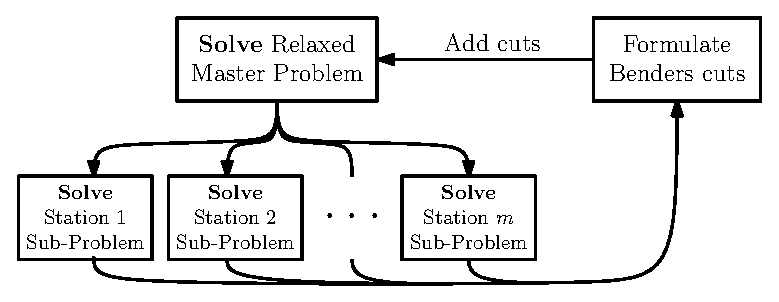
\includegraphics[width=0.9\textwidth]{images/ourHighLevelBenders.eps}
	\label{fig:bend:highLevelBend}
\end{figure}

% \begin{table}[tpb]
% 	\def\arraystretch{1.1}
% 	\centering
% 	\caption{cp vs. mip}
% 	\vspace{2mm}
% 	\begin{tabular}{lp{0.38\textwidth}p{0.38\textwidth}}
% 		\toprule
% 		& CP & MIP \\\midrule
% 		variables & finite domain & binary, integer, continuous \\
% 		constraints & symbolic $(\Rightarrow,\:\cumu,\:\ldots)$ & linear, algebraic $(+,\:*,\:=,\:\leq,\:\ldots)$ \\
% 		inference & propagation & LP relaxation \\
% 		strength & local feasibility & global optimality \\
% 		\bottomrule
% 	\end{tabular}
% 	\label{tab:intro:cpvip}
% \end{table}

% \authciteb{Hooker2003} --- a lot of good motivation for employ logic-based
% Benders.

% \authciteb{Jain2001} \authciteb{Li2009a} --- motivating the use of hybridizing the solution
% methodology.

\section{Types of Sub-Problems}
\label{sec:bend:SPtype}
When using logic-based Benders decomposition, there are two general types 
of sub-problems which can be implemented: optimality sub-problems and 
feasibility sub-problems.
We now detail the unique qualities of each 
type and discuss their possible advantages and disadvantages when 
applied to the \sua{2}.

\subsection{Feasibility Sub-Problems}
\label{sec:bend:SPfeas}
Using feasibility sub-problems means that we are only required to check if 
the relaxed master's current solution is feasible.
If the sub-problems are found to be infeasible given the master's cycle time, 
then a cut-set is sent back to the master to remove
this assignment and similar assignments from the master's feasible solution space.
Testing for infeasibility can be a fast procedure as only
one sub-problem needs to report that its assignment cannot
satisfy the master's cycle time.
Although the trade-off here is that feasibility sub-problems
provide a comparatively small amount of information when compared to optimality sub-problems.
This could mean that the speed we gain from only testing for
feasibility could be dwarfed by the reduction in cut quality.
In fact, low quality Benders cuts can lead to more iterations of
the algorithm being required; if the primary bottleneck in computational runtime
is due to the master then simpler sub-problems may not
provide an overall runtime reduction.
Even so, it is not necessarily the case that feasibility sub-problems 
are strictly worse than optimality sub-problems.

In the case of the \sua{2} we have $m$ sub-problems at 
each iteration of the decomposition. 
If we consider feasibility sub-problems, then there are two simple 
but quite distinct ways which the cutting procedure could 
possibly be formulated. 
% We detail these here and what is gained and lost with each formulation.
\begin{itemize}
	\item \emph{Solve all sub-problems}. By testing the feasibility of each station's
	assignment, we find out all stations which are infeasible
	and all which can satisfy the cycle time.
	This allows $k$ Benders cuts to be made where $k$ is the number
	of sub-problems where infeasibility is detected ($k \leq m$).
	Each sub-problem can be run in parallel which can vastly reduce the solution
	time of the sub-problems, however parallel computation isn't strictly necessary
	in this case.
	\item \emph{Solve until infeasibility}. Run all sub-problems in parallel until
	one detects infeasibility, then terminate all other problems.
	This procedure will be much faster than the last however we gain far less information
	from the sub-problems.
	In this case we can make only two Benders cuts.
	The sub-problem which found infeasibility results in a Benders cut
	that removes its assignment of tasks from the master's feasible region.
	We can also make a weaker cut that removes the
	full assignment of tasks from occurring in future
	iterations.
\end{itemize} 

In both cases of feasibility sub-problems, the information
gained is limited and so the range of Benders cuts we can formulate
is quite restricted.
The feasibility cuts we considered are presented later in Section \ref{sec:bend:NGcuts}.

\subsection{Optimality Sub-Problems}
\label{sec:bend:SPopt}
Programming the scheduling problem within each
station as an optimality sub-problem means that
the optimal sequence of tasks within each station
will be found; irrelevant of whether a station's
load can respect the master's cycle time estimate.
The disadvantage of this when compared to
just testing for infeasibility, is that
solving each combinatorial scheduling problem
to optimality may be far more time consuming.
The primary advantage is that at each iteration
of the Benders algorithm, we receive richer information
from the sub-problems allowing more flexibility in
the Benders cuts we devise.

% Unlike feasibility sub-problems, there is little computational speed we can gain
% by taking advantage of parallel computing here.
% Running all sub-problems in parallel could certainly
% result in a reduction in total runtime, but as each
% scheduling problem needs to be solved to optimality, there is no more
% we can gain via the communication of solutions between sub-problems.

We predominantly explored the use of optimality cuts in our
Benders decomposition and in the coming sections 
(see \ref{sec:bend:Icuts1}--\ref{sec:bend:Logcuts}) we will
provide their formulation.

\section{Relaxed Master Problem}
\label{sec:bend:RMP}
The relaxed master problem handles the assignment
of tasks to stations.
As mixed-integer programming is an effective solving technology for
allocation problems (refer to Section \ref{sec:lit:hybridBend})
we formulated the RMP as a MIP.

Let the current iteration of the Benders
algorithm be indexed by $\mu$
and a previous iteration by $\nu$.
We now present the formulation of the RMP 
at the $\mu^{th}$ iteration, which we will denote
by \rmp{\mu}.
% The decision variables of this program are summarised
% in Table \ref{tab:bend:RMPvars}.
The cycle time variable, $c^\mu$, and the assignment
variables, $x_{ik}^\mu$, have equivalent definitions
as in the previous chapter but are now also indexed by the 
Benders iteration counter.
% Variables $y_{ijk}$ and $z_{ijk}$ allow the master to decide
% upon a sequencing of the tasks within each station
% and these variables are defined equivalently as in the previous
% chapter.
The complications presented by the sequencing problems
are omitted from the RMP and as a result the total setup
cost of each station is taken as zero.
% The estimated setup cost of station $k$ is decided by
% variable $\xi_k$.

% \begin{table}[tbp]
% 	\def\arraystretch{1.1}
% 	\centering
% 	\caption{Decision variables of the Relaxed Master Problem at iteration $\mu$}
% 	\vspace{2mm}
% 	\begin{tabular}{lp{0.8\textwidth}}
% 		\toprule
% 		Variable & Definition \\\midrule
% 		$c^\mu$ & cycle time of the assembly line, continuous\\
% 		$x_{ik}^\mu$ & 1 iff task $i \in V$ is assigned to station $k \in FS_i$ \\
% 		$y_{ijk}$ & 1 iff task $i \in V$ is followed directly by task $j \in F_i^\phi$ in the forward station load of station $k \in FS_i$ \\
% 		$z_{ijk}$ & 1 iff task $i \in V$ is the last task completed and task $j \in F_i^\beta$ is the first in station $k\in FS_i$ \\
% 		$\xi_{k}$ & Lower bound on the total setup time of station $k\in K$, continuous \\ 
% 		\bottomrule
% 	\end{tabular}
% 	\label{tab:bend:RMPvars}
% \end{table}

% \begin{IEEEeqnarray}{rClCl}
% 	\IEEEeqnarraymulticol{3}{l}{\text{\rmp{\mu}: Min } c^\mu} & \hspace{4mm} & \label{eq:bend:rmp1}\\[\eqnv]
% 	\text{s.t. } & \hspace{4mm} & \sum_{k\in FS_i} x_{ik}^\mu = 1 & & \forall i \in V \label{eq:bend:rmp2}\\[\eqnv]
% 	& & \sum_{j\in F_i^\phi} y_{ijk} + \sum_{j\in F_i^\beta}z_{ijk} = x_{ik}^\mu & & \forall i \in V,~ k\in FS_i \label{eq:bend:rmp3}\\[\eqnv]
% 	& & \sum_{i\in P_j^\phi} y_{ijk} + \sum_{i\in P_j^\beta}z_{ijk} = x_{jk}^\mu & & \forall j \in V,~ k\in FS_j \label{eq:bend:rmp4}\\[\eqnv]
% 	& & \sum_{i \in FT_k}\sum_{j\in F_i^\beta} z_{ijk} \geq 1 & & \forall k\in K \label{eq:bend:rmp5}\\[\eqnv]
% 	& & \sum_{k \in FS_i} k\cdot x_{ik}^\mu \leq \sum_{k \in FS_j} k\cdot x_{jk}^\mu & & \forall (i,j) \in E \label{eq:bend:rmp6}\\[\eqnv]
% 	& & \sum_{i \in V} t_i \cdot x_{ik}^\mu + \xi_{k} \leq c^\mu & & \forall k \in K \label{eq:bend:rmp7}\\[\eqnv]
% 	& & \xi_k = \sum_{i \in FT_k} \left( \sum_{j \in F_i^\phi} \phi_{ij}\cdot y_{ijk} + \sum_{j \in F_i^\beta} \beta_{ij}\cdot z_{ijk} \right) & & \forall k \in K \label{eq:bend:rmp8}\\[\eqnv]\
% 	& & C(i) & & i \in \{1, 2,\ldots,\mu-1 \} \label{eq:bend:rmp9}\\[\eqnv]
% 	& & \ul{c}^\mu\leq c^\mu \leq \bar{c}^\mu & &  \label{eq:bend:rmp10}\\[\eqnv]
% 	& & 0 \leq \xi_k \leq \bar{c} & & \forall k \in K \label{eq:bend:rmp11}\\[\eqnv]
% 	& & x_{ik}^\mu\in\{0,1\} & & \forall i \in V,~ k \in FS_i \label{eq:bend:rmp12}\\[\eqnv]
% 	& & y_{ijk}\in\{0,1\} & & \forall i \in V,~ j \in F_i^\phi,~ k \in FS_i \nonumber\\[\smolEqnv]
% 	& & & & \label{eq:bend:rmp13}\\[\eqnv]
% 	& & z_{ijk}\in\{0,1\} & & \forall i \in V,~ j \in F_i^\beta,~ k \in FS_i \nonumber\\[\smolEqnv]
% 	& & & & \label{eq:bend:rmp14}
% \end{IEEEeqnarray}

\begin{IEEEeqnarray}{rClCl}
	\IEEEeqnarraymulticol{3}{l}{\text{\rmp{\mu}: Min } c^\mu} & \hspace{4mm} & \label{eq:bend:rmp1}\\[\eqnv]
	\text{s.t. } & \hspace{4mm} & \sum_{k\in FS_i} x_{ik}^\mu = 1 & & \forall i \in V \label{eq:bend:rmp2}\\[\eqnv]
	& & \sum_{k \in FS_i} k\cdot x_{ik}^\mu \leq \sum_{k \in FS_j} k\cdot x_{jk}^\mu & & \forall (i,j) \in E \label{eq:bend:rmp3}\\[\eqnv]
	& & \sum_{i \in V} t_i \cdot x_{ik}^\mu \leq c^\mu & & \forall k \in K \label{eq:bend:rmp4}\\[\eqnv]
	& & \mathcal{C}^\nu & & \nu \in \{1, 2,\ldots,\mu-1 \} \label{eq:bend:rmp5}\\[\eqnv]
	& & \ul{c}^\mu\leq c^\mu \leq \bar{c}^\mu & &  \label{eq:bend:rmp6}\\[\eqnv]
	& & x_{ik}^\mu\in\{0,1\} & & \forall i \in V,~ k \in FS_i \label{eq:bend:rmp7}
\end{IEEEeqnarray}

The objective is to minimize the cycle time estimate in (\ref{eq:bend:rmp1}).
Constraint (\ref{eq:bend:rmp2}) ensures each task
is assigned exactly one station.
We ensure the precedence relations are satisfied between stations with
constraint (\ref{eq:bend:rmp3}).
Each station's total workload, \ie sum of task processing times,
is required to respect the cycle time through constraint (\ref{eq:bend:rmp4}).
Finally, the set of Benders cuts found in the previous iterations are included
in the master in constraint (\ref{eq:bend:rmp5}).
The remaining constraints define the domains of
each decision variable.

We note here that unlike the MIP formulations presented in the
previous chapter, this relaxed formulation of just the
assignment portion has not required any disjunctive constraints.
Hence, the linear relaxation used throughout the \bab algorithm
of the Gurobi solver will likely be far tighter.

% The RMP is in fact very close to a full formulation
% of the \sua{2}, with only a single requirement removed.
% This is the constraint that within each station we require only a single
% cyclic sequence of tasks.
% So we can view a solution to the RMP as an assignment

\section{Sub-Problems}
\label{sec:bend:SP}
Each of the sub-problems has a similar structure to
the asymmetric Travelling Salesperson Problem
with some forbidden paths.
We can view the tasks as the cities and distance
between any pair of tasks as the setup time.
The asymmetry is due to $\phi_{ij}$ ($\beta_{ij}$) not necessarily
being equal to $\phi_{ji}$ ($\beta_{ji}$).

As the structure of each scheduling problem has a 
highly combinatorial nature we consider 
three approaches:
mixed-integer programming, constraint
programming and fully formulating
the sub-problem as a TSP.
When the sub-problem is formulated
as a constraint program or a TSP,
then the logic-based Benders decomposition
we propose can be seen as a hybrid solution
methodology.

We now define new notation for formulating a
sub-problem.
The set of tasks assigned to station $k$
at iteration $\mu$ is defined as $V_k^\mu \subseteq V$.
The set of precedence relations is given by 
\[
	E_k^\mu = \{\: (i,j) \: | \: i,j \in V_k^\mu\:\} \subseteq E,
\]
The decision variables $y_{ij}$, $z_{ij}$ and $s_{i}$
all have equivalent definitions as in the previous chapter.
The total workload of a station is decided by the variable
$l_k^\mu$.
Table \ref{tab:bend:SPvars} provides a summary of a sub-problem's
decision variables.

\begin{table}[tbp]
	\def\arraystretch{1.1}
	\centering
	\caption{Decision variables of sub-problem $k$ at iteration $\mu$}
	\vspace{2mm}
	\begin{tabular}{lp{0.8\textwidth}}
		\toprule
		Variable & Definition \\\midrule\midrule
		$l_k^\mu$ & Total load of the current station $k$ at iteration $\mu$, $k$ is a parameter for a given sub-problem \\
		$s_i$ & start time of task $i\in V_k^\mu$, continuous \\
		$y_{ij}$ & 1 iff task $i \in V_k^\mu$ is followed directly by task $j \in F_i^\phi$ in the forward station load \\
		$z_{ij}$ & 1 iff task $i \in V_k^\mu$ is the last task completed and task $j \in F_i^\beta$ is the first in the same station \\
		\bottomrule
	\end{tabular}
	\label{tab:bend:SPvars}
\end{table}

\subsection{MIP Sub-Problem Formulation}
\label{sec:bend:mipForm}
Let \spmip{\mu} denote the mixed-integer programming
formulation of the sub-problem at iteration $\mu$.
Given the set $V_k^\mu$ of tasks that need to be sequenced,
we can formulate the MIP as follows

\begin{IEEEeqnarray}{rClCl}
	\IEEEeqnarraymulticol{3}{l}{\text{\spmip{\mu}: Min } l_k^\mu} & \hspace{4mm} & \label{eq:bend:spmip1}\\[\eqnv]
	\text{s.t. } & \hspace{4mm} & \sum_{j \in F_i^\phi} y_{ij} + \sum_{j \in F_i^\beta} z_{ij} = 1 & & \forall i \in V_k^\mu \label{eq:bend:spmip2}\\[\eqnv]
	& & \sum_{i \in P_j^\phi} y_{ij} + \sum_{i \in P_j^\beta} z_{ij} = 1 & & \forall j \in V_k^\mu \label{eq:bend:spmip3}\\[\eqnv]
	& & \sum_{i\in V_k^\mu} \sum_{j\in F_i^\beta} z_{ij} =1 & &  \label{eq:bend:spmip4}\\[\eqnv]
	& & s_i + t_i + \phi_{ij}\cdot y_{ij} \leq s_j & & \forall (i,j) \in E_k^\mu \label{eq:bend:spmip5}\\[\eqnv]
	& & s_i + t_i + \phi_{ij} \leq s_j + M(1-y_{ij}) & & \forall i\in V_k^\mu,~ j \in F_i^\phi  \label{eq:bend:spmip6}\\[\eqnv]
	& & s_i + t_i + \sum_{j\in F_i^\beta}\beta_{ij}\cdot z_{ij} \leq l_k^\mu & & \forall i\in V_k^\mu \label{eq:bend:spmip7}\\[\eqnv]
	& & l_k^\mu \geq 0 & &  \label{eq:bend:spmip8}\\[\eqnv]
	& & s_i \geq 0 & & \forall i \in V_k^\mu \label{eq:bend:spmip9}\\[\eqnv]
	& & y_{ij}^\mu\in\{0,1\} & & \forall i \in V_k^\mu,~ j \in F_i^\phi \label{eq:bend:spmip10}\\[\eqnv]
	& & z_{ij}^\mu\in\{0,1\} & & \forall i \in V_k^\mu,~ j \in F_i^\beta \label{eq:bend:spmip11}
\end{IEEEeqnarray}

Together constraints (\ref{eq:bend:spmip2}) and (\ref{eq:bend:spmip3})
ensure that each task in the station's cyclic sequence
has exactly one successor and one predecessor respectively.
Only one backward setup cost exists in the sequence due
to (\ref{eq:bend:spmip4}) and
the precedence relations are enforced by (\ref{eq:bend:spmip5}).
The disjunctive constraint (\ref{eq:bend:spmip6}) requires
that if tasks $j$ directly follows task $i$ in the sequence,
then the setup cost is observed.
Finally, constraint (\ref{eq:bend:spmip7}) bounds the total station
load below by the completion time of the last task in the station.

Decomposing the full MIP formulation into the assignment and scheduling
components has significantly reduced the number of disjunctive constraints
required. Although, to correctly encode the forward setup time
we still require one disjunctive constraint in \spmip{}.

\subsection{CP Sub-Problem Formulation}
\label{sec:bend:cpForm}
Let \spcp{\mu} denote the CP
formulation of the sub-problem at iteration $\mu$.
We considered a constraint programming formulation
of the sub-problem as CP
is a powerful solution technology available
for scheduling problems (see Section \ref{sec:lit:cp}).

Here we will detail the CP model we formulated
and the various advantages that this approach
provides.
Note, that we will give simplified
snippets of the MiniZinc code of our
CP model.

\subsubsection{Basic CP Model}
\label{sec:bend:cpModel}
The majority of the CP model is very similar
to the MIP.
To give the reader an idea of how a constraint
from a MIP can instead be represented in a constraint program,
we now provide the MiniZinc code which equivalently
encapsulates linear constraint (\ref{eq:bend:spmip2}).
\begin{lstlisting}[language=minizinc]
constraint forall ( i in TASK ) (
      sum( j in followForward[i]  )( y[i,j] )
    + sum( j in followBackward[i] )( z[i,j] ) == 1
);
\end{lstlisting}%\vspace{5mm}
The set {\tt TASK} is equivalent to $V_k^\mu$ in the MIP,
while {\tt followForward[i]} and \newline{\tt followBackward[i]} correspond to
$F_i^\phi$ and $F_i^\beta$ respectively.

All other constraints from the MIP translate in similar ways and
for brevity we will only note the main differences between the
two models.
For the full specification of the CP program, 
we refer the reader to the MiniZinc code included
in the Appendices \ref{lst:appen:CPmodel}.
The expressive nature of CP allows us to more effectively
encode the disjunctive constraint from (\ref{eq:bend:spmip6}).
This can be done as follows,
\begin{lstlisting}[language=minizinc]
constraint forall ( i in TASK, j in followForward[i] ) (
    y[i,j] <-> ( s[i] + dur[i] + forwardSetup[i,j] == s[j] )
);
\end{lstlisting}%\vspace{5mm}
Where {\tt dur[i]} corresponds to $t_i$ and {\tt forwardSetup}
stores the two-dimensional array of forward setup times, $\phi_{ij}$.
Using the bijection operator, {\tt <->}, offered by MiniZinc,
we are able to succinctly create two conditional constraints
in the constraint model.
Also, notice that previously this constraint was encoded
as an inequality, however now we are able to fix the starting
time of task $j$ if we know that task $i$ is its direct predecessor.
The flexibility and expressiveness of the CP language MiniZinc
has allowed us to remove many of the negative qualities of this disjunctive
constraint.

\subsubsection{Global Scheduling Constraints}
\label{sec:bend:cpGlob}
Many scheduling problems have been effectively solved
by CP due to the powerful propagation qualities
of the global constraints.
We will now briefly detail some of the global constraints
that are well-suited to our problem
and how they can be utilized.
Note that the constraints presented here
have been somewhat simplified and some of their
more complex functionality is not regarded.

Since within each station no two tasks can be executed
concurrently, the \newline\disj constraint can model this non-overlap property.
This global constraint takes as input two arrays related to a
task: variable start times, 
and fixed durations.
\begin{lstlisting}[language=minizinc]
disjunctive( array of var int: start,
             array of int: dur );
\end{lstlisting}%\vspace{5mm}
In our problem we have start time variables $s_i$
and fixed processing durations $t_i$ for each task,
which suggests \disj could be suited to a sub-problem.
However, the actual duration between any two tasks
$i$ and $j$ is not just the processing time of task $i$,
but also the setup cost $\phi_{ij}$.
Since this setup cost depends on the task ordering, the
duration cannot be fixed.
As such, \disj may not provide as effective propagation
as another global constraint.

The global constraint \cumu ~--- previously described
in Section \ref{sec:lit:cpGlob} ---
is similar to \disj but requires two further
pieces of input: the quantity of resources that each task
requires and also the limit of total available resources.
\begin{lstlisting}[language=minizinc]
cumulative( array of var int: start, 
            array of int: dur, 
            array of var int: resourceRequirement, 
            int: resourceLimit );
\end{lstlisting}%\vspace{5mm}
In our case only one task can be processed within
a station, so we define the resource limit to be 1.
To overcome the problem encountered with the \disj constraint
we introduce a new set of decision variables that are added to
\spcp{}. For each pair of tasks in $V_k^\mu$ we add the continuous variable $\sigma_{ij}$ defined as follows
\[
	\sigma_{ij} =\displaystyle
	\begin{cases}
	s_i &\text{if } y_{ij}=1,\\
	0 &\text{otherwise}.
	\end{cases}
\]
Now that we have a variable defining the start time
of a task $i$ which also depends on task $i$'s place
in the sequence, we can use the \cumu constraint to more accurately
encode the non-overlapping quality of the tasks.
\begin{lstlisting}[language=minizinc]
constraint cumulative(
    [ sigma[i,j]                 | i in TASK, j in TASK ],
    [ dur[i] + forwardSetup[i,j] | i in TASK, j in TASK ],
    [ y[i,j]                     | i in TASK, j in TASK ],
    1
);
\end{lstlisting}%\vspace{5mm}
The start time variables given to cumulative
are the $\sigma_{ij}$ variables.
This requires the \cumu constraint to handle the scheduling of
$n^2$ variables rather than just $n$.
But we hope that
the intelligent propagation it will provide
will outweigh the cost.
Each $\sigma_{ij}$ variable has only a single
corresponding $\phi_{ij}$ and so the durations
sent to \cumu are now fixed values.
Notably, the resource requirement of each task has been
given to the constraint as the variable $y_{ij}$.
So if task $j$ does not directly follow task $i$ in the
task sequence then $y_{ij}$ will take value 0 and the
resource requirement of the corresponding
task in the \cumu constraint will also be 0, \ie
it will not be considered in the schedule.

By achieving an encoding of the non-overlapping quality
between the tasks of a station using a global constraint,
we have allowed the CP sub-problems to gain access
to the well-studied propagation properties of \cumu.

% \subsubsection{Redundant Constraints}
% \label{sec:bend:cpRedun}
% One of the quirks or the MiniZinc language
% is that no decision variable can be defined
% on a non-contiguous set.
% Although, we need the variables $y_{i,j}$
% to be defined $\forall i\in V$ and $\forall j\in F_i^\phi$.
% However $F_i^\phi$ is not necessarily a 
% contiguous set of tasks and so we
% instead defined the $j$
% index over all tasks, \ie $\forall i\in V,~j\in V$.
% Similarly for the $z_{ij}$ variables and the 
% set $F_i^\beta$.
% Consider the following two constraints:
% \begin{lstlisting}[language=minizinc]
% constraint forall ( i in TASK, j in TASK
%                     where not( j in followForward[i] ) ) (
%     y[i,j] == 0
% );
% constraint forall ( i in TASK, j in TASK
%                     where not( j in followBackward[i] ) ) (
%     z[i,j] == 0
% );
% \end{lstlisting}%\vspace{5mm}
% These constraints fix the values of the 
% decision variables $y_{ij}$
% and $z_{ij}$ whose values are known \ap.
% Including these constraints, reduces the 
% amount for work necessary for the solver.

\subsubsection{Search Procedure}
\label{sec:bend:cpSearch}
MiniZinc provides a search language containing
a range of basic search procedures, 
such as \intser and \bolser,
as well as a compositional search procedure,
\seqser, which allows the user to define
problem-specific search strategies.
This allows the user utilize their
familiarity with the problem to direct the 
search tree of the CP solver toward areas
which will likely provide good feasible
solutions.
We note here that including the auxiliary 
variable $\sigma_{ij}$ in the CP model
allowed us to formulate a wider range of
potential search strategies.

We considered a range of basic and compositional
search procedures.
A simplified representation of
the basic procedures are as follows
\begin{lstlisting}[language=minizinc]
ann: start_io = int_search( s, input_order,      indomain_min );
ann: start_sm = int_search( s, smallest,         indomain_min );
ann: start_sl = int_search( s, smallest_largest, indomain_min );  
ann: start_ff = int_search( s, first_fail,       indomain_min ); 

ann: sigma_ff = int_search( [ sigma[i,j] | i in TASK, j in TASK ],
                                first_fail, indomain_max );
\end{lstlisting}%\vspace{5mm}

To briefly illustrate how these procedures
operate, we consider the {\tt start\_sm} search.
In this case, the CP solver will choose to branch on the
start time variables of the tasks first.
The first start time variable that will be chosen, say $s_i$,
will be the one with the smallest value in its domain;
governed by the {\tt smallest} variable selection.
Once chosen, two new nodes will be created:
one with the value of $s_i$ fixed to its smallest
value, and one where this smallest value is removed from
$s_i$'s domain.

We compose these five search annotations in a number of ways using
the \newline{\tt seq\_search} procedure as follows
\begin{lstlisting}[language=minizinc]
ann: start_io_Then_sigma = seq_search([ start_io, sigma_ff ]);
ann: start_sm_Then_sigma = seq_search([ start_sm, sigma_ff ]);
ann: start_sl_Then_sigma = seq_search([ start_sl, sigma_ff ]);
ann: start_ff_Then_sigma = seq_search([ start_ff, sigma_ff ]);
\end{lstlisting}%\vspace{5mm}
Take for example, {\tt start\_sm\_Then\_sigma}.
In this case the start time variables $s_i$ are fully decided
before moving to the $\sigma_{ij}$ variables.
Although having a full solution to $s_i$ will necessarily 
fix all values the $\sigma_{ij}$ variables, since
the full sequence of tasks has been found.
Hence, the compositional procedure has in fact provided
little benefit for us here.

In our computational experiments we compare the
results of some of these basic and compositional
procedures.
Further to this, we compare these results
against the default search of the CP solver
\chuffed to check whether guiding the
branching of the search tree provides a benefit
for this problem.

\subsubsection{Priority Search}
\label{sec:bend:cpPriSearch}
A recent advancement to the search
functionality of MiniZinc by \authciteb{Young2017b}
has provided a new search combinator:
\priser.
We give a brief summary of this compositional
procedure and detail how we have used it
to formulate new search strategies.

The \priser procedure is defined as
\begin{lstlisting}[language=minizinc]
ann: priority_search( ann, ann, array[int] of ann )
\end{lstlisting}%\vspace{5mm}
where the first and second input annotations
can be defined as \emph{selvars} (selection variables)
and \emph{varsel} (selection criteria).
Similar to the sequential search combinator, this search
takes as input an array of other search procedures.
However the extra functionality that \priser
offers is the ability to dynamically change how
the array of search annotation inputs are ordered.
This is unlike the \seqser procedure which required
a fixed list that could not be changed as the search
progressed.
\priser offers the user more flexibility than was previously
available due to the ability to nest priority search strategies.

Here we provide one example of a \priser
that we considered and detail how three other similar
priority search strategies can be formulated.
\begin{lstlisting}[caption={Priority search used for CP sub-problems},label={lst:bend:priser},language=minizinc]
ann: priority_ff = priority_search( s, first_fail,
    [seq_search([
                int_search([ s[i] ],                   first_fail, indomain_min)
                int_search([ sigma[i,j] | j in TASK ], first_fail, indomain_min) ])
    | i in TASK ]
);
\end{lstlisting}\vspace{5mm}
This search is also formulated in three similar ways by
using the {\tt input\_order}, {\tt smallest} and {\tt smallest\_largest}
variable selection strategies instead of {\tt first\_fail}.

As noted earlier, the compositional search
procedure we considered gained little upon the basic
searches they combined.
The priority search, given in Listing \ref{lst:bend:priser},
branches first on the start time of the task
with the fewest possible values in its domain, say task $i$. 
% because of variable selection strategy {\tt first\_fail}.
Once $s_i$ is fixed, we then search over the
start times of variables that can follow task $i$,
\ie the variables $\sigma_{ij}$.
Priority Search allows us to quickly remove
possible followers from consideration and guide the
branching of the search procedure.


\subsection{TSP Sub-Problem Formulation}
\label{sec:bend:TSP}
Let \sptsp{\mu} denote the TSP
formulation of the sub-problem at iteration $\mu$.
Since the sequencing problem within each station is similar to the 
asymmetric version of the TSP, we assumed that
employing a dedicated TSP solver, such as Concorde \cite{Applegate2017},
would be a desirable approach to the sub-problems.

The TSP solver Concorde has been shown to be exceptionally
effective at tackling the symmetric case of the TSP;
solving instances of up to 85,900 cities.
Although the input to the solver is restricted to just 
the symmetric version, if we are able to represent a
station's sub-problem as a symmetric TSP then the computational
runtime reduction may be worthwhile.

Converting an asymmetric TSP to a symmetric version is a straightforward
procedure that results in the number of cities being doubled.
So overcoming that obstacle is possible, however the differentiation
between forward and backward setup times poses another
problem.
This difference means that the city where the travelling salesperson
begins and the final city they visit has an impact on the total tour
length (due to the backward setup).
This complication results in a sub-problem
being distinctly different (but closely related) 
to the TSP.
This difference proved difficult to overcome early in our
exploration of this formulation.
As a result, we focused our attention on the other
possible sub-problems and did not pursue
a TSP formulation further.
However, we do encourage the enthusiastic reader to try their hand 
at such a formulation.

\section{Cuts}
\label{sec:bend:cuts}
The quality of the Benders cuts formulated from the solution
of the sub-problems directly impact the
speed with which the Benders decomposition will
approach the optimal solution.
As such, we considered a range of cuts which
can be added to the master problem, after
all sub-problems have been resolved.
% One type of feasibility cut was devised and is presented in
% Section \ref{sec:bend:NGcuts}.
% The remaining cuts are all instances of optimality
% cuts and are given in Sections \ref{sec:bend:Icuts1}--\ref{sec:bend:Logcuts}.

For this section we introduce new notation detailed
in Table \ref{tab:bend:notationProofs}.
Using this notation we represent a solution to the master 
by its assignment and cycle time
variables as $S^{\nu}=\{[x_{ik}^\nu],c^\nu\}$,
and the optimal solution is represented as
$S^{\nu*}=\{[x_{ik}^{\nu*}],c^{\nu*}\}$.
\begin{table}[tbp]
	\def\arraystretch{1.1}
	\centering
	\caption{Notation for proofs}
	\vspace{2mm}
	\begin{tabular}{lp{0.8\textwidth}}
		\toprule
		Notation & Definition  \\\midrule\midrule
		$\mathcal{C}^\nu$ & The set of all cuts added to the RMP at iteration $\nu$ of the Benders algorithm\\
		$\mathcal{C}_x^\nu$ & The set of type-$x$ cuts added to the RMP at iteration $\nu$, where \newline $x\in\{\:ng,\:i,\:ii,\:iii,\:ub,\:l\:\}$, \eg $\mathcal{C}_{ng}^\nu$ denotes the set of nogood cuts\\
		$\mathcal{F}^\nu$ & The feasible solution space of \rmp{\nu}\\
		$S^\nu ~(S^{\nu*})$ & A feasible (optimal) solution to \rmp{\nu}, $S^\nu\in \mathcal{F}^\nu$\\
		$[x_{ik}^\nu]~ \big( [x_{ik}^{\nu*}] \big)$ & A feasible (optimal) solution to the assignment decisions of \rmp{\nu} \\
		\bottomrule
	\end{tabular}
	\label{tab:bend:notationProofs}
\end{table}

\subsection{Nogood Cut}
\label{sec:bend:NGcuts}
A \emph{nogood} is a partial solution to a problem which prevents
a full feasible solution from being obtained.
In our case, we considered a partial solution to the full problem
to be an assignment of tasks to a single station.
If we consider sub-problem $k$ at iteration $\nu$
then when $l_k^\nu \not\leq c^\nu$ a nogood cut
can be added to the master problem to remove this
partial solution from the feasible solution
space of \rmp{\mu}, where $\mu=\nu+1,\:\nu+2,\:\ldots$.

We now present the formulation of the nogood cut
added to the \rmp{} at iteration $\nu$
and considered for all iterations $\mu>\nu$.
\begin{IEEEeqnarray}{rCcCl}
	\mathcal{C}_{ng}^\nu:&\hspace{4mm}& c^\nu+1-\sum_{k\in K}\sum_{i\in V_k^\nu}(1 - x_{ik}^\mu) \leq c^\mu. &\hspace{4mm}& \label{eq:bend:ngcut}
\end{IEEEeqnarray}
For this to be a valid cut, we require that the current solution,
$S^{\nu*}$, is no longer possible in all
future master problems, \ie
\[ S^{\nu*}\not\in\mathcal{F^\mu},~\forall \mu\in\{\:\nu+1,\:\nu+2,\ldots\:\}, \]
and also that the cut does not remove any globally optimal
solutions.
As we only add the cut when a sub-problem cannot respect the
master's tentative cycle time value, no globally optimal
solutions can be removed.

\begin{theorem}\label{thm:bend:ngcut}
	The proposed nogood cut (\ref{eq:bend:ngcut}) is valid.
\end{theorem}
\begin{proof}
	There are two cases to consider: the solution to the \rmp{\mu}
	has the same task assignment and a different task assignment to
	\rmp{\nu}.
	\begin{itemize}
		\item[a)] $[x_{ik}^{\nu*}] = [x_{ik}^{\mu*}]$ .	
		In this case the nogood cut (\ref{eq:bend:ngcut}) reduces to
		\[ c^\nu +1 \leq c^\mu ~\Rightarrow ~c^\nu < c^\mu. \]
		Thus, when the assignment is equivalent, the cycle times
		must be different.
		\item[b)] $[x_{ik}^{\nu*}] \neq [x_{ik}^{\mu*}]$.
		Adding $\mathcal{C}_{ng}^\nu$ removed at least $S^{\nu*}$
		from the feasible solution space of \rmp{\mu}.
	\end{itemize}
	In case a), the solution differs by cycle time value and 
	in case b), the solution differs by task assignment, so
	$S^{\nu*}\not\in\mathcal{F^\mu}$.
	Hence, (\ref{eq:bend:ngcut}) is a valid cut.
\end{proof}

To show that the Benders decomposition algorithm
will find the global optimal solution, 
we require Lemma \ref{lem:bend:bendFinite}.

\begin{lemma}\label{lem:bend:bendFinite}
	The Benders decomposition algorithm
	terminates in a finite number of 
	iterations when adding a valid cut
	at each iteration.
\end{lemma}
\begin{proof}
	After iteration $\mu$ of the algorithm, either all sub-problems
	can satisfy the current cycle time,
	or at least one station cannot satisfy $c^\mu$.
	Cases:
	\begin{itemize}
		\item[a)] $\forall k\in K$  $l_k^\mu\leq c^\mu$.
		The solution to \rmp{\mu} is optimal and we terminate.
		\item[b)] $\exists k\in K$ such that $l_k^\mu\not\leq c^\mu$.
		Add the corresponding cut to all future RMPs.
	\end{itemize}
	In case b), since the cut added is valid,
	at least one feasible solution 
	is removed from the master problem.
	We also know that the \rmp{} has a finite number of feasible integer solutions.
	Hence, the Benders decomposition algorithm will terminate
	in a finite number of iterations.
\end{proof}

\subsection{First Infer Cut}
\label{sec:bend:Icuts1}
The \emph{infer} cuts we devised are examples
of optimality cuts, where each sequencing sub-problem
is solved to optimality at each iteration of the
Benders algorithm.
By comparing the current optimal solution of the \rmp{}
to the optimal solution of a station, we can make 
an inference about the set of tasks assigned this station.
The first kind of inference we make is the simplest
of those we considered and can be described as follows.

At iteration $\nu$ after all sub-problems have been solved
to optimality, assume that $\exists k\in K$ such that
$l_k^\nu>c^\nu$, \ie
station $k$'s  optimal sequence of tasks cannot respect
the master's cycle time.
At a later iteration, $\mu$, if we have the same assignment
of tasks to station $k$,
then we can infer that the master's cycle time must be at least the
optimal load of station $k$ found previously at iteration $\nu$, $l_k^\nu$.
This inference can be formulated as the following implication:
\[ \big([x_{ik}^{\nu*}] = [x_{ik}^{\mu*}]\big)~\Rightarrow~(l_k^\nu\leq c^\mu). \]
We can model this implication as a disjunctive constraint in the \rmp{}.
The infer cut found at iteration $\nu$ for a given station $k$
and added to \rmp{\mu} where $\mu>\nu$, is formulated
as follows,
\begin{IEEEeqnarray}{rCcCl}
	\mathcal{C}_{i}^\nu:&\hspace{4mm}& l_k^\nu -M \sum_{i\in V_k^\nu} (1-x_{ik}^\mu) \leq c^\mu. &\hspace{4mm}& \label{eq:bend:icuts1}
\end{IEEEeqnarray}
We note that to capture this disjunction in the \rmp{}, a big-$M$ value 
was required.
As the master problem is solved using a MIP solver,
this cut could have undesirable effects on the
linear relaxation.

We now prove that the infer cut (\ref{eq:bend:icuts1}) is valid.
The proof proceeds similarly to the proof of the nogood cut above.

\begin{theorem}
	The proposed infer cut (\ref{eq:bend:icuts1}) is valid.
\end{theorem}
\begin{proof}
	Let $k$ be the station which caused the infer cut to
	be added in iteration $\nu$, \ie $l_k^\nu>c^\nu$.
	There are two cases to consider: when \rmp{\mu} has the 
	same task assignment and a different task assignment to \rmp{\nu}.
	\begin{itemize}
		\item[a)] $[x_{ik}^{\nu*}] = [x_{ik}^{\mu*}]$.
		The infer cut (\ref{eq:bend:icuts1}) reduces to
		\[ l_k^\nu \leq c^\mu. \]
		In this case we know the optimal possible sequencing
		of the tasks assigned station $k$.
		Thus we receive a lower bound on
		$c^\mu$ which must respect $l_k^\nu$.
		The infer cut was added due to $c^\nu<l_k^\nu$
		so we know that $c^\nu\neq c^\mu$ in this case.
		\item[b)] $[x_{ik}^{\nu*}] \neq [x_{ik}^{\mu*}]$.
		The assignment to station $k$ is different so we can
		make no inference in this case.
	\end{itemize}
	In both cases $S^{\nu*}$ is not the optimal
	solution to \rmp{\mu}.
	Hence, $S^{\nu*}\not\in F^\mu$ and the cut (\ref{eq:bend:icuts1}) is valid.
\end{proof}

\subsection{Second Infer Cut}
\label{sec:bend:Icuts2}
This inference cut is similar to the last
as we again compare the optimal load values
of each station against the current master's cycle time.
Any station loads which exceed the current cycle time value
cause a cut to be generated.
For this infer cut, further reasoning is made about
the tasks assigned to a given station, which remove
the need of a big-$M$ value.

We introduce the concept of the total \emph{burden}
on the station's workload that a given task contributes.
Let $B_{ik}^\nu$ denote an upper bound of the total burden on station $k$'s workload,
resulting from assigning task $i\in V$ to $k$ in iteration $\nu$.
The burden of a task is a total of its processing time
and all setup costs which it creates in the task
sequence.
To get an upper bound on the burden incurred from
assigning task $i$ to station $k$ at iteration $\nu$,
we need to calculate the following two values:
1) an upper bound on the setup time of task $i$
in the task sequence of $k$ (denoted $\Gamma_{ik}^\nu$) and
2) a lower bound on the setup time that
would occur between the tasks of station $k$ if task $i$ was not assigned 
to $k$ at iteration $\nu$ (denoted $\gamma_{ik}^\nu$).
The burden of a task is calculated by
\[ B_{ik}^\nu = t_i + \Gamma_{ik}^\nu - \gamma_{ik}^\nu, \]
where the upper and lower bounds on
the setup times are calculated as follows
\begin{IEEEeqnarray}{rCCl}
	\Gamma_{ik}^\nu &=& & \max\Big\{\: \big\{\: \phi_{ji} \:|\: j \in P_i^\phi \:\big\}\:\cup \: \big\{\: \beta_{ji} \:|\: j \in P_i^\beta \:\big\}\:\Big\} \nonumber\\[0pt]
	& & + & \max\Big\{\: \big\{\: \phi_{ij} \:|\: j \in F_i^\phi \:\big\}\:\cup \: \big\{\: \beta_{ij} \:|\: j \in F_i^\beta \:\big\}\:\Big\} \label{eq:bend:maxSU}\\[\eqnv]
	\gamma_{ik}^\nu &=& \IEEEeqnarraymulticol{2}{l}{\min\Big\{\: \big\{\: \phi_{i'j} \:|\: j \in F_{i'}^\phi \:\big\}\:\cup \: \big\{\: \beta_{i'j} \:|\: j \in F_{i'}^\beta \:\big\}\: \Big|\: i'\in V_k^\nu\setminus \{i\}\Big\}. }\label{eq:bend:minSU}
\end{IEEEeqnarray}
To account for both setup costs which task $i$ contributes to, the upper bound, $\Gamma_{ik}^\nu$, is the
sum of the setup time occurring directly before task $i$'s execution and the setup
time directly after.
As for the lower bound $\gamma_{ik}^\nu$, if we consider removing
task $i$ from the task sequence of station $k$, then
only one setup cost is needed to ensure the task
sequence remains unbroken.

Using this upper bound on the burden incurred from task $i$
we can formulate the following infer cut
\begin{IEEEeqnarray}{rCcCl}
	\mathcal{C}_{ii}^\nu:&\hspace{4mm}& l_k^\nu -\sum_{i\in V_k^\nu} B_{ik}^\nu(1-x_{ik}^\mu) \leq c^\mu. &\hspace{4mm}& \label{eq:bend:icuts2}
\end{IEEEeqnarray}
We can interpret this as follows.
Suppose that a cut of the form (\ref{eq:bend:icuts2}) was
added after iteration $\nu$ due to the load of station
$k$ begin greater than $c^\nu$.
Later in iteration $\mu$, for each task $i\in V_k^\nu\setminus V_k^\mu$
we subtract an upper bound on the total burden, $B_{ik}^\nu$, incurred
from assigning $i$ to $k$.
So for each task no longer assigned
to station $k$, the bound on the cycle time $c^\mu$
is relaxed.

We prove the correctness of this upper bound on the burden
in Lemma \ref{lem:bend:burdenUB}.
We note here that the insight of this proof
has been adapted from work by \authciteb{Tran2012}.

\begin{lemma}\label{lem:bend:burdenUB}
	$B_{ik}^\nu$ is a true upper bound on the burden incurred from 
	assigning task $i$ to station $k$ in iteration $\nu$.
\end{lemma}
\begin{proof}
	To show that this lower bound on $c^\mu$, where $\mu>\nu$, does not
	remove any globally optimal solution from $\mathcal{F}^\mu$,
	we prove that $B_{ik}^\nu$ is a true
	upper bound on the contribution of a task
	to an optimal schedule.
	We proceed by contradiction, assuming there
	is a schedule that violates the lower bound on the cycle time.

	Given a set of tasks $V_k^\nu$ assigned to
	station $k$ in the current iteration,
	let $l_k^\nu$ be the optimal station
	workload.
	Define two disjoint subsets given by $\bar{V}_k^\mu \cup \hat{V}_k^\mu= V_k^\nu$.
	Assume that in a subsequent iteration $\mu$,
	the set of tasks $\bar{V}_k^\mu$ are assigned station
	$k$.
	The minimal workload for station $k$ is now $\bar{l}_k^\mu$.
	Thus, contrary to our theorem, we have that
	\begin{IEEEeqnarray}{c}
		\bar{l}_k^\mu < l_k^\nu - \sum_{j\in \hat{V}_k^\nu} B_{ik}^\nu. \label{eq:bend:burdenContrad}
	\end{IEEEeqnarray}

	Let $Seq(\bar{V}_k^\mu)$ denote the sequence of tasks in station $k$ corresponding
	to $\bar{V}_k^\mu$.
	It is possible to construct
	a sequence containing all tasks of $V_k^\nu$
	by placing all tasks in $\hat{V}_k^\mu$, one-by-one
	into $Seq(\bar{V}_k^\mu)$.

	Let $\sigma_i$ be the setup time required
	to insert tasks $i\in \hat{V}_k^\mu$ into $Seq(\bar{V}_k^\mu)$.
	We know the station load of this constructed schedule
	to be
	\[ \bar{l}_k^\mu + \sum_{i\in \hat{V}_k^\mu} t_i + \sigma_i. \]

	This is a sequence of all tasks $i\in V_k^\nu$ and must have 
	a total workload greater than or equal to $l_k^\nu$.
	However, $t_i+\sigma_i \leq B_{ik}^\nu$, so we know the following
	is true
	\[  \sum_{i\in \hat{V}_k^\mu} t_i + \sigma_i \leq  \sum_{i\in \hat{V}_k^\mu} B_{ik}^\nu \]

	Thus we receive
	\[ l_k^\nu \leq \bar{l}_k^\nu + \sum_{j\in \hat{V}_k^\mu} B_{ik}^\nu \]
	which contradicts inequality (\ref{eq:bend:burdenContrad}).
	Hence, $B_{ik}^\nu$ is a true upper bound.
\end{proof}

We now prove the validity of this infer cut; again
the proof splits into two cases.

\begin{theorem}
	The proposed infer cut (\ref{eq:bend:icuts2}) is valid.
\end{theorem}
\begin{proof}
	Let $k$ be the station that caused the cut (\ref{eq:bend:icuts2})
	to be added to the \rmp{} after iteration $\nu$.
	There are two cases to consider: when \rmp{\mu} and \rmp{\nu} have the 
	same task assignment and a different task assignment to station $k$.
	\begin{itemize}
		\item[a)] $\forall i \in V ~ x_{ik}^{\nu} = x_{ik}^{\mu}$.
		The infer cut (\ref{eq:bend:icuts2}) reduces to
		\[ l_k^\nu \leq c^\mu. \]
		In this case we know the optimal possible sequencing
		of the tasks assigned station $k$.
		Thus we receive a lower bound on
		$c^\mu$ which must respect $l_k^\nu$.
		The infer cut was added due to $c^\nu<l_k^\nu$
		so we know that $c^\nu\neq c^\mu$ in this case.
		\item[b)] $\exists i \in V$ such that $x_{ik}^{\nu} \neq x_{ik}^{\mu}$.
		The bound we infer on the cycle time $c^\mu$ is relaxed by 
		$B_{ik}^\nu$.
		From Lemma \ref{lem:bend:burdenUB}, we know that $B_{ik}^\nu$
		is a true upper bound on the burden
		of task $i$.
		Thus, this bound does not remove any globally optimal solution
		from $\mathcal{F}^\mu$.
	\end{itemize}
	In the first case the cycle time must be different
	while in the second the assignment is different, so
	$S^{\nu*}\not\in \mathcal{F}^\mu$.
	Hence, the cut (\ref{eq:bend:icuts2}) is valid.
\end{proof}

\subsection{Third Infer Cut}
\label{sec:bend:Icuts3}
The final type of inference cut we explored is again
similar to the previous two.
The second infer cut took into account the
effect of removing a task from a station's
task sequence.
Whereas this Benders cut reasons about the effect of inserting
an additional task into the task sequence of a station.

When considering adding a task to a station's
task sequence, we again aim to quantify the total
workload burden that this additional task brings.
However, to get a correct lower bound on the cycle time,
we instead seek a lower bound on the burden incurred
from an additional task.
Let $b_{ik}^\nu$ denote a lower bound on the burden
incurred from assigning task $i\in V\setminus V_k^\nu$ to station $k$
in iteration $\nu$.
Note that the burden of an additional task
is only defined for tasks not already assigned to station $k$.
The lower bound on the burden is defined as follows,
\begin{IEEEeqnarray}{c}
	b_{ik}^\nu = t_i + \bar{\gamma}_{ik}^\nu \nonumber
\end{IEEEeqnarray}
The lower bound on the setup time is calculated slightly differently
here compared to equation (\ref{eq:bend:minSU}); this altered calculation is as follows
\begin{IEEEeqnarray}{rCCl}
	\bar{\gamma}_{ik}^\nu &=& & \min\Big\{\: \big\{\: \phi_{ji} \:|\: j \in P_i^\phi \:\big\}\:\cup \: \big\{\: \beta_{ji} \:|\: j \in P_i^\beta \:\big\}\:\Big\} \nonumber\\[0pt]
	& & + & \min\Big\{\: \big\{\: \phi_{ij} \:|\: j \in F_i^\phi \:\big\}\:\cup \: \big\{\: \beta_{ij} \:|\: j \in F_i^\beta \:\big\}\:\Big\}. \label{eq:bend:icut3minSU}
\end{IEEEeqnarray}
This alteration is due to the fact that when inserting
a new task into a station's task sequence, the newly
inserted task becomes part of two setup costs.
We must take the minimum of both.

Further to this alteration, the upper bound on the burden
of a task being removed from a station's task sequence
is changed.
We now have the following
\begin{IEEEeqnarray}{c}
	\bar{B}_{ik}^\nu = t_i + \Gamma_{ik}^\nu. \nonumber
\end{IEEEeqnarray}
For this infer cut, we no longer take into account the setup cost
required to ensure the task sequence remains unbroken.
Note, this will result is a strictly weaker lower bound being inferred on
the cycle time, as $\bar{B}_{ik}^\nu$ is strictly weaker than $B_{ik}^\nu$.
% Note that taking this setup into account will only increase the
% tightness of the lower bound we can infer on the cycle time, 
% so by not considering it our lower bound is strictly looser.
% The reasoning behind not taking this into account is that 

Our final inference cut is formulated as follows
\begin{IEEEeqnarray}{rCcCl}
	\mathcal{C}_{iii}^\nu:&\hspace{4mm}& l_k^\nu -\sum_{i\in V_k^\nu} \bar{B}_{ik}^\nu(1-x_{ik}^\mu) + \sum_{i\in V\setminus V_k^\nu} b_{ik}^\nu \cdot x_{ik}^\mu \leq c^\mu. &\hspace{4mm}& \label{eq:bend:icuts3}
\end{IEEEeqnarray}

Given that $\bar{B}_{ik}^\nu$ is a weaker upper bound than $B_{ik}^\nu$, 
it must be a true upper bound.
The proof that $b_{ik}^\nu$ is a true lower bound is roughly equivalent to
the proof of Lemma \ref{lem:bend:burdenUB} and is omitted.
We now provide a sketch of the proof for this cut's validity,
due to it being similar to the previous proofs.

\begin{theorem}
	The proposed infer cut (\ref{eq:bend:icuts3}) is valid.
\end{theorem}
\begin{proof}
	Let $k$ be the station that caused the cut (\ref{eq:bend:icuts3})
	to be added to the \rmp{} after iteration $\nu$.

	Similar to the second inference cut,
	the proof separates into two cases: one
	where in some subsequent iteration $\mu$,
	station $k$ has the same assignment and one
	where it differs by at least one task.
	Along the same lines as before, the former case
	results in a new cycle time value, while
	the latter case results in a new assignment.

	So in both cases we have that
	$S^{\nu*}\not\in \mathcal{F}^\mu$.
	Hence, the cut (\ref{eq:bend:icuts3}) is valid.
\end{proof}

\subsection{Global Bound}
\label{sec:bend:GBcuts}
We now devise a global upper bound on the cycle time of 
the problem.
Given that it is generated in a similar way to
the cuts and also allows us to devise
a logic cut in the following section, we include its explanation here.
As with the inference cuts,
this bound requires the optimal solution
of all sub-problems to be found.

After all sub-problems of iteration $\nu$
have been solved to optimality we can compare
the values of $l_k^\nu,~ \forall k\in K$.
Suppose that at least one station's optimal task
sequence cannot satisfy the
cycle time of \rmp{\nu}.
Although the master's tentative cycle time cannot be
respected, the full assignment $[x_{ik}^\nu]$
together with each feasible task sequence found by the sub-problems
constructs a globally feasible solution to the \sua{2}.
We can calculate the cycle time of this feasible solution
in the usual way by taking the maximum load among all
stations.
The cycle time value of this feasible solution
gives us a global upper bound on the cycle time
of any future solution.

We can formulate this global bound found at iteration $\nu$, and applicable
to any subsequent iteration $\mu>\nu$, as follows
\begin{IEEEeqnarray}{rCcCl}
	\mathcal{C}_{ub}^\nu:&\hspace{4mm}& c^\mu \leq \max\{\: l_k^\nu \:|\: k \in K \: \}. &\hspace{4mm}& \label{eq:bend:gbcut}
\end{IEEEeqnarray}
This upper bound is calculated
using the objective value of a globally feasible
solution, and thus must be a true upper
bound on the cycle time of \sua{2}.

This bound can not only be added to all future
master problems, but also to any sub-problem
as an upper bound on the station's total workload.
Notably, this may lead to a sub-problem returning
infeasibility if the optimal task sequence
cannot respect this global bound.
This slightly complicates how we can generate Benders
cuts so we provide some brief reasoning about this now.

Let $\Omega^\nu$ denote the current best upper bound on
the cycle time found using (\ref{eq:bend:gbcut}) at iteration $\nu$.
When constraining sub-problem $k$'s objective value
by this global bound at iteration $\mu$,
there are three possible cases:
\begin{enumerate}
	\item $l_k^\mu \not\leq \Omega^\nu$. The sub-problem
	cannot respect the upper bound and infeasibility is returned.
	In this case, we are only able to generate feasibility cuts.
	\item $c^\mu < l_k^\mu \leq \Omega^\nu$. The station's load can respect
	the upper bound but not the current master's solution.
	Here we can generate optimality cuts as the sub-problem's optimal
	solution is known.
	\item $l_k^\mu \leq c_\mu$. The sub-problem satisfies the current
	master's cycle time and so no cuts are generated.
\end{enumerate}
In the following section we devise a new type of feasibility
cut which can take advantage of the new information that
this global upper bound provides.

\subsection{Logic Cut}
\label{sec:bend:Logcuts}
Generally, a \emph{logic} cut employs reasoning
to remove a set of similar solutions
from the feasible solution space of the relaxed master.
Any infer cut could also be classified as a logic cut,
however the Benders cut we present in this section
is not formulated as an inference.
As such we label it with a more general classification.

The global bound devised in the previous section
resulted in sub-problems possibly
returning infeasibility.
We can use this information to generate a feasibility cut
and add that back to the subsequent master problems.
The nogood cuts we devised earlier could be used in this case,
although we are able to reason further about the information
this global bound provides and
in turn receive a more powerful feasibility cut; 
which we call a logic cut.

Given an upper bound $\Omega^\nu$ on the cycle time generated
by (\ref{eq:bend:gbcut}) in iteration $\nu$, suppose that
at a later iteration $\mu$ we constrain the load
of all sub-problems by this bound.
Now suppose that the station load of sub-problem $k$ 
cannot respect this bound, so we have $l_k^\mu \not\leq \Omega^\nu$.
Since this is a globally feasible upper bound on the cycle time,
we know that the set of tasks assigned to station $k$, $V_k^\mu$,
necessarily leads to infeasibility.
Thus, we can generate an infeasibility cut in the master problem
which removes this assignment from all future solutions.

Given a global upper bound found by (\ref{eq:bend:gbcut})
we formulate a logic cut, as follows
\begin{IEEEeqnarray}{rCcCl}
	\mathcal{C}_{l}^\nu:&\hspace{4mm}& \sum_{i\in V_k^\nu} (1-x_{ik}^\mu) \geq 1. &\hspace{4mm}& \label{eq:bend:logcut}
\end{IEEEeqnarray}
This constraint ensures that at a later iteration $\mu$, the
assignment to station $k$ differs by at least one task from 
$V_k^\nu$.

We now prove the validity of this logic cut.

\begin{theorem}
	The proposed logic cut (\ref{eq:bend:logcut}) is valid.
\end{theorem}
\begin{proof}
	Suppose that at iteration $\nu$, a cut of the form (\ref{eq:bend:logcut})
	was added due to sub-problem $k$ being unable to satisfy the
	current best global upper bound, denoted by $\Omega$.
	Now consider the \rmp{} at a later iteration $\mu$.

	Once more, there are two cases to consider:
	the assignment solution to station $k$ of \rmp{\mu}
	is equivalent to that of \rmp{\nu} and different.
	\begin{itemize}
		\item[a)] $V_k^\nu = V_k^\mu$.
		Proceed by contradiction.
		In this case we have
		\[ \sum_{i\in V_k^\nu} (1-x_{ik}^\mu) = 0 \not\geq 1. \]
		Thus, we have a contradiction due to the logic cut
		(\ref{eq:bend:logcut}), so this case does not need to be considered further.
		\item[b)] $V_k^\nu \neq V_k^\mu$.
		As the assignment to station $k$ is different than in the optimal solution
		of \rmp{\nu}, the solution $S^{\nu*}$ is no longer feasible
		for \rmp{\mu}.
	\end{itemize}
	In the only valid case we have that $S^{\nu*}\not\in \mathcal{F}^\mu$.
	Hence, the cut (\ref{eq:bend:logcut}) is valid.
\end{proof}

\section{The Algorithm}
\label{sec:bend:alg}
We now briefly describe how the algorithm
used to iterate between the relaxed master problem
and the $m$ sub-problems.
A flowchart of the overall Benders decomposition
is provided in Figure \ref{fig:bend:RMPflowchart},
and in Figure \ref{fig:bend:SPflowchart} we give
a flowchart of how an individual optimality sub-problem
is processed.

\subsection{The Relaxed Master Problem}
\label{sec:bend:algRMP}
The algorithm begins by initializing the
current input instance of the \sua{2}.
For this input, \rmp{1} is constructed as a MIP of the form
presented in Section \ref{sec:bend:RMP} with no Benders cuts,
\ie $\mathcal{C}=\emptyset$.
This problem is solved using the Gurobi optimizer and
if possible the optimal solution, $S^{1*}$, is found.
If the relaxed master is infeasible, then the current instance
is infeasible and so we terminate.
Otherwise we calculate the current Benders gap value using $c^1$
and check if it is within a pre-defined tolerance, $\varepsilon$.
Unless stated otherwise, we took $\varepsilon=0$ and so did not terminate until
the globally optimal solution to the instance was found.

The Benders gap can be interpreted as a measure of the disparity between 
the solutions to the sub-problems and the current master.
The Benders gap is defined as follows
\begin{IEEEeqnarray}{rCl}
	\text{Benders gap} &=& 100\cdot\frac{\Omega - c^\mu}{c^\mu}, \label{eq:bend:bendGap}
\end{IEEEeqnarray}
where $\Omega$ is the current best upper bound on the cycle time
and $\mu$ is the current iteration, \ie here $\mu=1$.
The value of $\Omega$ is initialized as the big-$M$ value
presented in Table \ref{tab:mipParams} from the previous Chapter.
We note that for the Benders gap to ever have the possibility
of approaching $0\%$, the upper bound $\Omega$ must be calculated
in a more intelligent way than just using big-$M$.
Thus, we only check if the Benders gap $\approx 0$ when the global upper bound devised
in Section \ref{sec:bend:GBcuts} is considered.

Only in the trivial case when the optimal solution is to
assign all tasks to a single station, will the Benders gap value
be 0 after the first iteration.
So this test is skipped if $\mu=1$.

After all sub-problems have been solved,
we test if their load values can all satisfy the current
cycle time.
If the cycle time is not violated then the master
problem has found a globally optimal solution
and we terminate.
Otherwise, at least one station sub-problem caused a Benders
cut to be generated.
When applying the global upper bound from Section \ref{sec:bend:GBcuts}
to the load of each sub-problem,
we must check if any of the Benders cuts added were a feasibility cut.
If at least one feasibility cut was generated then the current feasible assignment
must result in a strictly worse cycle time value then the current $\Omega$ and
thus we do not update the global upper bound in this case.
When only optimality cuts are created, we test
if the current globally feasible assignment leads to a lower
cycle time than $\Omega$ and update it if necessary.

The generated cuts are added to the \rmp{} and we re-solve.
This iterative process continues until a globally optimally solution is found.

\begin{figure}[tbp]
	\centering
	\caption{Flowchart of our Benders decomposition algorithm}
	\vspace{2mm}
	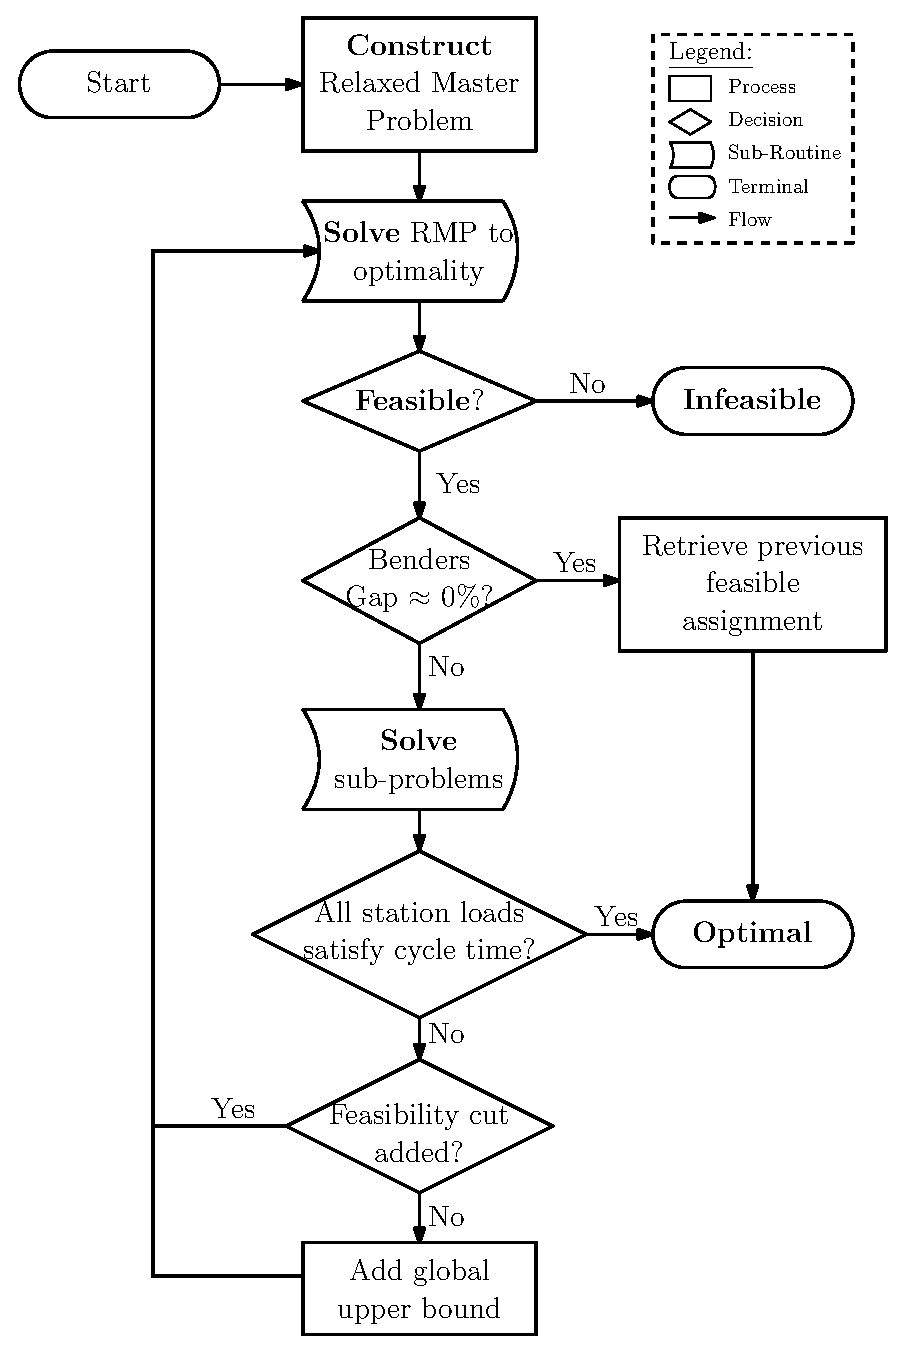
\includegraphics[height=0.95\textheight]{images/Benders-Optimality-Flowchart.eps}
	\label{fig:bend:RMPflowchart}
\end{figure}

\subsection{The Sub-Problem}
\label{sec:bend:algSP}
Once the assignment of tasks to the $m$ stations is found,
all sub-problems are solved.
Unless stated otherwise, we will only consider optimality sub-problems
for the description given here.
We now refer the reader to Figure \ref{fig:bend:SPflowchart}
for an overview of how a single sub-problem is processed.
We first check if the current assignment to the station
has been solved previously or not.
All previous solutions are stored together with their optimal station
load values, so if we find an assignment which has already been processed,
then we retrieve the previous solution and move to the next sub-problem.
In the case of a new assignment of tasks, the sub-problem
is constructed and solved to optimality.

When a sub-problem is found to be infeasible a logic cut
is added; when the load does not satisfy the current cycle time
an infer cut is added; and if the cycle time is satisfied then
no cut is generated.
In all three cases, the resulting solution is stored with
the current assignment for future referral.
The process continues on to the next sub-problem until none remain and
then returns to the master.

\begin{figure}[tbp]
	\centering
	\caption{Flowchart of an optimality sub-problem}
	\vspace{2mm}
	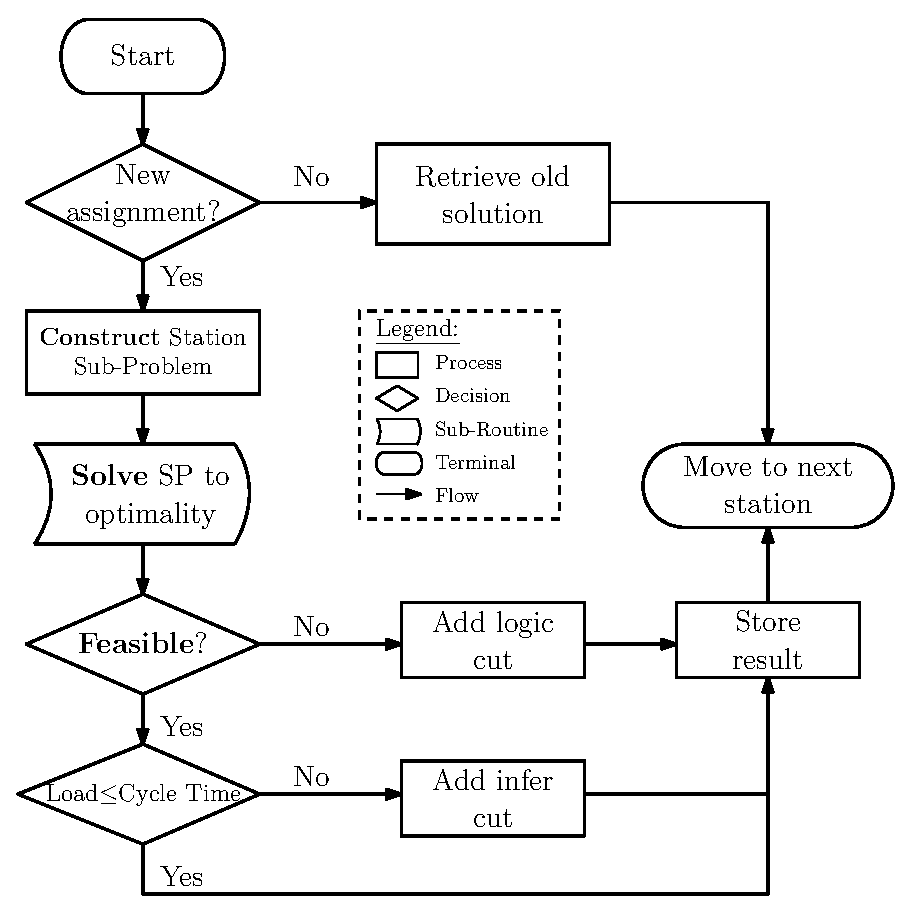
\includegraphics[width=0.95\textwidth]{images/Optimality-SP-Flowchart.eps}
	\label{fig:bend:SPflowchart}
\end{figure}

\subsection{Heuristic Approach}
We conclude this chapter by mentioning a minor modification
that can be made to the above procedure.
We only considered a tolerance of $0\%$ on the Bender
gap, however we could instead take $\varepsilon>0$.
This would result in our exact solution methodology becoming
a heuristic method able to guarantee a pre-defined
quality on the assignment and schedule found.
For example, if we set $\varepsilon=0.05$, then the
algorithm will terminate once a globally feasible solution is found
which is within $5\%$ of the optimal.
The modification of this parameter 
offers this logic-based Benders decomposition
a higher degree of flexibility.
It is possible that reaching a gap of $5\%$ can be done very efficiently
but finding the global optimal is intractable.
In practice, the industry representative
may only require feasible solutions of this quality
as the sub-optimal solution could still be superior to their 
current assembly line design.



%!TEX root = thesis-kdyoung.tex

\chapter{Computational Experiments}
\label{chap:exp}

All experiments were run on a personal computer with
an Intel i5 5575R CPU (four cores each with 2.8GHz clock speed) and 16GB of main memory.
The scripts for the MIPs and the primary script used 
to iterate through the Benders
decomposition algorithm was written in Python 3.4.
We employed Gurobi 7.0.2 as the solver
used for all MIP formulations.
As mentioned previously, \chuffed was the solver
we chose to solve all constraint programs with.
MiniZinc version 2.1.2 was used to compile the models
into the \chuffed FlatZinc format.
Unless stated otherwise, all tests were run
with a time limit of 30 minutes (1800 seconds).

We chose to only test \fsbf{2} and \scbf{2} for the
computational experiments of the previous work.
This is a result of our encoding of the \ssbf{2} model
returning infeasible solutions in our preliminary tests.
Due to time constraints we were unable to discern whether
the problem was our encoding of the model
or if the \ssbf{2} is ill-formed.

We now provide a brief outline of the computational
results reported in this chapter.
First a description of the data used for testing
is given in Section \ref{sec:exp:data}.
As the MIPs presented in \authciteb{Esmaeilbeigi2016}
have been untested, we investigate the best combination
of valid inequalities to include for these models
in Section \ref{sec:exp:mip}.
In Section \ref{sec:exp:cuts} we report on the best combination
of Benders cuts to use for our decomposition.
We provide a detailed investigation into the best configuration
of the CP sub-problem in Section \ref{sec:exp:cp}.
Once the superior sub-problem formulation is determined, 
we close in Section \ref{sec:exp:benchmarkExp} of
this chapter by reporting on the results of our best
solution methodology on a set of benchmark instances.

\section{Data}
\label{sec:exp:data}
The primary dataset available for the \sua{} is
the SBF generated by \citeauthor{Scholl2013}
However, this dataset was created for the type-1 case in
particular and so is not immediately applicable to
the \sua{2}.
The SBF is divided into two halves, the SBF1 and SBF2, 
where each half consists of a total of 1076 instances.
We first provide a brief explanation of how SBF1
was generated.

The basis of the SBF1 are a set of 269 instances
for the \sab{1} containing between 4 and 297 tasks.
When creating instances for the \sua{1}, the cycle time,
task times and precedence relations are all transferred from
the original instances.
We also require values of the forward and backward setup times \ap 
so to create these the authors consider the average processing
time among all tasks, denoted $t_{av}$.
In practice the setup times are smaller than the execution time
of a task, so a parameter $\alpha$ is used when randomly generating
the setups.
An upper bound on the possible setup is defined as $\alpha\cdot t_{av}$
where $\alpha\in\{\:0.25,\:0.50,\:0.75,\:1.00\:\}$.
For example, when $\alpha=1.00$, the largest possible setup time
is 50\% of the average task time.
The 269 input instances are duplicated for each $\alpha$ value
and so 1076 instances of \sua{1} are generated for SBF1.

The SBF2 was generated in almost exactly the same way as SBF1.
However in this case,
care was taken when randomly generating the setup times to ensure
that at least one optimal solution to the original \sab{1} instance
is still feasible in the new \sua{1} instance.
This solution will necessarily be the optimal solution
of the \sua{2} as noted by \citeauthor{Scholl2013}
When storing the instance data, the authors also recorded the
optimal number of stations for the original \sab{1} instance.

The data we chose to run all our tests on was adapted from the SBF2
dataset.
As the optimal solutions were recorded,
we could take the optimal number of stations as input
and then solve for the cycle time.
This simple change allowed 1076 instances for testing our formulations.
\authciteb{Esmaeilbeigi2016} considered a subset of the SBF2 instances
which they divided into 3 classes.
We considered the same subset of instances for the type-2 problem
which are detailed in Table \ref{tab:exp:dataSBF2}.
In this table we give the number of tasks, stations, precedence
relations and order strength of the precedence graph.
In total 396 instances were considered in our tests.

The order strength of an instance is a measure of its complexity
where higher values correspond to more difficult instances.
However, we note that in the extreme, when $OS=1$, there is only one 
precedence-feasible task sequence and thus the problem becomes trivial.

\begin{table}[tpb]
	\centering
	\caption{Dataset summary}
	\vspace{2mm}
	\begin{tabular}{llrrrrr}
		\toprule
		Class & Creator & \#Inst. & $n$ & $m$ & $|E|$ & Order Strength $(OS)$ \\
		\midrule\midrule
		1 &  & 108 & 7-21 & 2-8 & 6-27 & \\[1mm]
		 & {\tt mertens}  & 6 & 7 & 2-6 & 6 & medium (52.40)\\
		  & {\tt bowman8}  & 1 & 8 & 5 & 8 & high (75.00)\\
		  & {\tt jaeschke} & 5 & 9 & 3-8 & 11 & high (83.33)\\
		  & {\tt jackson}  & 6 & 11 & 3-8 & 13 & medium (58.18)\\
		  & {\tt mansoor}  & 3 & 11 & 2-4 & 11 & medium (60.00)\\
		  & {\tt mitchell} & 6 & 21 & 3-8 & 27 & high (70.95)\\\midrule
		2 &  & 112 & 25-30 & 3-14 & 32-40 & \\[1mm]
		  & {\tt roszieg} & 6 & 25 & 4-10 & 32 & high (71.67)\\
		  & {\tt heskia}   & 6 & 28 & 3-8 & 40 & low (22.49)\\
		  & {\tt buxey}    & 7 & 29 & 7-13 & 36 & medium (50.74)\\
		  & {\tt sawyer30} & 9 & 30 & 5-14 & 32 & low (44.83)\\\midrule
		3 &  & 176 & 32-58 & 3-31 & 38-82 & \\[1mm]
		  & {\tt lutz1}   & 6 & 32 & 6-11 & 38 & high (83.47)\\
		  & {\tt gunther}  & 7 & 35 & 7-14 & 43 & medium (59.50)\\
		  & {\tt kilbrid}  & 10 & 45 & 3-10 & 62 & low (44.60)\\
		  & {\tt hahn}     & 5 & 53 & 4-8 & 82 & high (83.82)\\
		  & {\tt warnecke} & 16 & 58 & 14-31 & 70 & medium (59.10)\\\midrule
		Overall & & 396 & 7-58 & 2-31 & 6-82 & \\
		\bottomrule
	\end{tabular}
	\label{tab:exp:dataSBF2}
\end{table}

% \section{Preliminary Tests}
% \label{sec:exp:prelim}

\section{MIP Formulations}
\label{sec:exp:mip}
We first report on how the MIP formulations presented
in Chapter \ref{chap:mip} performed.
In Table \ref{tab:exp:resultsFSBF} and \ref{tab:exp:resultsSCBF} we give the results
of \fsbf{2} and \scbf{2} respectively.
Each is tested on each combination of the valid inequalities from
Section \ref{sec:mip:validIneqs} against
all 3 classes of the subset
of instances from SBF2.
The following datapoints are summarized for each test:
the number of nodes explored by \gurobi's \bab tree,
the average gap for all instances,
the number of instances where no feasible solution was found,
the fraction of instances found to optimality out of the whole class,
the percentage of optimal instances and finally
the average runtime taken by \gurobi.

\begin{table}[tpb]
	\caption{FSBF-2 formulations tested on classes 1,2 and 3}
	\centering
	\vspace{2mm}
	\begin{tabular}{clrrrrrr}
		\toprule
		Class & Ineqs. & \#Nodes & \%Gap & \#No.s. & \#Opt. & \%Opt. & Rt.(s) \\\midrule\midrule
		1 & -- & 40,181 & 0.56 & 0 & 98/108 & 90.74 & 172.90 \\
		 & (\ref{eq:mip:valIneq1}) & 43,437 & 0.16 & 0 & \bf{101}/108 & 93.52 & 166.57 \\
		 & (\ref{eq:mip:valIneq3}) & 50,987 & 1.14 & 0 & 84/108 & 77.78 & 628.47 \\
		 & (\ref{eq:mip:valIneq1}),(\ref{eq:mip:valIneq3}) & 51,734 & 1.12 & 0 & 85/108 & 78.73 & 645.02 \\\midrule
		2 & -- & 171,847 & 14.81 & 0 & 0/112 & 0.00 & 1801.08 \\
		 & (\ref{eq:mip:valIneq1}) & 168,899 & 13.76 & 0 & 0/112 & 0.00 & 1800.66 \\
		 & (\ref{eq:mip:valIneq3}) & 205,752 & 18.04 & 0 & 0/112 & 0.00 & 1801.52 \\
		 & (\ref{eq:mip:valIneq1}),(\ref{eq:mip:valIneq3}) & 202,980 & 17.90 & 0 & 0/112 & 0.00 & 1801.27 \\\midrule
		3 & -- & 48,927 & 19.75 & 9 & 7/176 & 3.98 & 1763.45 \\
		 & (\ref{eq:mip:valIneq1}) & 46,060 & 19.56 & 9 & 7/176 & 3.98 & 1759.67 \\
		 & (\ref{eq:mip:valIneq3}) & 62,845 & 25.64 & 16 & 0/176 & 0.00 & 1800.23 \\
		 & (\ref{eq:mip:valIneq1}),(\ref{eq:mip:valIneq3}) & 63,002 & 24.72 & 15 & 0/176 & 0.00 & 1801.12 \\
		\bottomrule
	\end{tabular}
	\label{tab:exp:resultsFSBF}
\end{table}

\begin{table}[tpb]
	\caption{SCBF-2 formulations tested on classes 1,2 and 3}
	\centering
	\vspace{2mm}
	\begin{tabular}{clrrrrrr}
		\toprule
		Class & Ineqs. & \#Nodes & \%Gap & \#No.s. & \#Opt. & \%Opt. & Rt.(s) \\\midrule\midrule
		1 & -- & 221,842 & 1.62 & 0 & \bf{92}/108 & 86.11 & 374.88 \\
		 & (\ref{eq:mip:valIneq1}) & 244,811 & 1.97 & 0 & 84/108 & 77.78 & 403.17 \\
		 & (\ref{eq:mip:valIneq3}) & 238,515 & 1.75 & 0 & 86/108 & 76.93 & 377.05  \\
		 & (\ref{eq:mip:valIneq1}),(\ref{eq:mip:valIneq3}) & 215,866 & 1.75 & 0 & 86/108 & 76.93 & 380.82  \\\midrule
		2 & -- & 651,880 & 18.01 & 28 & 0/112 & 0.00 & 1800.33 \\
		 & (\ref{eq:mip:valIneq1}) & 701,617 & 19.75 & 31 & 0/112 & 0.00 & 1800.47 \\
		 & (\ref{eq:mip:valIneq3}) & 686,566 & 18.98 & 30 & 0/112 & 0.00 & 1801.03 \\
		 & (\ref{eq:mip:valIneq1}),(\ref{eq:mip:valIneq3}) & 612,442 & 18.57 & 31 & 0/112 & 0.00 & 1800.99 \\\midrule
		3 & -- & 301,055 & 10.09 & 109 & 0/176 & 0.00 & 1800.88 \\
		 & (\ref{eq:mip:valIneq1}) & 326,284 & 12.20 & 117 & 0/176 & 0.00 & 1801.00 \\
		 & (\ref{eq:mip:valIneq3}) & 324,878 & 12.15 & 112 & 0/176 & 0.00 & 1801.21 \\
		 & (\ref{eq:mip:valIneq1}),(\ref{eq:mip:valIneq3}) & 319,908 & 12.06 & 117 & 0/176 & 0.00 & 1801.01 \\
		\bottomrule
	\end{tabular}
	\label{tab:exp:resultsSCBF}
\end{table}

By inspecting the data we find that using the 
valid inequality (\ref{eq:mip:valIneq1})
without (\ref{eq:mip:valIneq3}) is the best 
formulation of \fsbf{2}.
As for \scbf{2}, we found that the best formulation
was when neither of the two valid inequalities were included in
the program.

For both the MIPs, optimality was proven for almost none of the instances of
class 2 and 3.
As a result, all the average runtime values are close
to the time limit of 30 minutes.
In the case of \scbf{2}, no feasible solution was found for 66.5\% of the instances
in class 3.
Even for the smallest class of data, where there is no more
than 21 tasks, neither MIP was able to prove
optimality for all instances.
We note that when calculating the gap value, we only average
the instances where a feasible solution was found.
With a 30 minute time limit, both MIPs could not achieve
an average gap value less than 10\% for class 2 and 3.

Here we tested the full mixed-integer programming approach
on the smallest subset of instances of the SBF2.
The poor results we have found make it clear that these programs
are unsatisfactory exact solution methods for tackling
the \sua{2}.

\section{Cuts}
\label{sec:exp:cuts}
The cutting strategy used in the iteration of the Benders
algorithm can have a large impact on its overall performance.
Even when either the master or sub-problem is exceptionally
difficult to solve, if the Benders cuts added to the master
allow us to find optimality in very few iterations then the problem
can still be tractable.

\subsection{Nogood Cuts}
\label{sec:exp:NGcuts}
In the preliminary testing phase, we considered feasibility sub-problems
using the nogood cuts presented in Section \ref{sec:bend:NGcuts} of the 
previous chapter.
These results are briefly summarized in Table \ref{tab:exp:resultsNGcut}.
Even on the smallest class 1, the Benders
algorithm failed to prove optimality for 66 of the instances tested.
Due to this, we felt that further investigation into the use
of nogood cuts was not the most fruitful research direction. 
Note that we did not make use of the possible parallel computing capabilities
detailed earlier in Section \ref{sec:bend:SPfeas},
where the feasibility sub-problems could be run concurrently.
This potential avenue was not explored as the percentage of computation
time spent solving the sub-problems was dwarfed by the time spent solving
the master problem; as we will see in the coming results.

For all remaining experiments optimality sub-problems were used
unless stated otherwise.

\begin{table}[tpb]
	\caption{Benders algorithm tested on class 1 with nogood cuts}
	\centering
	\vspace{2mm}
	\begin{tabular}{ccrrrr}
		\toprule
		Cuts & Class & \#No sol. & \#Opt. & \%Opt. & Runtime(s) \\\midrule\midrule
		$\mathcal{C}_{ng}$ & 1 & 66 & 42/108 & 38.89 & 1456.57 \\
		\bottomrule
	\end{tabular}
	\label{tab:exp:resultsNGcut}
\end{table}

\subsection{Cutting Procedure}
\label{sec:exp:cuttngProcedure}
In Tables \ref{tab:exp:resultsCutsClass1} and \ref{tab:exp:resultsCutsClass2}
we provide the primary comparison of the possible cutting strategies
that we considered.
The first table compares the 9 possible cut combinations on the smallest
class of data (class 1).
The variation in the results of Table \ref{tab:exp:resultsCutsClass1},
makes it difficult to discern a
clear best cutting procedure.
So we further tested 6 cut combinations
on class 2 in the Table \ref{tab:exp:resultsCutsClass2}.
The choice of solving technology for the sub-problems 
will only effect the time taken to solve all scheduling problems
but not the cutting procedure.
Thus we arbitrarily chose to test all combinations of cuts using MIP
sub-problems.

The two tables comparing the cut combinations contain
the following data:
average number of nodes explored by \gurobi's
\bab tree (total combined between the \rmp{} and sub-problems),
average number iterations of the Benders algorithm,
average number of cuts generated,
average Benders gap,
total number of instances where no feasible solution was found,
percentage of the instances proved optimal and
the average runtime of all instances.

By inspecting the results of Table \ref{tab:exp:resultsCutsClass1}
it is difficult to reason about which cutting strategy is superior
as all instances were proved optimal for every combination.
These results immediately tell us that the Benders decomposition
we present here has outperformed the pure MIP formulations
previously presented by the literature.
We note that when the global bound in not enforced after
a globally feasible solution is found, the Benders gap
remains substantially large and so it is difficult
to measure the convergence of the Benders algorithm.
Thus for the remaining experiments we run, the global bound
will always be used unless stated otherwise.
The $3^{\text{rd}}$ version of the inference cut ($\mathcal{C}_{iii}$) appears to
be a key ingredient in the Benders algorithm terminating efficiently,
but to confirm this suspicion we test our solution
methodology on class 2.

\begin{table}[tpb]
	\caption{Benders cutting strategies compared on class 1}
	\centering
	\vspace{2mm}
	\begin{tabular}{cccccrrrrrrr}
		\toprule
		\multicolumn{5}{c}{Cuts and Bound}  &  &  &  &  &  &  &   \\\cmidrule(rl){1-5}
		$\mathcal{C}_{i}$ & $\mathcal{C}_{ii}$ & $\mathcal{C}_{iii}$ & $\mathcal{C}_{l}$ & $\mathcal{C}_{gb}$& \#Nodes & \#Its. & $|\mathcal{C}|$ & \%Gap & \#No.s. & \%Opt. & Rt.(s) \\\midrule\midrule
		\checkmark &  &  &  &  & 4,718 & 18 & 35 & 0.00 & 0 & 100.00 & 5.8 \\
		 & \checkmark &  &  &  & 2,845 & 15 & 28 & 0.00 & 0 & 100.00 & 4.1 \\
		 &  & \checkmark &  &  & 170 & 4 & 8 & 0.00 & 0 & 100.00 & 1.1 \\\midrule
		\checkmark &  &  &  & \checkmark & 3,790 & 16 & 32 & 0.00 & 0 & 100.00 & 2.9 \\
		 & \checkmark &  &  & \checkmark & 2,064 & 12 & 26 & 0.00 & 0 & 100.00 & 1.9 \\
		 &  & \checkmark &  & \checkmark & 128 & 3 & 9 & 0.00 & 0 & 100.00 & 0.4 \\\midrule
		\checkmark &  &  & \checkmark & \checkmark & 766 & 17 & 34 & 0.00 & 0 & 100.00 & 2.6 \\
		 & \checkmark &  & \checkmark & \checkmark & 896 & 17 & 34 & 0.00 & 0 & 100.00 & 2.8 \\
		 &  & \checkmark & \checkmark & \checkmark & 56 & 4 & 12 & 0.00 & 0 & 100.00 & 0.5 \\
		\bottomrule
	\end{tabular}
	\label{tab:exp:resultsCutsClass1}
\end{table}

In Table \ref{tab:exp:resultsCutsClass2} we can see that
class 2 proved more challenging for the Benders decomposition
to solve the problem as in many cases optimality was
proven for only $\sim30\%$ of the instances.
These results make it clear that $\mathcal{C}_{iii}$
is the strongest infer cut as it is able to
solve almost twice as many instances to optimality
that the other 2 infer cuts.
Further to this, it needed half as many iterations
and similarly half as many cuts in total.
For the instances where the optimal solution was not found,
$\mathcal{C}_{iii}$ provided the lowest Benders gap values
as well.

We must also examine whether including the logic cut, $\mathcal{C}_{l}$,
provided a benefit.
When considering the logic cut, a global bound on the cycle time is instituted
as an upper bound on the load of each station's sub-problem,
possibly leading to feasibility sub-problems, rather than optimality.
The logic cut was formulated to provide the \rmp{} with detailed information
about the assignment variables whilst also reducing the time
needed to solve a sub-problem; however it also has a notable drawback.
When a logic cut is generated by a sub-problem, that sub-problem
has not been solved to optimality.
This results in us not being able to generate an optimality cut for
this sub-problem, such as $\mathcal{C}_{iii}$.
The results of Table \ref{tab:exp:resultsCutsClass2} indicate
that on average, not being able to perform an infer cut has not outweighed the beneficial
information provided by the logic cut.

\begin{table}[tpb]
	\caption{Benders cutting strategies compared on class 2}
	\centering
	\vspace{2mm}
	\begin{tabular}{cccccrrrrrrr}
		\toprule
		\multicolumn{5}{c}{Cuts and Bound}  &  &  &  &  &  &  &   \\\cmidrule(rl){1-5}
		$\mathcal{C}_{i}$ & $\mathcal{C}_{ii}$ & $\mathcal{C}_{iii}$ & $\mathcal{C}_{l}$ & $\mathcal{C}_{gb}$ & \#Nodes & \#Its. & $|\mathcal{C}|$ & \%Gap & \#No.s. & \%Opt. & Rt.(s) \\\midrule\midrule
		\checkmark &  &  &  & \checkmark & 1,522k & 99 & 396 & 11.63 & 1 & 31.25 & 1339.7 \\
		 & \checkmark &  &  & \checkmark & 1,430k & 99 & 399 & 10.79 & 1 & 32.14 & 1348.5 \\
		 &  & \checkmark &  & \checkmark & 1,024k & 47 & 196 & 8.42 & 1 & \bf{60.71} & 959.9 \\\midrule
		\checkmark &  &  & \checkmark & \checkmark & 918k & 112 & 439 & 11.38 & 1 & 33.04 & 1318.4 \\
		 & \checkmark &  & \checkmark & \checkmark & 964k & 114 & 443 & 11.33 & 1 & 31.25 & 1342.3 \\
		 &  & \checkmark & \checkmark & \checkmark & 898k & 68 & 225 & 9.03 & 1 & 58.04 & 956.8 \\
		\bottomrule
	\end{tabular}
	\label{tab:exp:resultsCutsClass2}
\end{table}

Hence, for all remaining experiments we used the infer cut $\mathcal{C}_{iii}$
in combination with the global bound $\mathcal{C}_{gb}$ as the cutting
procedure, unless stated otherwise.

We mention here that combining different 
types of infer cuts together in a single cutting procedure
was not explored.
This is because every inference made by $\mathcal{C}_{i}$ is 
contained within $\mathcal{C}_{ii}$ and every inference made by $\mathcal{C}_{ii}$
is similarly contained within $\mathcal{C}_{iii}$.
Thus combining these infer cuts will not lead to a
substantial reduction in runtime.

% \begin{table}[tpb]
% 	\begin{adjustwidth}{-.9in}{-.9in}
% 	\caption{Benders cutting strategies compared on classes 1 and 2}
% 	\centering
% 	\vspace{2mm}
% 	\begin{tabular}{ccrrrrrrrrrrr}
% 		\toprule
% 		Cuts & Class & \#Nodes & Iters. & \#Cuts & Cuts & \%Gap & \#No sol. & \#Opt. & \%Opt. & Runtime(s) \\\midrule\midrule
% 		$i$ 			& 1 & 4,718 & 18 & 35 & [0,\:0,\:35,\:0,\:0,\:0] & 317.78 & 0 & 108/108 & 450.00 & 5.04 & 0.66 & 5.75 \\
% 						& 2 & 1,437,019 & 103 & 403 & [0,\:0,\:403,\:0,\:0,\:0] & 665.11 & 1 & 35/112 & 218.75 & 1231.88 & 137.11 & 1369.40 \\\midrule
% 		$ii$ 			& 1 & 2,845 & 15 & 28 & [0,\:0,\:0,\:28,\:0,\:0] & 317.78 & 0 & 108/108 & 450.00 & 3.55 & 0.49 & 4.09 \\
% 						& 2 & 1,489,391 & 96 & 383 & [0,\:0,\:0,\:383,\:0,\:0] & 692.04 & 1 & 32/112 & 200.00 & 1146.54 & 213.58 & 1360.52 \\\midrule
% 		$iii$ 			& 1 & 170 & 4 & 8 & [0,\:0,\:0,\:0,\:8,\:0] & 317.37 & 0 & 108/108 & 450.00 & 0.95 & 0.07 & 1.07 \\
% 						& 2 & 1,145,053 & 44 & 184 & [0,\:0,\:0,\:0,\:184,\:0] & 683.09 & 1 & 65/112 & 406.25 & 812.48 & 185.57 & 998.46 \\\midrule
% 		$gb,i$ 			& 1 & 3,790 & 16 & 32 & [0,\:1,\:31,\:0,\:0,\:0] & 15.76 & 0 & 108/108 & 450.00 & 2.31 & 0.58 & 2.93 \\
% 						& 2 & 1,522,487 & 99 & 396 & [0,\:3,\:392,\:0,\:0,\:0] & 11.63 & 1 & 35/112 & 218.75 & 1177.86 & 161.47 & 1339.74 \\\midrule
% 		$gb,\:ii$ 		& 1 & 2,064 & 12 & 26 & [0,\:1,\:0,\:25,\:0,\:0] & 16.01 & 0 & 108/108 & 450.00 & 1.45 & 0.38 & 1.88 \\
% 						& 2 & 1,430,956 & 99 & 399 & [0,\:3,\:0,\:396,\:0,\:0] & 10.79 & 1 & 36/112 & 225.00 & 1136.87 & 211.25 & 1348.53 \\\midrule
% 		$gb,\:iii$ 		& 1 & 128 & 3 & 9 & [0,\:1,\:0,\:0,\:7,\:0] & 16.09 & 0 & 108/108 & 450.00 & 0.30 & 0.06 & 0.41 \\
% 						& 2 & 1,024,879 & 47 & 196 & [0,\:3,\:0,\:0,\:192,\:0] & 8.42 & 1 & 68/112 & 400.00 & 786.47 & 173.05 & 959.93 \\\midrule
% 		$gb,\:i,\:lc$ 	& 1 & 766 & 17 & 34 & [0,\:1,\:14,\:0,\:0,\:19] & 15.80 & 0 & 108/108 & 450.00 & 2.01 & 0.54 & 2.60 \\
% 						& 2 & 918,423 & 112 & 439 & [0,\:3,\:209,\:0,\:0,\:227] & 11.38 & 1 & 37/112 & 231.25 & 1175.16 & 142.86 & 1318.43 \\\midrule
% 		$gb,\:ii,\:lc$ 	& 1 & 896 & 17 & 34 & [0,\:1,\:0,\:13,\:0,\:20] & 15.88 & 0 & 108/108 & 450.00 & 2.15 & 0.55 & 2.76 \\
% 						& 2 & 964,875 & 114 & 443 & [0,\:3,\:0,\:204,\:0,\:236] & 11.33 & 1 & 35/112 & 218.75 & 1199.93 & 141.94 & 1342.29 \\\midrule
% 		$gb,\:iii,\:lc$ & & 128 & 3 & 9 & [0,\:1,\:0,\:0,\:7,\:0] & 16.09 & 0 & 108/108 & 450.00 & 0.30 & 0.06 & 0.41 \\
% 						& 2 & 1,024,879 & 47 & 196 & [0,\:3,\:0,\:0,\:192,\:0] & 8.42 & 1 & 65/112 & 400.00 & 786.47 & 173.05 & 959.93 \\
% 		\bottomrule
% 	\end{tabular}
% 	\label{tab:exp:resultsCuts}
% 	\end{adjustwidth}
% \end{table}

\section{CP Sub-Problem}
\label{sec:exp:cp}
The CP solver \chuffed provides the
user with numerous input parameters to
tailor the propagation and search procedure 
to the problem at hand.
In this section, we report on the comparisons
between the model formulation
and search strategies in order to find the best suited
configuration for the \sua{2} instances.

As we are only concerned with optimizing the sub-problems'
solving time, the runtime values we present here will
only average the time used by the CP model, 
\ie excluding the runtime of the master problem.
Similarly, this also applies to the average number of nodes
explored by the CP sub-problems..

% \todo{once the best is found we will use this procedure for all
% remaining experiments (unless stated otherwise, in the
% case of testing the upper-bound cuts with the CP sub-problem).}

% global upper bound:

% The upper bound cut reduces the space complexity of the sub-problems
% very helpful for cp solver whose difficultly is very closely
% related to the inference that can be done on the finite domains. 

% \todo{mention how the formulation performed when
% global upper bound was removed. ... badly. why?
% because cp could not handle such large domains of the
% variables.}

\subsection{Model Formulation}
\label{sec:exp:cpForm}
Two main types of CP models were considered, so we
first check which of these is superior before moving
on to test other input parameters.
$CP_1$ represents the model detailed in Section \ref{sec:bend:cpModel}
from the previous chapter.
$CP_2$ represents the same model but with the additional decision
variable $\sigma_{ij}$ and the \cumu global constraint.

In Table \ref{tab:exp:resultsCPmodel}, we compare these two models 
against each other on the class 1 and
class 2 instances where $\alpha$ is fixed to $1.00$.
The search strategy used for these tests was simply the default
search of \chuffed.
These tests indicate that there is a reduction
in sub-problem runtime when the \cumu constraint
is used in the CP formulation.
For all remaining experiments where CP sub-problems
were used, $CP_2$ was the formulation utilized
unless stated otherwise.

\begin{table}[tpb]
	\caption{CP formulations compared on classes 1 and 2 when $\alpha=1.00$}
	\centering
	\vspace{2mm}
	\begin{tabular}{ccrrrrrr}
		\toprule
		Class & Model & \#SP Nodes & \%Gap & \%Opt. & SP Runtime(s) \\\midrule\midrule
		1 & $CP_1$ & 32,755 & 0.00 & 100.00 & 3.83  \\
		 & $CP_2$ & 29,225 & 0.00 & 100.00 & \bf{2.84} \\\midrule
		2 & $CP_1$ & 2,768,871 & 15.45 & 25.00 & 386.71 \\
		 & $CP_2$ & 2,503,183 & 14.03 & 25.00 & \bf{329.60} \\
		\bottomrule
	\end{tabular}
	\label{tab:exp:resultsCPmodel}
\end{table}

% \begin{table}[tpb]
% 	\caption{Input parameters of CP}
% 	\centering
% 	\vspace{2mm}
% 	\begin{tabular}{cccccrrrrrrr}
% 		\toprule
% 		\multicolumn{3}{c}{Parameters}  &  &  &  &  &  &  &   \\\cmidrule(rl){1-3}
% 		{\tt -f} & {\tt tt} & {\tt ttef} \#Nodes & \#Its. & $|\mathcal{C}|$ & \%Gap & \#No.s. & \%Opt. & Rt.(s) \\\midrule\midrule
% 		 &  &  & 1,522k & 99 & 396 & 11.63 & 1 & 31.25 & 1339.7 \\
% 		 &  &  & 1,430k & 99 & 399 & 10.79 & 1 & 32.14 & 1348.5 \\
% 		 &  &  & 1,024k & 47 & 196 & 8.42 & 1 & 60.71 & 959.9 \\\midrule
% 		 &  &  & 918k & 112 & 439 & 11.38 & 1 & 33.04 & 1318.4 \\
% 		 &  &  & 964k & 114 & 443 & 11.33 & 1 & 31.25 & 1342.3 \\
% 		 &  &  & 898k & 68 & 225 & 9.03 & 1 & 58.04 & 956.8 \\
% 		\bottomrule
% 	\end{tabular}
% 	\label{tab:exp:resultsCPparameters}
% \end{table}


\subsection{Search Strategy}
\label{sec:exp:cpSearch}
Earlier in Section \ref{sec:bend:cpForm}
of the previous Chapter, we detailed a range of possible search procedures
which could be employed when solving our constraint program.
In Table \ref{tab:exp:resultsCPsearch} we present the results
of testing the CP sub-problems on a selection of these procedures.
The names of the searches refer to the following procedures:
{\tt def} is the default search, {\tt start} is the basic search on start time variables,
{\tt start\_ff\_Then\_sigma} is a sequential search of start then $\sigma$ variables. 
Four priority searches were considered which only differ by the variable selection
strategy used to choose the next sequential procedure.
% ; these are 
% {\tt priority\_io} using {\tt input\_order} variable selection, 
% {\tt priority\_sm} using {\tt smallest},
% {\tt priority\_sml} using {\tt smallest\_largest} and
% {\tt priority\_ff} using {\tt first\_fail}.

From the results of Table \ref{tab:exp:resultsCPsearch}, 
we can immediately conclude that the default search
is inferior to the search strategies we have tailored for
the \sua{2}.
Although, among the search procedures we devised, there
is very little variations in the results.
Each procedure was able to find the optimal solution
for the same number of instances,
while the runtime was very similar.
The basic search {\tt start} needed to explore the fewest
number of nodes in the search tree, however the priority search
{\tt priority\_ff} provided the best average runtime.
For all remaining tests where CP sub-problems
were utilized, the priority based search strategy using 
the {\tt first\_fail} variable selection was used.


\begin{table}[tpb]
	\caption{CP search strategies compared on class 2 when $\alpha=1.00$}
	\centering
	\vspace{2mm}
	\begin{tabular}{clrrrrrr}
		\toprule
		Class & Search & \#SP Nodes & \%Gap & \%Opt. & SP Runtime(s) \\\midrule\midrule
		2 & {\tt default}			& 2,503k & 14.03 & 25.00 & 329.60 \\
		 & {\tt start}				& 1,884k & 8.97 & 42.86 & 246.57 \\
		 & {\tt start\_ff\_Then\_sigma}	& 2,391k & 9.69 & 42.86 & 254.23 \\
		 & {\tt priority\_io}		& 2,448k & 9.12 & 42.86 & 253.70 \\
		 & {\tt priority\_sm}		& 2,408k & 9.06 & 42.86 & 252.91 \\
		 & {\tt priority\_sml}		& 2,470k & 9.04 & 42.86 & 252.63 \\
		 & {\tt priority\_ff}		& 2,426k & 8.90 & 42.86 & \bf{245.74} \\
		\bottomrule
	\end{tabular}
	\label{tab:exp:resultsCPsearch}
\end{table}

\section{Benchmark Experiments}
\label{sec:exp:benchmarkExp}
We close this chapter by comparing the best
configuration of our logic-based Benders decomposition
against the results of the MIP formulations for all benchmark
instances from the subset of SBF2 we have used.
Before presenting this final result, we must first
decide on the best sub-problem formulation for our
Benders decomposition.

Earlier in Section \ref{sec:lit:cpChuffed}, we gave a
brief description of the CP solver, \chuffed, we chose to utilize when
tackling the constraint programs we formulated.
As mentioned in that section, \chuffed does not currently have
the ability to be run in parallel.
This handicap has hampered its ability to effectively compete
with \gurobi, which can easily run in parallel on all four cores
of the computer we used for testing.

In Table \ref{tab:exp:resultsSPform} we present a comparison
of our Benders decomposition algorithm tested on the class 2
instances when using MIP and CP sub-problems.
There are many more nodes explored when using CP sub-problems
due to the different search procedure of a CP solver
when compared to a MIP solver.
The results of the two formulations are similar, but we can
conclude that our best configuration of the CP model
has provided a reduction in runtime when compared to the MIP
formulation.

\begin{table}[tpb]
	\caption{MIP and CP sub-problem formulations compared on class 2}
	\centering
	\vspace{2mm}
	\begin{tabular}{ccrrrrrr}
		\toprule
		Class & Sub-Problem & \#SP Nodes & \%Gap & \%Opt. & SP Runtime(s) \\\midrule\midrule
		2 & \spmip{} & 630k & 8.42 & 60.71 & 173.05 \\
		 & \spcp{} & 2,489k & 8.21 & 61.61 & \bf{165.26} \\
		\bottomrule
	\end{tabular}
	\label{tab:exp:resultsSPform}
\end{table}

Now using the best formulation of our Benders decomposition
we present the results of our final benchmark experiments 
on all 3 classes from the subset of the SBF2 instances.
These results can be found in Table \ref{tab:exp:resultsBestBenders}
where we provide the average number of iterations,
cuts, average gap, number optimal and runtime breakdown.
The instances from classes 2 and 3 proved to be more
challenging than the smaller instances from class 1.
Most notably, the total runtime taken by
the Benders algorithm is almost entirely due to the complexity of the \rmp{}.

More cuts are to be expected when the difficultly of the problem
is increased, but we also mention that for the instances of class 3
there is also a larger number of stations.
This will lead to more cuts being made for every iteration of the algorithm.

\begin{table}[tpb]
	\caption{Benchmark results of our final Benders decomposition}
	\centering
	\vspace{2mm}
	\begin{tabular}{crrrrrr}
		\toprule
		Class & \#Its. & \#Cuts. & \%Gap & \#Opt. & RMP.Runtime(s) & SP.Runtime(s) \\\midrule\midrule
		1 & 3 & 9 & 0.00 & 108/108 & 0.36 (87.95\%) & 0.04 (10.98\%) \\
		2 & 47 & 196 & 8.21 & 69/112 & 781.29 (82.33\%) & 165.26 (17.42\%) \\
		3 & 92 & 468 & 15.76 & 27/176 & 1462.01 (88.00\%) & 173.63 (10.45\%) \\
		\bottomrule
	\end{tabular}
	\label{tab:exp:resultsBestBenders}
\end{table}

Table \ref{tab:exp:resultsBenchmark} compares how our final results perform
when compared to the pure MIP formulations of the \sua{2}.
For each class of instances our solution methodology beats the best formulation
of the MIPs.
In the case of class 2 where the Benders decomposition could not prove optimality for
all instances, the average Benders gap at termination is superior to
the best average gap found by \gurobi when solving either \fsbf{2} and \scbf{2}.
For class 3, our algorithm could only find the optimal solution for 15.3\% of the 176 instances.
Also the \scbf{2} model returned superior average gap values for class 3, even though
it was unable to find any optimal solutions.
Although the gap value of \scbf{2} for the class 3 instances
may be misleading, as it only calculated from
the 59 of 176 instances where a feasible solution was found.

\begin{table}[tpb]
	\caption{Benders decomposition compared to pure MIP formulations}
	\centering
	\vspace{2mm}
	\begin{tabular}{crrrrrrrr}
		\toprule
		 & \multicolumn{4}{c}{Benders decomposition}  & \multicolumn{2}{c}{\fsbf{2}} & \multicolumn{2}{c}{\scbf{2}}  \\
		 \cmidrule(lr){2-5} \cmidrule(lr){6-7} \cmidrule(lr){8-9}
		Class & \%Gap & \#Opt. & \%Opt. & Rt.(s) & \%Gap & \%Opt. & \%Gap & \%Opt. \\\midrule\midrule
		1 & 0.00 & 108/108 & 100.00 & 0.41 & 0.16 & 93.52 & 1.62 & 77.78 \\
		2 & 8.21 & 69/112 & 61.61 & 948.93 & 13.76 & 0.00 & 18.01 & 0.00 \\
		3 & 15.76 & 27/176 & 15.34 & 1661.93 & 19.56 & 3.98 & 10.09 & 0.00 \\
		\bottomrule
	\end{tabular}
	\label{tab:exp:resultsBenchmark}
\end{table}

Our results indicate that the \sua{2} is a difficult problem to solve
when the instance size becomes large.
However, we can see from these results that decomposing the problem using a 
logic-based Benders decomposition framework provides
the most optimal solutions when compared to the other available exact
solution procedures.

% \section{Summary}
% \label{sec:exp:summary}

% blah


% Conclusion
%!TEX root = thesis-kdyoung.tex

% \begin{savequote}%[45mm]
% ---Essentially, all models are wrong, but some are useful.
% \qauthor{George Box}
% \end{savequote}

\chapter{Conclusion}
\label{chap:conc}

In this thesis we devised a logic-based Benders decomposition
of the \sua{2}.
The natural division between the assignment and scheduling
variables led us to believe that this approach would be
well-suited to the problem.
Our formulation resulted in a classical \sab{2}
being solved by the master problem while
a sub-problem for each station was created.
We considered multiple ways of formulating and solving the sequencing
problems that arose in each station.

Logic-based Benders decomposition allowed us to 
formulate a sub-problem as either a MIP or a constraint program and 
using its inference dual to generate Bender cuts.
Employing CP solving technology resulted in marginal
improvements to the runtime and solution quality when compared
to MIP sub-problems.
However the CP solver \chuffed was only able to 
operate on one core while the MIP solver \gurobi was able to utilize
all four cores.
The inclusion of the global constraint \cumu in the CP model
and investigating the possible search strategies of the CP solver,
both contributed to the CP model outperforming the
MIP sub-problem formulation.

Both feasibility and optimality Benders cuts were devised.
Solving each sub-problem to optimality allowed a much wider
range of cuts to be generated at each iteration of the Benders
algorithm.
We provided a detailed analysis into the advantages and disadvantages
of each possible cutting procedure and after performing experiments,
we were able to conclude that combining the global upper bound, $\mathcal{C}_{gb}$,
with our strongest inference cut, $\mathcal{C}_{iii}$, resulted
in the most effective cutting planes added to the relaxed master problem.

In summary, our decomposition approach was able to solve
100\% of the smallest class of instances in an average runtime of
0.41 seconds.
For the second class, which contained small-to-medium sized instances,
our method was able to solve 61.6\% of the instances, while also
finding superior gap values compared to pure MIP models solved with \gurobi.
In the case of largest class we considered, only 15.3\% of optimal solutions
were proven in the 30 minute time limit.
Of the 396 instances we tested which had up to 58 tasks and 31 stations,
the Benders decomposition was able to solve 51.5\% to optimality.

\section{Future Work}
\label{sec:conc:future}
The work and results we have reported on in this thesis
stand as only the very beginning of the research which
could be done into decomposition approaches to the \sua{}.
The logic-based Benders decomposition we devised can be viewed
simply as a framework for a solution procedure to this problem.
As such this framework presents a range of possible future research directions;
some of which we will now detail.

Firstly, applying our Benders decomposition to the type-1 problem
of \sua{} is a straight forward extension.
This will result in $m$ sub-problems needing to be solved
where $m$ is a variable, while each station has an upper bound
on its load.
We can again view these sequencing problems as asymmetric TSPs, however
now not only is the number of cities within each TSP unknown,
but the number of TSPs to be solved is also a decision.
As each sub-problem has a pre-defined upper bound, feasibility
cuts may be better suited in the type-1 case.

The final results we presented in the previous chapter tell us that
the vast majority of solve time in our decomposition is due to
the relaxed master problem.
We only considered a full mixed integer programming approach for the 
master however this was not exclusively necessary. 
Any procedure which can return an assignment of tasks to the stations and provides 
a lower bound on the cycle time would be applicable.
Thus, developing heuristic procedures to replace our current formulation of
the \rmp{} may be a fruitful direction of investigation.
In fact, it is very possible that implementing such a procedure --- even if it is 
relatively simple --- could significantly improve the results 
found here.

In this thesis, we considered few ways of formulating the MIP
version of the sub-problems.
Further investigation into valid inequalities of this program
or simply a different set of decision variables could lead
to better results.
Regarding the CP sub-problems, the lack of parallelization
of the \chuffed solver hindered its capabilities somewhat.
So when this feature becomes available, re-running the
experiments to check the reduction in runtime 
would provide a useful comparison between different
solution technologies.

Finally, we emphasise the limited amount of research which
has been done into the \sua{}.
This variant of the \albp{} presents a non-trivial layer of complexity
with a set of scheduling decisions,
however this consideration is applicable to a wide variety of assembly lines.
Thus, including setup costs in other well-known variants of the 
\albp{} would lead to a range of possible research directions.

% Testing the last MIP formulation. The SSBF-2 formulation of the 
% problem was not tested in this paper and so future work inspecting 
% its capabilities as compared to the other MIPs and the Benders decomposition may provide better results.

% One direction of research which was considered during the Masters
% course but was never explored was the use of some sub-tour-elimination
% constraints within the master.
% This may not be the most fruitful research direction as it adds more 
% information and thus layers of complication to the master problem, 
% which is already the bottleneck of the computational load. 
% Even so, investigating if adding information to the master in the form 
% of callbacks to the solver or constraints to eliminate different
% sizes of sub-tours could result in overall less master 
% problems being required to be solved. 
% Thus it is possible that such an inclusion could reduce the overall 
% computation time of the Benders decomposition.

% Improving the constraint programming sub problem. 
% This could be done in variety of ways. 
% The limitation preventing the use of parallelized search for the constraint 
% programming solver we chose proved to be a non-trivial handicap when compared 
% to Gurobi.
% Recent work in this area indicates that this limitation could soon be 
% removed and investigating the improvement which this results in 
% could be a fruitful direction of research.

% Further to this, our formulation of the sub-problems did not take advantage 
% of the expressive nature of the constraint programming language. 
% Considering an entirely different formulation with ordering 
% decision variables between each pair of tasks could be one possible 
% direction which might be better served by the global scheduling 
% constraints that are well-studied and provide effective propagation.

% In our decomposition we exclusively investigated the quality of optimality sub-problems. 
% However there is very good reason to believe that formulating the Benders 
% decomposition with feasibility sub-problems could also perform very well on this problem. 
% In this case CP sub-problems should be vastly superior to 
% MIP sub-problems due to their inherent advantage of domain 
% propagation to efficiently detect infeasibility.

% Extending this problem by combining it with other variants of the ALBP.
% In particular, the initial motivation we had for investigating the 
% ALBP with setup times was in the case of a multi-skilled workforce. 
% These variants of the ALBP, the ALWABP or ALWIBP, can easily have 
% their decisions incorporated into the master problem. 
% Investigating how the Benders decomposition performs on this extension 
% may be an interesting extension which could be applied to real-world 
% scenarios where the setup costs between tasks not only depend on the 
% tasks in question but also the workers assigned those tasks.

% \todo{define the ALWABP and ALWIBP}

% Consider a CP model based on the scheduling-based MIP presented by
% \authcite{Esmaeilbeigi2016}.
% Adapting their model to make use of global constraints
% and considering different search strateies
% could be fruitful as it would
% allow us to take full advantage of CP's appreciable
% performance on a range of scheduling problems.



%---------------------------------------------------------- 
% APPENDICES
% include chapters as needed (will be numbered differently)
%---------------------------------------------------------- 
\appendix

\chapter{Appendix}

\begin{algorithm}[H]
	\caption{Branch-and-Bound algorithm for a minimization problem}
	\label{alg:lit:bab}
	\begin{algorithmic}[1]
		\Statex
		\State $Incumbent=\infty$
		\State Initialize the tree with root node, $n_0$, and solve the relaxed LP
		% \Let{$BestBound$}{LP solution}
		\Let{$Nodes$}{$\{n_0\}$} \Comment{\emph{The set of nodes to be fathomed}}
		\Statex
		\While{$Nodes\neq \emptyset$}
			\State Select a node $n\in Nodes$
			\State Choose a relaxed variable, $x_i$, in the LP solution
			\State Branch on $x_i$, splitting its domain into two subsets, creating nodes $n_a$, $n_b$
			\State Solve the two relaxed LPs of each node.
			\For{$n_{new} \in \{n_a, n_b\}$}
				\If{$LPsol$ is integer}
					\If{$LPsol < Incumbent$}
						\Let{$Incumbent$}{$LPsol$} \Comment{\emph{Found new best solution}}
					\ElsIf{$LPsol \geq Incumbent$}
						\Let{$Nodes$}{$Nodes\cup\{n_{new}\}$}
					\EndIf
				\ElsIf{$LPsol$ is not integer}
					\If{$LPsol \leq BestBound$}
						\Let{$Nodes$}{$Nodes\cup\{n_{new}\}$}
					\ElsIf{$LPsol > BestBound$}
						\Let{$Nodes$}{$Nodes\setminus\big(n_{new}\cup Children(n_{new})\big)$} \Comment{\emph{Pruning}}
						\State Continue to next node
					\EndIf
				\EndIf
				\If{$LPsol < BestBound$}
					\Let{$BestBound$}{$LPsol$}
				\EndIf
				% \State Current node is fathomed
			\EndFor
		\EndWhile
		\Statex
		\State \Return $Incumbent$
	\end{algorithmic}
\end{algorithm}

\begin{lstlisting}[caption={Full MiniZinc model for CP sub-problems},label={lst:appen:CPmodel},language=minizinc]
% Constraint Programming model for a station's sub-problem
include "cumulative.mzn";
include "disjunctive.mzn";
include "redefinitions.mzn";
%~~~~~~~~~~~~~~~~~~~~~~~~~~~~~~~~~~~~~~~~~~~~~~~~~~~~~~~~~~~~~~~~~~~~~~~~~~~~~~~%
% INSTANCE INITIALISATION
int: nTasks;
int: nPrecs;
int: maxLoad;  % maximum makespan
set of int: TASK;
set of int: PREC = 1..nPrecs;
set of int: TIME = 0..maxLoad;
array[TASK] of int: dur; % duration
array[TASK] of set of TASK: suc; % set of successors
array[TASK,TASK] of int: forwSU; % forward setup times
array[TASK,TASK] of int: backSU; % backward setup times
array[TASK] of set of TASK: followForw; % allowed followers in forward load
array[TASK] of set of TASK: followBack; % allowed followers in backward load
array[TASK] of set of TASK: precedeForw; % allowed preceders in forward load
array[TASK] of set of TASK: precedeBack; % allowed preceders in backward load
%~~~~~~~~~~~~~~~~~~~~~~~~~~~~~~~~~~~~~~~~~~~~~~~~~~~~~~~~~~~~~~~~~~~~~~~~~~~~~~~%
% DECISION VARIABLES
array[TASK] of var TIME: s; % start time
array[TASK,TASK] of var TIME: spair; % start time pairings
array[TASK,TASK] of var bool: y; % forward direction following
array[TASK,TASK] of var bool: z; % backward direction following
var TIME: load;  % load
%~~~~~~~~~~~~~~~~~~~~~~~~~~~~~~~~~~~~~~~~~~~~~~~~~~~~~~~~~~~~~~~~~~~~~~~~~~~~~~~%
% CONSTRAINTS
% Only one follower in either station load direction
constraint
	forall (
		i in TASK
	)(
		  sum( j in followForw[i] )( y[i,j] )
		+ sum( j in followBack[i] )( z[i,j] )
		== 1 
	);
% Only one preceder in either station load direction
constraint
	forall (
		j in TASK
	)(
		  sum( i in precedeForw[j] )( y[i,j] )
		+ sum( i in precedeBack[j] )( z[i,j] )
		== 1 
	);
% Exactly one backward setup
constraint
	sum( 
		i in TASK, j in followBack[i]
	)(
		z[i,j]
	) == 1
	;
% Precedence constraints
constraint
	forall ( 
		i in TASK, j in suc[i] 
	)(
		s[i] + dur[i] + forwSU[i,j]*y[i,j] <= s[j]
	);
% Forward station load respects setup times
constraint
	forall (
		i in TASK, j in followForw[i] 
	)(
		y[i,j] <-> ( s[i] + dur[i] + forwSU[i,j] == s[j] )
	);
% Backward station load respects station load
constraint
	forall (
		i in TASK
	)(
		  s[i] + dur[i]
		+ sum( 
			j in followBack[i]
		  )(
		  	backSU[i,j]*z[i,j]
		  )
		<= load
	);
%~~~~~~~~~~~~~~~~~~~~~~~~~~~~~~~~~~~~~~~~~~~~~~~~~~~~~~~~~~~~~~~~~~~~~~~~~~~~~~~%
% REDUNDANT CONSTRAINTS
% Cumulative Global
constraint
	cumulative(
		[ spair[i,j] 			| i in TASK, j in TASK ],
		[ dur[i] + forwSU[i,j] 	| i in TASK, j in TASK ],
		[ y[i,j]				| i in TASK, j in TASK ],
		1
	);
constraint
	forall( 
		i in TASK, j in TASK
	)(
		s[i] == spair[i,j]
	);
% Fix some ordering variables to zero
constraint
	forall (
		i in TASK, j in TASK
	where
		not( j in followForw[i] )
	)(
		y[i,j] == 0
	);
constraint
	forall (
		i in TASK, j in TASK
	where
		not( j in followBack[i] )
	)(
		z[i,j] == 0
	);
%~~~~~~~~~~~~~~~~~~~~~~~~~~~~~~~~~~~~~~~~~~~~~~~~~~~~~~~~~~~~~~~~~~~~~~~~~~~~~~~%
% OBJECTIVE
ann: my_search;
% Solve
solve :: my_search
minimize load;
%~~~~~~~~~~~~~~~~~~~~~~~~~~~~~~~~~~~~~~~~~~~~~~~~~~~~~~~~~~~~~~~~~~~~~~~~~~~~~~~%
% OUTPUT
output
if full_output == 0 then    
  ["load = " ++ show(load) ++ "\n"]
elseif full_output == 1 then
  ["load = " ++ show(load) ++ "\n"] ++
  ["start = " ++ show(s) ++ "\n"]
else
  [""]
endif;
\end{lstlisting}



\begin{table}[tpb]
	\centering
	\caption{Breakdown of all 1076 adapted SBF2 instances}
	\vspace{2mm}
	\begin{tabular}{llrrrrr}
		\toprule
		Class & Creator & \#Inst. & $n$ & $m$ & $|E|$ & $OS$ \\
		\midrule\midrule
		1 &  & 108 & 7-21 & 2-8 & 6-27 & \\
		 & {\tt mertens}  & 6 & 7 & 2-6 & 6 & 52.40\\
		  & {\tt bowman8}  & 1 & 8 & 5 & 8 & 75.00\\
		  & {\tt jaeschke} & 5 & 9 & 3-8 & 11 & 83.33\\
		  & {\tt jackson}  & 6 & 11 & 3-8 & 13 & 58.18\\
		  & {\tt mansoor}  & 3 & 11 & 2-4 & 11 & 60.00\\
		  & {\tt mitchell} & 6 & 21 & 3-8 & 27 & 70.95\\\midrule
		2 &  & 112 & 25-30 & 3-14 & 32-40 & \\
		  & {\tt roszieg} & 6 & 25 & 4-10 & 32 & 71.67\\
		  & {\tt heskia}   & 6 & 28 & 3-8 & 40 & 22.49\\
		  & {\tt buxey}    & 7 & 29 & 7-13 & 36 & 50.74\\
		  & {\tt sawyer30} & 9 & 30 & 5-14 & 32 & 44.83\\\midrule
		3 &  & 176 & 32-58 & 3-31 & 38-82 & \\
		  & {\tt lutz1}   & 6 & 32 & 6-11 & 38 & 83.47\\
		  & {\tt gunther}  & 7 & 35 & 7-14 & 43 & 59.50\\
		  & {\tt kilbrid}  & 10 & 45 & 3-10 & 62 & 44.60\\
		  & {\tt hahn}     & 5 & 53 & 4-8 & 82 & 83.82\\
		  & {\tt warnecke} & 16 & 58 & 14-31 & 70 & 59.10\\\midrule
		4 &  & 224 & 70-83 & 7-63 & 86-112 &  \\
		 & {\tt tonge} & 16 & 70 & 7-23 & 86 & 59.04 \\
		  & {\tt wee-mag} & 24 & 75 & 31-63 & 87 & 22.70 \\
		  & {\tt arc83} & 16 & 83 & 8-21 & 112 & 59.10 \\\midrule
		5 &  & 144 & 89-94 & 12-49 & 116-181 &  \\
		  & {\tt lutz2} & 11 & 89 & 24-49 & 116 & 77.60 \\
		  & {\tt lutz3} & 12 & 89 & 12-23 & 116 & 77.60 \\
		  & {\tt mukherje} & 13 & 94 & 13-25 & 181 & 44.80 \\\midrule
		6 &  & 208 & 111-148 & 7-51 & 175-176 &  \\
		  & {\tt arc111} & 17 & 111 & 9-27 & 176 & 40.40 \\
		  & {\tt barthold} & 8 & 148 & 7-14 & 175 & 25.80 \\
		  & {\tt barthol2} & 27 & 148 & 25-51 & 175 & 25.80 \\\midrule
		7 &  & 104 & 297-297 & 25-50 & 423-423 &  \\
		  & {\tt scholl} & 26 & 297 & 25-50 & 423 & 58.20 \\\midrule
		\multicolumn{2}{l}{Overall} & 1076 & 7-297 & 2-31 & 6-82 & \\
		\bottomrule
	\end{tabular}
	\label{tab:appen:dataSBF2}
\end{table}

\begin{table}[tpb]
	\tiny
	\caption{Full results of FSBF-2 with (\ref{eq:mip:valIneq1}) on classes 1,2 and 3}
	\centering
	\vspace{2mm}
	\begin{tabular}{cclrrrrrr}
		\toprule
		Class & Alpha & Creator & \#Nodes & \%Gap & \#No solution & \#Optimal & \%Optimal & Runtime(s) \\\midrule\midrule
		1 & 1.00 & {\tt mertens}	& 117 & 0.00 & 0 & 6/6 & 100.00 & 0.46 \\
		&		& {\tt bowman8}	& 0 & 0.00 & 0 & 1/1 & 100.00 & 0.40 \\
		&		& {\tt jaeschke}	& 249 & 0.00 & 0 & 5/5 & 100.00 & 0.60 \\
		&		& {\tt jackson}	& 3,798 & 0.00 & 0 & 6/6 & 100.00 & 6.31 \\
		&		& {\tt mansoor}	& 5,237 & 0.00 & 0 & 3/3 & 100.00 & 3.95 \\
		&		& {\tt mitchell}	& 234,143 & 0.79 & 0 & 5/6 & 83.33 & 682.81 \\
		& 0.75	& {\tt mertens}	& 80 & 0.00 & 0 & 6/6 & 100.00 & 0.30 \\
		&		& {\tt bowman8}	& 0 & 0.00 & 0 & 1/1 & 100.00 & 0.25 \\
		&		& {\tt jaeschke}	& 106 & 0.00 & 0 & 5/5 & 100.00 & 0.40 \\
		&		& {\tt jackson}	& 4,456 & 0.00 & 0 & 6/6 & 100.00 & 8.91 \\
		&		& {\tt mansoor}	& 4,010 & 0.00 & 0 & 3/3 & 100.00 & 2.52 \\
		&		& {\tt mitchell}	& 188,922 & 1.02 & 0 & 4/6 & 66.67 & 799.00 \\
		& 0.50	& {\tt mertens}	& 80 & 0.00 & 0 & 6/6 & 100.00 & 0.32 \\
		&		& {\tt bowman8}	& 0 & 0.00 & 0 & 1/1 & 100.00 & 0.10 \\
		&		& {\tt jaeschke}	& 143 & 0.00 & 0 & 5/5 & 100.00 & 0.47 \\
		&		& {\tt jackson}	& 4,456 & 0.00 & 0 & 6/6 & 100.00 & 8.81 \\
		&		& {\tt mansoor}	& 3,902 & 0.00 & 0 & 3/3 & 100.00 & 2.70 \\
		&		& {\tt mitchell}	& 166,621 & 1.02 & 0 & 4/6 & 66.67 & 737.33 \\
		& 0.25	& {\tt mertens}	& 80 & 0.00 & 0 & 6/6 & 100.00 & 0.37 \\
		&		& {\tt bowman8}	& 0 & 0.00 & 0 & 1/1 & 100.00 & 0.06 \\
		&		& {\tt jaeschke}	& 107 & 0.00 & 0 & 5/5 & 100.00 & 0.42 \\
		&		& {\tt jackson}	& 4,456 & 0.00 & 0 & 6/6 & 100.00 & 8.76 \\
		&		& {\tt mansoor}	& 1,394 & 0.00 & 0 & 3/3 & 100.00 & 1.21 \\
		&		& {\tt mitchell}	& 166,876 & 1.02 & 0 & 4/6 & 66.67 & 738.00 \\[1mm]
		\multicolumn{2}{l}{Overall} & & 43,437 & 0.16 & 0 & 101/108 & 93.52 & 166.57 \\\midrule
		2 & 1.00 & {\tt roszieg}	& 269,369 & 12.92 & 0 & 0/6 & 0.00 & 1800.47 \\
		&		& {\tt heskia}	& 401,337 & 12.40 & 0 & 0/6 & 0.00 & 1800.89 \\
		&		& {\tt buxey}	& 55,003 & 28.79 & 0 & 0/7 & 0.00 & 1800.70 \\
		&		& {\tt sawyer30}	& 30,589 & 28.26 & 0 & 0/9 & 0.00 & 1800.84 \\
		& 0.75	& {\tt roszieg}	& 211,653 & 8.15 & 0 & 0/6 & 0.00 & 1800.44 \\
		&		& {\tt heskia}	& 375,894 & 8.60 & 0 & 0/6 & 0.00 & 1800.88 \\
		&		& {\tt buxey}	& 26,939 & 25.80 & 0 & 0/7 & 0.00 & 1800.70 \\
		&		& {\tt sawyer30}	& 23,766 & 25.86 & 0 & 0/9 & 0.00 & 1800.86 \\
		& 0.50	& {\tt roszieg}	& 364,062 & 5.29 & 0 & 0/6 & 0.00 & 1800.41 \\
		&		& {\tt heskia}	& 354,638 & 6.84 & 0 & 0/6 & 0.00 & 1800.68 \\
		&		& {\tt buxey}	& 38,177 & 16.03 & 0 & 0/7 & 0.00 & 1800.57 \\
		&		& {\tt sawyer30}	& 34,790 & 16.35 & 0 & 0/9 & 0.00 & 1800.67 \\
		& 0.25	& {\tt roszieg}	& 364,552 & 5.29 & 0 & 0/6 & 0.00 & 1800.41 \\
		&		& {\tt heskia}	& 330,465 & 3.81 & 0 & 0/6 & 0.00 & 1800.71 \\
		&		& {\tt buxey}	& 85,544 & 8.13 & 0 & 0/7 & 0.00 & 1800.64 \\
		&		& {\tt sawyer30}	& 71,434 & 7.64 & 0 & 0/9 & 0.00 & 1800.59 \\[1mm]
		\multicolumn{2}{l}{Overall} & & 168,899 & 13.76 & 0 & 0/112 & 0.00 & 1800.66 \\\midrule
		3 & 1.00 & {\tt lutz1}	& 52,738 & 10.98 & 0 & 1/6 & 16.67 & 1733.60 \\
		&		& {\tt gunther}	& 37,277 & 31.30 & 0 & 0/7 & 0.00 & 1800.91 \\
		&		& {\tt kilbrid}	& 45,651 & 24.87 & 1 & 0/10 & 0.00 & 1801.75 \\
		&		& {\tt hahn}	& 74,365 & 14.70 & 0 & 0/5 & 0.00 & 1801.53 \\
		&		& {\tt warnecke}	& 4,813 & 58.44 & 0 & 0/16 & 0.00 & 1802.23 \\
		& 0.75	& {\tt lutz1}	& 49,364 & 10.60 & 0 & 0/6 & 0.00 & 1800.53 \\
		&		& {\tt gunther}	& 39,351 & 22.45 & 0 & 0/7 & 0.00 & 1800.90 \\
		&		& {\tt kilbrid}	& 85,124 & 18.87 & 2 & 0/10 & 0.00 & 1801.61 \\
		&		& {\tt hahn}	& 112,021 & 7.18 & 0 & 0/5 & 0.00 & 1801.44 \\
		&		& {\tt warnecke}	& 4,580 & 48.45 & 1 & 0/16 & 0.00 & 1802.40 \\
		& 0.50	& {\tt lutz1}	& 115,017 & 2.81 & 0 & 2/6 & 33.33 & 1706.07 \\
		&		& {\tt gunther}	& 26,716 & 18.32 & 0 & 0/7 & 0.00 & 1800.84 \\
		&		& {\tt kilbrid}	& 49,411 & 17.51 & 1 & 0/10 & 0.00 & 1801.55 \\
		&		& {\tt hahn}	& 108,078 & 7.62 & 0 & 0/5 & 0.00 & 1801.18 \\
		&		& {\tt warnecke}	& 7,121 & 41.94 & 1 & 0/16 & 0.00 & 1802.23 \\
		& 0.25	& {\tt lutz1}	& 63,440 & 1.76 & 0 & 4/6 & 66.67 & 733.06 \\
		&		& {\tt gunther}	& 31,915 & 11.11 & 0 & 0/7 & 0.00 & 1800.79 \\
		&		& {\tt kilbrid}	& 100,912 & 5.77 & 3 & 0/10 & 0.00 & 1801.41 \\
		&		& {\tt hahn}	& 161,258 & 4.92 & 0 & 0/5 & 0.00 & 1801.18 \\
		&		& {\tt warnecke}	& 7,657 & 31.58 & 0 & 0/16 & 0.00 & 1802.41 \\[1mm]
		\multicolumn{2}{l}{Overall} & & 46,060 & 19.56 & 9 & 7/176 & 3.98 & 1759.67 \\
		\bottomrule
	\end{tabular}
	\label{tab:appen:mipfsbf}
\end{table}


\begin{table}[tpb]
	\tiny
	\caption{Full results of SCBF-2 with (\ref{eq:mip:valIneq1}) on classes 1,2 and 3}
	\centering
	\vspace{2mm}
	\begin{tabular}{cclrrrrrr}
		\toprule
		Class & Alpha & Creator & \#Nodes & \%Gap & \#No solution & \#Optimal & \%Optimal & Runtime(s) \\\midrule\midrule
		1 & 1.00 & {\tt mertens}	& 623 & 0.00 & 0 & 6/6 & 100.00 & 0.31 \\
		&		& {\tt bowman8}	& 568 & 0.00 & 0 & 1/1 & 100.00 & 0.36 \\
		&		& {\tt jaeschke}	& 739 & 0.00 & 0 & 5/5 & 100.00 & 0.43 \\
		&		& {\tt jackson}	& 11,149 & 0.00 & 0 & 6/6 & 100.00 & 9.00 \\
		&		& {\tt mansoor}	& 10,954 & 0.00 & 0 & 3/3 & 100.00 & 5.38 \\
		&		& {\tt mitchell}	& 1,123,442 & 11.10 & 0 & 0/6 & 0.00 & 1800.25 \\
		& 0.75	& {\tt mertens}	& 500 & 0.00 & 0 & 6/6 & 100.00 & 0.30 \\
		&		& {\tt bowman8}	& 142 & 0.00 & 0 & 1/1 & 100.00 & 0.21 \\
		&		& {\tt jaeschke}	& 596 & 0.00 & 0 & 5/5 & 100.00 & 0.28 \\
		&		& {\tt jackson}	& 18,033 & 0.00 & 0 & 6/6 & 100.00 & 11.11 \\
		&		& {\tt mansoor}	& 9,303 & 0.00 & 0 & 3/3 & 100.00 & 5.04 \\
		&		& {\tt mitchell}	& 957,732 & 11.81 & 0 & 0/6 & 0.00 & 1800.24 \\
		& 0.50	& {\tt mertens}	& 500 & 0.00 & 0 & 6/6 & 100.00 & 0.27 \\
		&		& {\tt bowman8}	& 34 & 0.00 & 0 & 1/1 & 100.00 & 0.10 \\
		&		& {\tt jaeschke}	& 665 & 0.00 & 0 & 5/5 & 100.00 & 0.26 \\
		&		& {\tt jackson}	& 18,033 & 0.00 & 0 & 6/6 & 100.00 & 10.85 \\
		&		& {\tt mansoor}	& 11,228 & 0.00 & 0 & 3/3 & 100.00 & 6.38 \\
		&		& {\tt mitchell}	& 1,116,662 & 12.23 & 0 & 0/6 & 0.00 & 1800.23 \\
		& 0.25	& {\tt mertens}	& 500 & 0.00 & 0 & 6/6 & 100.00 & 0.29 \\
		&		& {\tt bowman8}	& 49 & 0.00 & 0 & 1/1 & 100.00 & 0.10 \\
		&		& {\tt jaeschke}	& 545 & 0.00 & 0 & 5/5 & 100.00 & 0.28 \\
		&		& {\tt jackson}	& 18,033 & 0.00 & 0 & 6/6 & 100.00 & 10.73 \\
		&		& {\tt mansoor}	& 12,718 & 0.00 & 0 & 3/3 & 100.00 & 7.20 \\
		&		& {\tt mitchell}	& 1,117,030 & 12.23 & 0 & 0/6 & 0.00 & 1800.24 \\[1mm]
		\multicolumn{2}{l}{Overall} & & 244,811 & 1.97 & 0 & 84/108 & 77.78 & 403.17 \\\midrule
		2 & 1.00 & {\tt roszieg}	& 991,067 & 20.31 & 0 & 0/6 & 0.00 & 1800.30 \\
		&		& {\tt heskia}	& 726,379 & 11.69 & 2 & 0/6 & 0.00 & 1800.60 \\
		&		& {\tt buxey}	& 685,017 & 16.08 & 4 & 0/7 & 0.00 & 1800.50 \\
		&		& {\tt sawyer30}	& 530,560 & 27.54 & 4 & 0/9 & 0.00 & 1800.57 \\
		& 0.75	& {\tt roszieg}	& 734,178 & 18.44 & 0 & 0/6 & 0.00 & 1800.24 \\
		&		& {\tt heskia}	& 756,204 & 17.72 & 2 & 0/6 & 0.00 & 1800.56 \\
		&		& {\tt buxey}	& 558,135 & 24.44 & 3 & 0/7 & 0.00 & 1800.59 \\
		&		& {\tt sawyer30}	& 497,528 & 29.45 & 4 & 0/9 & 0.00 & 1800.49 \\
		& 0.50	& {\tt roszieg}	& 1,195,487 & 16.73 & 0 & 0/6 & 0.00 & 1800.31 \\
		&		& {\tt heskia}	& 711,764 & 13.75 & 2 & 0/6 & 0.00 & 1800.52 \\
		&		& {\tt buxey}	& 609,114 & 22.60 & 2 & 0/7 & 0.00 & 1800.50 \\
		&		& {\tt sawyer30}	& 556,436 & 19.70 & 4 & 0/9 & 0.00 & 1800.53 \\
		& 0.25	& {\tt roszieg}	& 1,193,838 & 16.73 & 0 & 0/6 & 0.00 & 1800.28 \\
		&		& {\tt heskia}	& 652,072 & 11.64 & 2 & 0/6 & 0.00 & 1800.49 \\
		&		& {\tt buxey}	& 580,369 & 23.58 & 0 & 0/7 & 0.00 & 1800.48 \\
		&		& {\tt sawyer30}	& 614,005 & 25.58 & 2 & 0/9 & 0.00 & 1800.47 \\[1mm]
		\multicolumn{2}{l}{Overall} & & 701,617 & 19.75 & 31 & 0/112 & 0.00 & 1800.47 \\\midrule
		3 & 1.00 & {\tt lutz1}	& 716,824 & 18.94 & 0 & 0/6 & 0.00 & 1800.37 \\
		&		& {\tt gunther}	& 482,696 & 10.68 & 5 & 0/7 & 0.00 & 1800.65 \\
		&		& {\tt kilbrid}	& 318,856 & -- & 10 & 0/10 & 0.00 & 1801.17 \\
		&		& {\tt hahn}	& 450,264 & 21.67 & 0 & 0/5 & 0.00 & 1800.85 \\
		&		& {\tt warnecke}	& 170,586 & -- & 16 & 0/16 & 0.00 & 1801.47 \\
		& 0.75	& {\tt lutz1}	& 644,760 & 16.40 & 0 & 0/6 & 0.00 & 1800.38 \\
		&		& {\tt gunther}	& 525,585 & 21.13 & 4 & 0/7 & 0.00 & 1800.62 \\
		&		& {\tt kilbrid}	& 320,037 & -- & 10 & 0/10 & 0.00 & 1801.08 \\
		&		& {\tt hahn}	& 414,795 & 27.77 & 0 & 0/5 & 0.00 & 1800.86 \\
		&		& {\tt warnecke}	& 167,942 & -- & 16 & 0/16 & 0.00 & 1801.36 \\
		& 0.50	& {\tt lutz1}	& 473,510 & 15.23 & 0 & 0/6 & 0.00 & 1800.42 \\
		&		& {\tt gunther}	& 463,846 & 28.02 & 2 & 0/7 & 0.00 & 1800.60 \\
		&		& {\tt kilbrid}	& 323,799 & -- & 10 & 0/10 & 0.00 & 1800.96 \\
		&		& {\tt hahn}	& 363,883 & 18.67 & 0 & 0/5 & 0.00 & 1800.92 \\
		&		& {\tt warnecke}	& 135,786 & -- & 16 & 0/16 & 0.00 & 1801.48 \\
		& 0.25	& {\tt lutz1}	& 475,795 & 16.00 & 0 & 0/6 & 0.00 & 1800.33 \\
		&		& {\tt gunther}	& 427,559 & 23.37 & 2 & 0/7 & 0.00 & 1800.50 \\
		&		& {\tt kilbrid}	& 356,573 & -- & 10 & 0/10 & 0.00 & 1800.97 \\
		&		& {\tt hahn}	& 310,303 & 26.20 & 0 & 0/5 & 0.00 & 1800.70 \\
		&		& {\tt warnecke}	& 111,564 & -- & 16 & 0/16 & 0.00 & 1801.41 \\[1mm]
		\multicolumn{2}{l}{Overall} & & 326,284 & 12.20 & 117 & 0/176 & 0.00 & 1801.00 \\
		\bottomrule
	\end{tabular}
	\label{tab:appen:mipSCBF}
\end{table}





%---------------------------------------------------------- 
% BACK
% list of symbols / references / index etc
%---------------------------------------------------------- 
\backmatter

% your thesis may not need this, so comment out or delete the following line
% \chapter{List of Symbols}

% please change this list to suit your thesis

The following list is neither exhaustive nor exclusive, but may be helpful.
\begin{list}{}{%
\setlength{\labelwidth}{24mm}
\setlength{\leftmargin}{35mm}}
\item[$a$, $b$, $c$, $d$\dotfill] annihilation operators
\item[$a^\dagger$, $b^\dagger$, $c^\dagger$, $d^\dagger$\dotfill] creation
operators
\end{list}


% Bibliography, in BibTeX format (the references.bib file)
\bibliography{references}

\end{document}
